\documentclass[12pt,a4paper]{article}
\usepackage[utf8]{inputenc}
\usepackage[czech, english]{babel}
\usepackage[T1]{fontenc}
\usepackage{amsmath}
\usepackage{amsfonts}
\usepackage{amssymb}
\usepackage{graphicx}
\usepackage[final,pdftex, colorlinks=false]{hyperref}
\usepackage{xcolor}
\usepackage{comment}
\usepackage{todonotes}
\usepackage{floatrow}
\usepackage{multirow}
\usepackage{algorithm}
\usepackage{algorithmicx}
\usepackage{algpseudocode}
\usepackage{titletoc}
\usepackage{pdfpages}

\usepackage{listings}			%vkladani kodu
\lstset{basicstyle=\ttfamily,
  showstringspaces=false,
  commentstyle=\color{red},
  keywordstyle=\color{blue},
  breaklines=true,
  frame=lines,
}

%okraje
\usepackage[
left=35mm,
right=25mm,
top=40mm,
bottom=35mm]
{geometry}

\author{Adam Laža}

%%%%%%%%%%Prikazy%%%%%%%%%%
\renewcommand\baselinestretch{1.3}		%radkovani
\parskip=0.8ex plus 0.4ex minus 0.1 ex	%mezera mezi odstavci

\newcommand{\keywords}[2]{\noindent\textbf{#1: }#2}
\newcommand{\necislovana}[1]{%
\phantomsection
\addcontentsline{toc}{section}{#1}

%\newcommand{\exedout}{%
%  \rule{0.8\textwidth}{0.5\textwidth}%
%}


\section*{#1}
\markboth{\uppercase{#1}}{}
}
%%%%%%%%%%%%%%%%%%%%%%%%%%%%

%%%%%%%%%%Zahlavi%%%%%%%%%%%
\usepackage{fancyhdr}
\fancyhead[L]{ČVUT v~Praze}
\setlength{\headheight}{16pt}
%%%%%%%%%%%%%%%%%%%%%%%%%%%%

\begin{document}
\pagestyle{empty}

\newpage
\begin{center}
%napisy
\newcommand{\napisCVUT}{České vysoké učení technické v Praze}
\newcommand{\napisFS}{Fakulta stavební}
\newcommand{\napisObor}{Obor geodézie, kartografie a geoinformatika}
\newcommand{\napisKatedra}{Katedra geomatiky}
\newcommand{\napisVedouci}{Vedoucí práce: Ing. Martin Landa, Ph.D.}
\newcommand{\napisAutor}{Adam Laža}
\newcommand{\napisDatum}{Praha 2015}
\newcommand{\napisNazevI}{Interpolace metodou přirozeného souseda}
\newcommand{\napisNazevAjI}{Natural neighbour interpolation}
\newcommand{\napisBakalarka}{Bakalářská práce}
\newcommand{\napisPraha}{Praha 2015}
%
% prikazy
%\newcommand{\velka}[1]{\uppercase{#1}}
\newcommand{\velka}[1]{\textsc{#1}}
%
% 
\newif\ifpatitul
\patitultrue

\ifpatitul
{\Large\velka{\napisCVUT}}\\
\velka{\Large\napisFS}\\
\vfill
{\LARGE\velka{\napisBakalarka}}
\vfill
{\large\napisPraha\hfill\napisAutor}
\newpage
\fi%patitul


{\Large\velka{\napisCVUT}}\\
{\Large\velka{\napisFS}}\\
{\Large\velka{\napisObor}}
\vfill

\includegraphics[width=3cm]{logo_cvut_cb} %~
\vfill
{\Large\velka{\napisBakalarka}}\\
\Large\velka{\napisNazevI}\\
\large\velka{\napisNazevAjI}
\vfill
{\large%
\napisVedouci\\
\napisKatedra\\
\bigskip
\napisDatum\hfill\napisAutor}
\end{center}


\newpage

\includepdf[pages={1}]{../formulare/zadani.pdf}

\newpage
\begin{abstract}
  \bigskip Cílem této bakalářské práce je návrh a implementace
  nástroje pro interpolaci metodou přirozeného souseda pro GRASS GIS
  7. Starší verze GRASS GIS 6 sice tuto metodu nabízí v rámci
  volitelně doinstalovatelných balíčků Add-Ons, ale jako modul napsaný
  v Bashi a s vnitřní závislostí na knihovně \emph{nn-c}. Tato
  knihovna obsahuje knihovnu \emph{Triangle}, která nedovoluje
  zařazení tohoto nástroje do oficiální distribuce GRASS GISu.

  V rámci bakalářské práce byl tento modul přepsán do jazyka Python,
  tak aby vyhovoval verzi 7. Práce se dále zabývá možnostmi budoucí
  implementace bez závislosti na knihovně \emph{Triangle}, tak aby
  mohl být tento interpolační nástroj zařazen do oficiální distribude
  GRASS GISu.  Část textu této práce se dále zabývá porovnání
%%% ML: porovnavas to pouze s ArcGISem a tady zminujes "ostatni" softwary...
%%% AL: upraveno pouze na ArcGIS
  rychlosti a kvality výstupu mezi GRASS GISem a ArcGISem.

\bigskip
%% ML: Voronoiovy diagramy (a ne polygony)
%% AL: To budu mit spatne v cele praci, pouzil jsem schvalne jednotne cislo
\keywords{Klíčová slova}{GIS, GRASS GIS, interpolace, přirozený soused, Delaunayho triangulace, Voronoiův diagram}

\end{abstract}

\selectlanguage{english}
\begin{abstract}
%% ML: project ? mel jsi na mysli design
%% AL: opraveno
%% ML: popros nekoho o korekci anglictiny, posledni vetu preformulovat
  \bigskip The aim of this bachelor thesis is the design and the
  implementation of a tool for a natural neighbour interpolation in
  GRASS GIS 7. Previous version of GRASS GIS 6 contains such a tool as an
  Add-Ons package, but this modul is written in Bash and
  with inner dependency on \emph{nn-c} library. This library
  contains \emph{Triangle} library which is not under the GNU GPL
  licence. Because of that it is not possible to add the interpolation tool into
  official GRASS GIS distribution.

\bigskip
%%% ML: polygon -> diagram
%%% AL: opraveno
\keywords{Keywords}{GIS, GRASS GIS, natural neighbour interpolation, Delaunay triangulation, Voronoi diagram}

\end{abstract}
\selectlanguage{czech}


%%%%Prohlaseni a podekovani
\newcommand{\odsaditodzhora}{\hskip1pt\vfill}
\newpage
\odsaditodzhora
\noindent {\bf Prohlášení}

Prohlašuji, že bakalářskou práci na téma „Implementace nástroje pro
interpolaci metodou přirozeného souseda do GRASS GIS“ jsem vypracoval
samostatně. Pou\-žitou literaturu a podkladové materiály uvádím v
seznamu zdrojů.


\begin{flushleft}
\begin{tabular}{cp{0.3\textwidth}c}
V Praze dne .................
& 
&
..................................
\\
&&
(podpis autora)
\end{tabular}

\end{flushleft}
\newpage

\odsaditodzhora
\noindent {\bf Poděkování}

%%% ML: Mozna zminit i Tomase Bayera, ale tak aby to nebylo v
%%% konfliktu s oponetskym posudkem
%%% AL: TB pridan
Chtěl bych poděkovat mému vedoucímu bakalářské práce, Ing. Martinovi
Landovi, Ph.D., za cenné rady a čas, který mi věnoval při
konzultacích. Dál bych chtěl poděkovat Ing. Tomášovi Bayerovi, Ph.D. za konzultace a za vhled, který mi do problematiky triangulací poskytl. Také bych rád poděkoval své rodině, přátelům a okolí za
podporu po celou dobu studia.
%%%%%%%%%%%%%%%%%%%%%%%%%%%%%%%%%%

\newpage
\tableofcontents

\newpage
\pagestyle{fancy}

\necislovana{Úvod} 

V reálném životě se většinou nesetkáváme s
případem, kdy pro naši oblast zájmu, ať už se jedná o interval, plochu
nebo prostor, máme dostatek bodových dat o daném jevu. Mnohem častěji
máme k dispozici pouze soubor bodových dat, která jsou buď náhodně
nebo uspořádaně rozmístěna po naší oblasti zájmu. Fyzické zhuštění
takovéto sítě a sběr dalších dat může být časově či finančně náročné,
příliš obtížné nebo v rámci možností metod zcela nereálné.

Obvykle ovšem potřebujeme znát hodnotu daného jevu i mimo měřené body,
nejčastěji pro celé zájmové území. V takovéto chvíli je nutné použít
nějaký interpolační nástroj, který vypočte přibližnou hodnotu v území
mezi měřenými body. Jako příklad může být uvedeno vytvoření výškopisu,
či DMT pro území, kde máme k dispozici data o výšce v pravidelné
mřížce nebo teplotní mapa na základě údajů z nepravidelně rozmístěných
meteostanic.

\bigskip

Tato práce se zabývá interpolací přirozeného souseda a její
implementací do GRASS GISu 7 (\url{http://grass.osgeo.org}).
Toto téma bakalářské práce jsem si vybral z několika důvodů. Za prvé,
mě zajímají geografické informační systémy, zejména pak open-source
projekty. Dle mého názoru je to právě cesta open-source software,
kterou se budou v~budoucnosti soukromé firmy, vývoj a věda ubírat, a
je proto dobré s nimi získávat zkušenost už během studia. Za druhé,
práce na tomto tématu mi umožnila proniknout do GISů nejen z pohledu
uživatele, ale přiučit se alespoň elementární základy jako vývojář. A
za třetí, interpolace metodou přirozeného souseda je nástroj, který
poskytuje kvalitní výstupy, a jeho začlenění do standardní distribuce
GRASS GISu by mohlo být hojně využito.

%%% ML: mozna by se tu hodil vice minuly cas, ale je to jedno
%%% AL: zmeneno na minuly cas
%%% ML: mozna by se hodily odkazy na jednotlive kapitoly v textu
%%% AL: pridany odkazy
Až doposud byla interpolace metodou přirozeného souseda prováděna
pomocí modulů \emph{v.surf.nnbathy} a \emph{r.surf.nnbathy} z
%%% ML: tady by se hodila poznamka pod carou, vysvetlit co je Bash
%%% AL: pridan footnote.
%%% AL: mam pouzivat termin "napsany v Bashi" nebo spis "shellovy skript"?
rozšíření Add-Ons, které jsou navíc napsané v Bashi\footnote{Bash je unixový shell a v linuxových systémech slouží jako příkazový interpret.} (kapitola \ref{sub:Bash}). Tyto moduly jsou
však podporované pouze pro GRASS GIS do verze 6. Nová verze GRASS GIS
7 již moduly psané v Bashi nepodporuje. Jako první krok, je tedy
nutné moduly přepsat do podporovaného programovacího jazyka - Pythonu.

\newpage

Dále je třeba zjistit, jak postupovat, aby mohl být interpolační
nástroj začleněn do oficiální distribuce GRASS GISu. Jednou z cest by
mohlo být zbavení se závislosti knihovny \emph{nn-c}, která provádí
samotnou interpolaci, na knihovně \emph{Triangle}, která konstruuje
Delaunayovu triangulaci. Tuto knihovnu nelze vzhledem k nevyhovující
licenci začlenit do standardní distribuce GRASS GISu. V tomto případě
je nutné vyzkoumat, jaké nástroje by mohly knihovnu \emph{Triangle}
nahradit. Bude zjištěno jaké prostředky má k dispozici samotný GRASS
GIS, nebo zda je možné použít nějaký jiný open source nástroj, který
by triangulaci provedl.

Jako další cesta se jeví možnost využítí knihovny \emph{CGAL}. Tato
knihovna už přímo v sobě obsahuje jak Delaunayovu triangulaci, tak
samotnou interpolaci. Knihovna \emph{CGAL} je špička v oblasti
výpočetní geometrie a o jejím začlenění do GRASS GISu se již uvažuje.

\newpage
\part{Teoretická část}

\newpage
\section{GRASS GIS}

%%% ML: url GRASS bych z uvodu odstranil, otazka je zda poznamky pod
%%% carou nedat primo do textu do zavorek, kazdopadne Ti tam chybi
%%% \url{}
%%% AL: URL z uvodu odstraneno, footnoty presunuty do textu do zavorek
GRASS (Geographic Resources Analysis Support System)
GIS je geografický informační systém
pro správu a analýzu prostorových dat, obrazových záznamů, produkci
map a grafických výstupů, prostorové modelování a 3D vizualizaci. Na
mnoha platformách (GNU/Linux, MS Windows, MAC OS) umožňuje práci s
rastrovými i vektorovými daty a to buď pomocí příkazové řádky nebo
grafického uživatelského rozhraní. GRASS GIS je otevřený a volně
šiřitelný software pod licencí GNU GPL.

Historie\cite{rukovet} GRASS GISu začíná v roce 1982, kdy začal být
vyvíjen U.S. Army Corps of Enginneer/CERL (Construction Engineering
Research Lab) pro vojenské účely. Nicméně koncem osmdesátých let byly
veškeré zdrojové kódy dány k dispozici veřejnosti. Na začátku
devadesátých let se začal pomocí internetu celosvětově rozšiřovat. V
roce 1995 CERL odstoupil od projektu a vývoje se později ujal GRASS
Development Team, který zahrnoval odborníky z celého světa.

GRASS je jeden z nejznámějších open-source GIS softwarů, jehož vývoj
trvá déle než třicet let. Jádro softwaru je napsáno v jazyce C. Avšak
snahou vývojářů je rozšíření GRASSu mezi širší odbornou veřejnost a
proto v rámci snadnějšího použití jsou do programu začleněny moduly
napsané v jazyce Python nebo C/C++. Aktuálně je k dispozici verze 7, na
jejímž vývoji se podílí několik vývojářů z řad dobrovolníků po celém
světě.

\subsection{GRASS GIS Add-Ons}

GRASS GIS (\url{http://grass.osgeo.org/}) je od roku 1982 v neustálem vývoji. Síla a úspěch GRASS GISu
je založená hlavně na komunitě uživatelů. S ohledem na to, je
filozofií vývojového týmu GRASS GISu vést uživatele k tvorbě jejich
vlastních nástrojů a aplikací pro GRASS GIS. Pokud uživatel vyvine
nějaký nástroj, který by mohl být užitečný ostatním uživatelům, má
možnost svůj kód zveřejnit a zpřístupnit ostatním uživatelům pomocí
Add-Ons (\url{http://grass.osgeo.org/download/addons/}).

\newpage
\section{Delaunayova triangulace}

Interpolace metodou přirozeného souseda vychází z Delanayovi
triangulace (DT) či Voronoiova diagramu (VD). Jak DT tak VD jsou důležité
konstrukce ve výpočetní geometrii. Delaunayova triangulace lze odvodit
z Voronoiova diagramu a stejně tak Voronoiův diagram se dá naopak
odvodit z Dalunayovi triangulace.

\subsection{Triangulace obecně}
\textbf{Definice\cite{TB1}:} Triangulace $\Delta$ nad množinou bodu
$P$ představuje takové planární rozdělení, které vytvoří soubor $m$
trojúhelníků $t = \{ t_1, t_2,...,t_m \}$ a hran tak, aby platilo:

Libovolné dva trojúhelníky $t_i$,$t_j \in \Delta, (i \neq j)$, mají
společnou nejvýše hranu.

Sjednocení všech trojúhelníků $t \in \Delta$ tvoří doménu $\Omega$.

Uvnitř žádného trojúhelníku neleží žádný další bod z $P$.

\bigskip

Triangulace má širokou škálu aklikací. V kartografii a GISech se
využívá pro tvorbu DMT. V DPZ ji lze využít pro tvorbu prostorových
modelů, své uplatnění najde také v počítačové grafice a vizualizaci
prostorových dat a mnoho dalších.

V našem případě budeme triangulaci provádět uvnitř takzvaného
\emph{konvexního obalu}. Konvexní obal množiny bodů $P$ představuje
takový konvexní mnohoúhelník, který obsahuje všechny body množiny bodů
$P$, má co nejmenší plochu a ve kterém zároveň spojnice mezi
kterýmikoliv body množiny bodů $P$ leží uvnitř obalu.

%%% ML: zakomentovano (\newpage), tak aby se veslo na jednu stranu
%%% ML: linky mi prijdou prilis tenke, je vubec neco videt kdyz to vytisknes?
%%% AL: tlustsi linie
\begin{figure}[h!]
\centering
\begin{floatrow}
\ffigbox{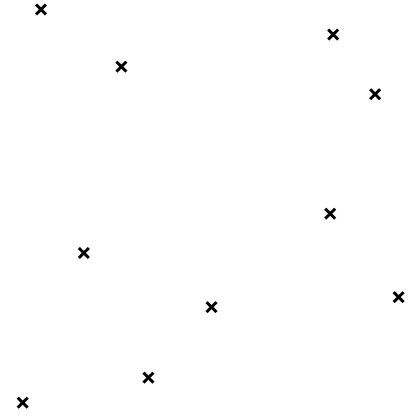
\includegraphics[width=0.35\textwidth]{img/body.png}}{\caption{Soubor bodů}}{\label{fig:soubor_bodu}}
\ffigbox{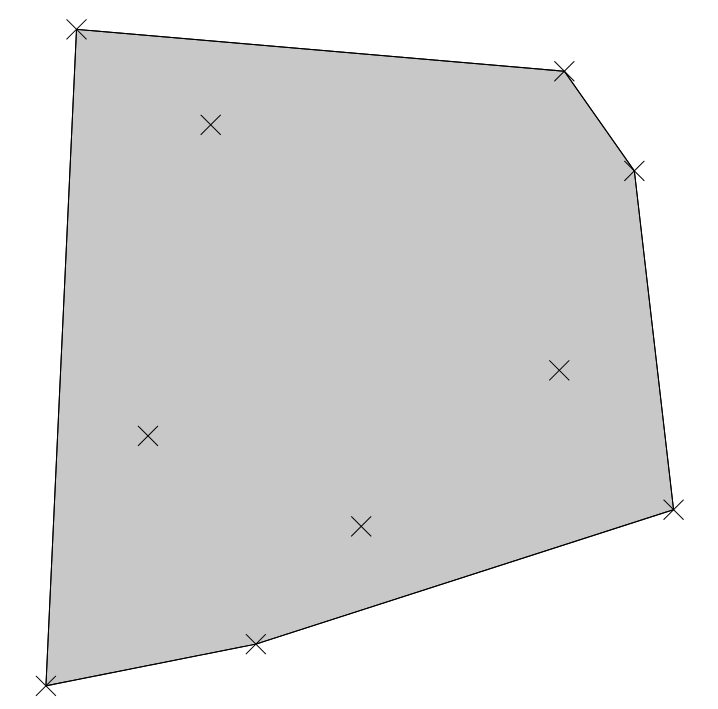
\includegraphics[width=0.35\textwidth]{img/domain.png}}{\caption{Konvexní obal nad doménou $\Omega$ }}{\label{fig:domena}}
\end{floatrow}
\end{figure}

\newpage
\subsection{Validní a regulérní triangulace}

%%% ML: neni triangulace proces, postup?
%%% AL: opraveno
Triangulace je proces vytváření trojúhelníkové
sítě mezi body v prostoru. Ne všechny trojúhelníkové sítě jsou pro nás ale zajímavé. Proto se tato práce bude zabývat triangulační
sítí se specifickými vlastnostmi.

\begin{itemize}
\item Žádný z trojúhelníků $t_{ijk}$ není zdegenerovaný, tzn. že vrcholy $i, j, k$ neleží na přímce.
\end{itemize}
\begin{figure}[h!]
\centering
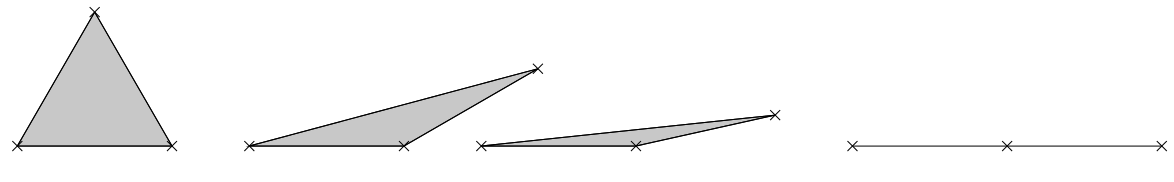
\includegraphics[width=0.9\textwidth]{img/podm_1.png}
\caption{Degenerace trojúhelníku}
\label{fig:podm_1}
\end{figure}
\begin{itemize}
\item Žádná dvojice trojúhelníků se nepřekrývá, tzn. $Int(t_{ijk}) \cap Int(t_{lmn}) = \emptyset$.
\end{itemize}
\begin{figure}[h!]
\centering
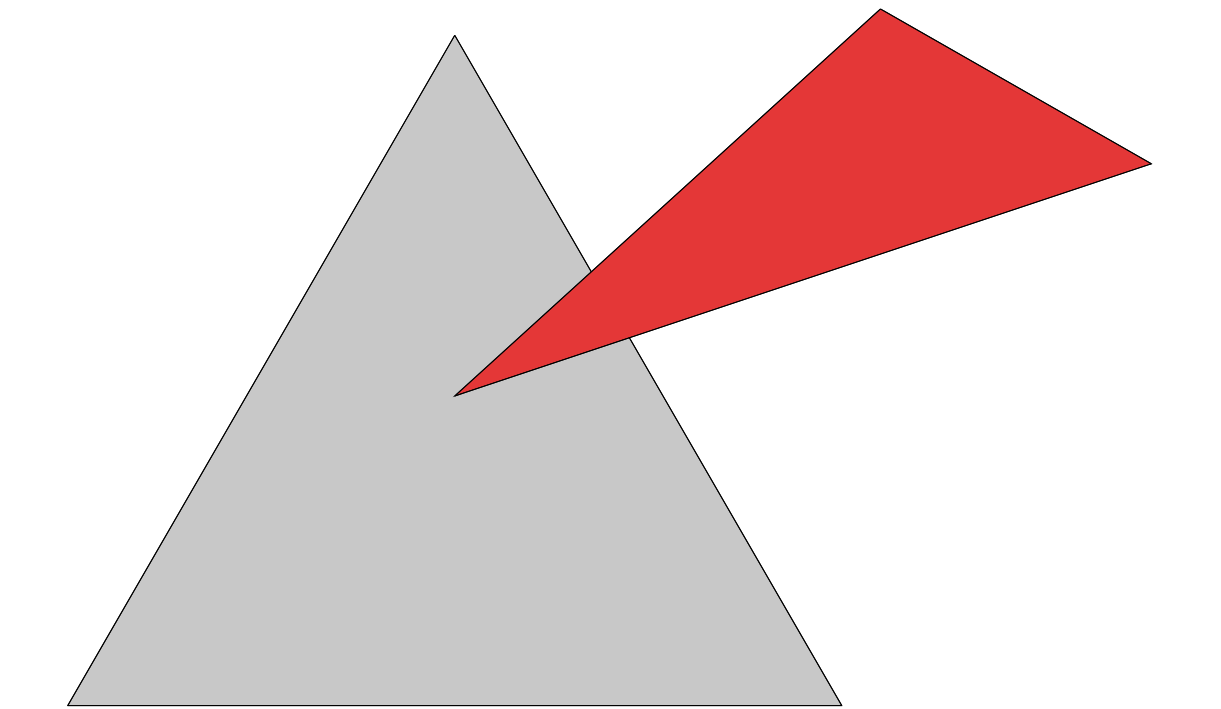
\includegraphics[width=0.25\textwidth]{img/podm_2.png}
\caption{Překrývající se trojúhelníky}
\label{fig:podm_2}
\end{figure}
\begin{itemize}
\item Hranice dvou trojúhelníků se setkávají pouze na jejich hranách
  nebo v jejich vrcholech.

\item Sjednocení všech trojúhelníků v celé triangulační síti se rovná
  celé doméně $\Omega$, nad kterou triangulaci provádíme.

\item Doména $\Omega$ musí být spojitá.

\item Triangulační síť nesmí obsahovat díry.

\item Jestliže vrchol $v_i$ leží na hranici konvexního obalu, pak musí
  existovat právě dvě hraniční hrany, které mají vrchol $v_i$ jako
  společný vrchol. To mimo jiné znamená, že počet hraničních vrcholů
  je roven počtu hraničních hran.
\end{itemize}
\bigskip

Pokud jsou naplněny první čtyři podmínky, může se triangulace nazvat
\emph{validní}. V případě, že naplníme všech sedm podmínek, dá se
mluvit o \emph{regulérní} triangulaci.

\begin{figure}[h!]
\centering
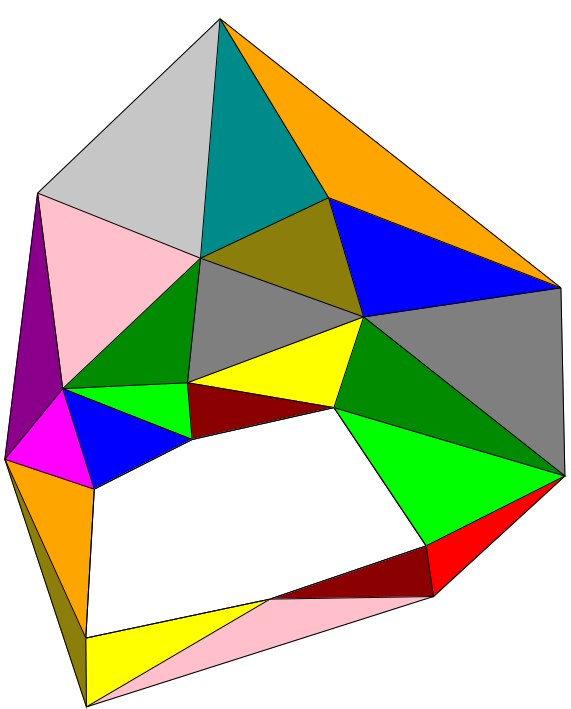
\includegraphics[width=0.35\textwidth]{img/podm_domena.png}
\caption{Nespojitá doména, triangulace obsahující díry}
\label{fig:podm_domena}
\end{figure}

\begin{figure}[h!]
\centering
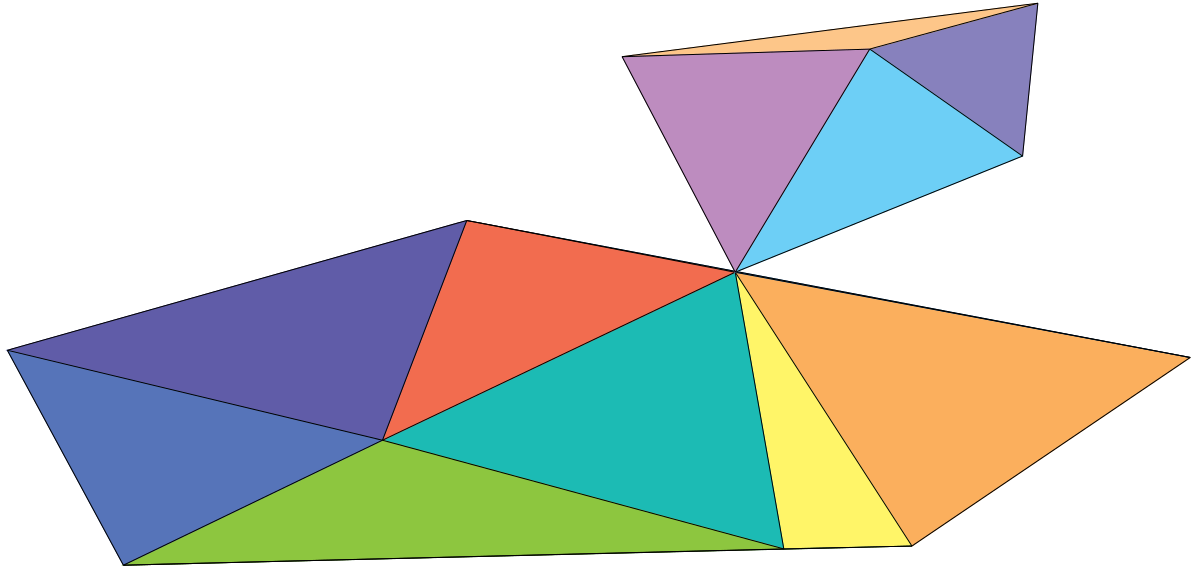
\includegraphics[width=0.9\textwidth]{img/vnr.png}
\caption{Triangulace validní, ale neregulérní}
\label{fig:trian_valid_not_reg}
\end{figure}

%%% ML: osobne bych psal na techto mistech Obrazek s malym pismenem,
%%% predpokladam, ze vychazis z Figure, v cestine jsou jina pravidla,
%%% to je ale detail
%%% AL: prepsano na obrazek
V případě triangulace na obrázku \ref{fig:trian_valid_not_reg} se
jedná o triangulaci validní, neboť splňuje všechny z prvních čtyř
%%% ML: odkazujes na podminky cislem, potom bych pro jejich vycet
%%% pouzil enumerate a ne itemize
%%% AL: puvodne tam byl enumerate, ale mel jsem problem s vkladanim obrazku do seznamu. Prepsal jsem odkazy na cisla
podmínek. Nicméně nesplňuje poslední podmínku, neboť existují více jak
právě dvě hraniční hrany, které vstupují do jednoho vrcholu na
konvexním obalu, a triangulaci tedy nelze nazvat i regulérní.

\begin{figure}[h!]
\centering
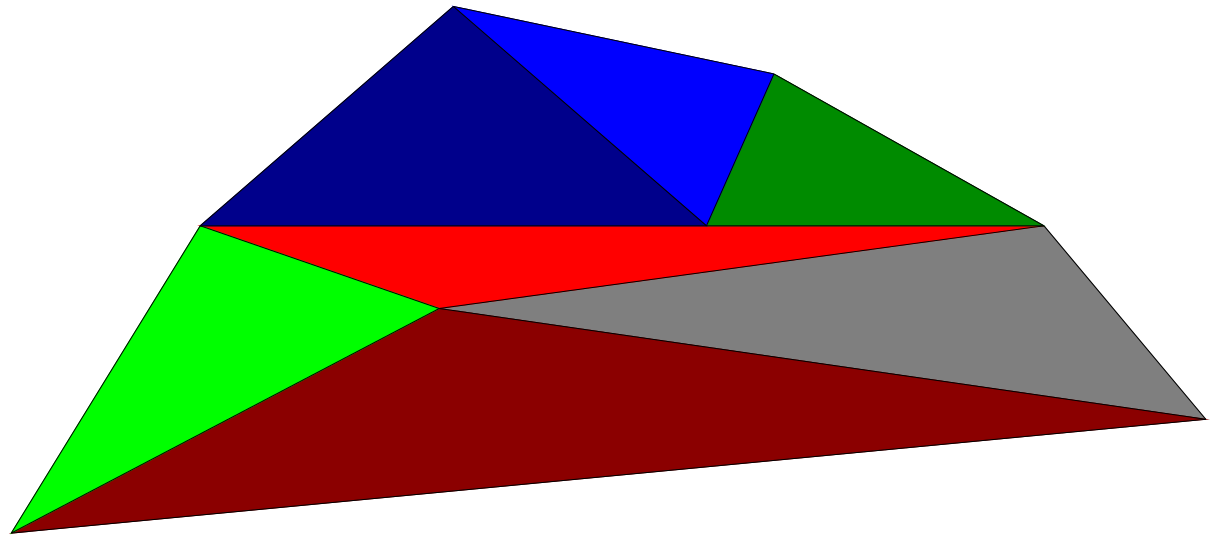
\includegraphics[width=0.9\textwidth]{img/nv.png}
\caption{Triangulace nevalidní}
\label{fig:train_not_valid}
\end{figure}

\newpage

Triangulace na obrázku \ref{fig:train_not_valid} není validní, protože
nesplňuje podmínku č. 3. Tím pádem se nejedná ani o triangulaci
regulérní.

\begin{figure}[h!]
\centering
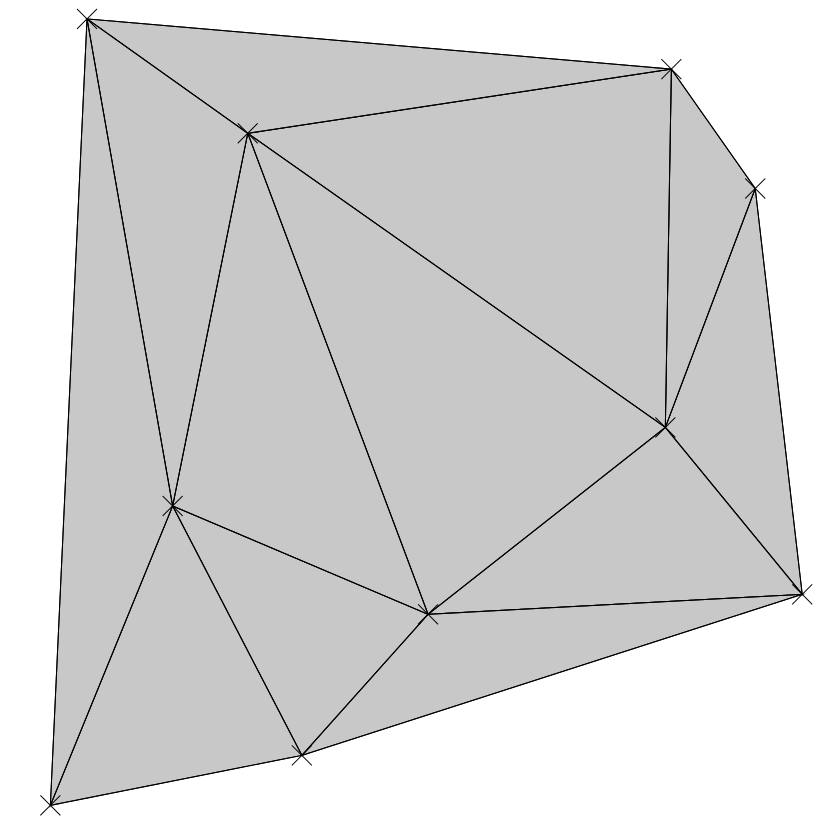
\includegraphics[width=0.9\textwidth]{img/triangulation.png}
\caption{Regulérní triangulace}
\label{fig:triangulace}
\end{figure}

Na obrázku \ref{fig:triangulace} už můžeme vidět validní a regulérní
triangulaci. Jedná se též o triangulaci \emph{optimální}, což je
termín, kterým se budeme zabývat v kapitole \ref{subsec:Optim_trian}.

\newpage
\subsection{Optimální triangulace}
\label{subsec:Optim_trian}

Nad doménou $\Omega$ neexistuje pouze jediná trojúhelníková síť, v
závislosti na počtu bodů v množině a jejich konfiguraci existuje
poměrně velké množství možností, jak může trojúhelníková síť
vypadat. Ne všechny sítě jsou však vhodné k dalšímu zpracovávání, a
právě proto je snaha najít \emph{optimální} triangulaci.

Při řešení otázky, jak vypadá optimální triangulace, je zásadní
zamyslet se nad tvarem trojúhelníků. V ideálním případě by byly
všechny trojúhelníky rovnostranné, leč tento případ se v případě
náhodně roztroušených dat nevyskytuje.

Při tvorbě optimální triangulace se tedy problém řeší z opačného
konce. Zásadní snahou při tvorbě sítě by mělo být vyhýbání se
podlouhlým, štíhlým nebo téměř degenerovaným trojúhelníkům, tedy
trojúhelníkům s příliš ostrými nebo s příliš tupými úhly.

\paragraph{Kruhová podmínka}
~\newline
Definice: Nechť hrana $\overline{p_ip_j}$ inciduje s trojúhelníkem
$t_1$ tvořeným vrcholy $p_i,p_j,p_k$ a trojúhelníkem $t_2$ tvořeným
vrcholy $p_i,p_j,p_l$ a kružnice $k$ procházející body
$p_i,p_j,p_k$. Hrana $\overline{p_ip_j}$ je nelegální tehdy a právě
jen tehdy, jestliže bod $p_l$ leží uvnitř $k$.

Pokud tedy bod $p_l$ leží uvnitř kružnice $k$, je hrana
$\overline{p_ip_j}$ a tedy diagonála čtyřúhelníku nelegální, stejně
tak jako oba trojúhelníky $t_1$ a $t_2$. K jejich legalizaci je
provést tzv. \emph{Edge swaping}.

\paragraph{MaxMin a MinMax úhlová podmínka}\cite{TB1}

Pokud nad množinou bodů P provedeme všechny možné triangulace, můžeme
nejoptimálnější triangulaci určit pomocí MaxMin popř. MinMax
podmínky. V případě MaxMin podmínky je pro každou možnou triangulaci
nalezen největší minimální vnitřní úhel trojúhelníku a ten je porovnán
s největším minimálním úhlem ostatních triangulací, což vede k
eliminaci trojúhelníků s velmi tupými úhly. U MinMax podmínky se
postupuje obdobně, pouze se porovnávají nejmenší maximální vnitřní
úhly trojúhelníků a eliminují se tak trojúhelníky s velmi ostrými
úhly.

\newpage
{\bf MinMax podmínka} Eliminace trojúhelníků s příliš tupými
úhly. Triangulace $\Delta(P)$ je vzhledem k tomuto kritériu na rozdíl
od triangulace $\Delta^{'}(P)$ optimální, je–li největší úhel $\alpha$
generovaný triangulací $\Delta(P)$ je menší než největší úhel
$\alpha^{'}$ generovaný triangulací $\Delta^{'}(P)$.
\begin{center}
$\alpha_{max} = max(\alpha_i(\Delta))$

$\alpha^{'}_{max} = max(\alpha_i^{'}(\Delta))$

$\alpha_{max} < \alpha^{'}_{max}$
\end{center}

\bigskip

{\bf MaxMin podmínka} Eliminace trojúhelníků s příliš ostrými
úhly. Triangulace $\Delta(P)$ je vzhledem k tomuto kritériu na rozdíl
od triangulace $\Delta^{'}(P)$ optimální, je–li nejmenší úhel $\alpha$
generovaný triangulací $\Delta(P)$ je větší než nejmenší úhel
$\alpha^{'}$ generovaný triangulací $\Delta^{'}(P)$.
\begin{center}
$\alpha_{min} = min(\alpha_i(\Delta))$

$\alpha^{'}_{min} = min(\alpha_i^{'}(\Delta))$

$\alpha_{min} > \alpha^{'}_{min}$
\end{center}

\paragraph{Neutrální případ pro MaxMin podmínku}

Problém nastává ve chvíli, kdy některé body, mezi kterými chceme
triangulaci provést, leží na kružnici nebo se tomu limitně blíží. V
takových chvílí nastává takzvaný neutrální případ pro MaxMin
podmínku. V některých případech to může vést k nejednoznačnému určení,
která z~triangulací je optimální a musíme si pomoci hodnocením na
základě nejen MaxMin ale i MinMax podmínky.

\begin{figure}[h!]
\centering
\begin{floatrow}
\ffigbox{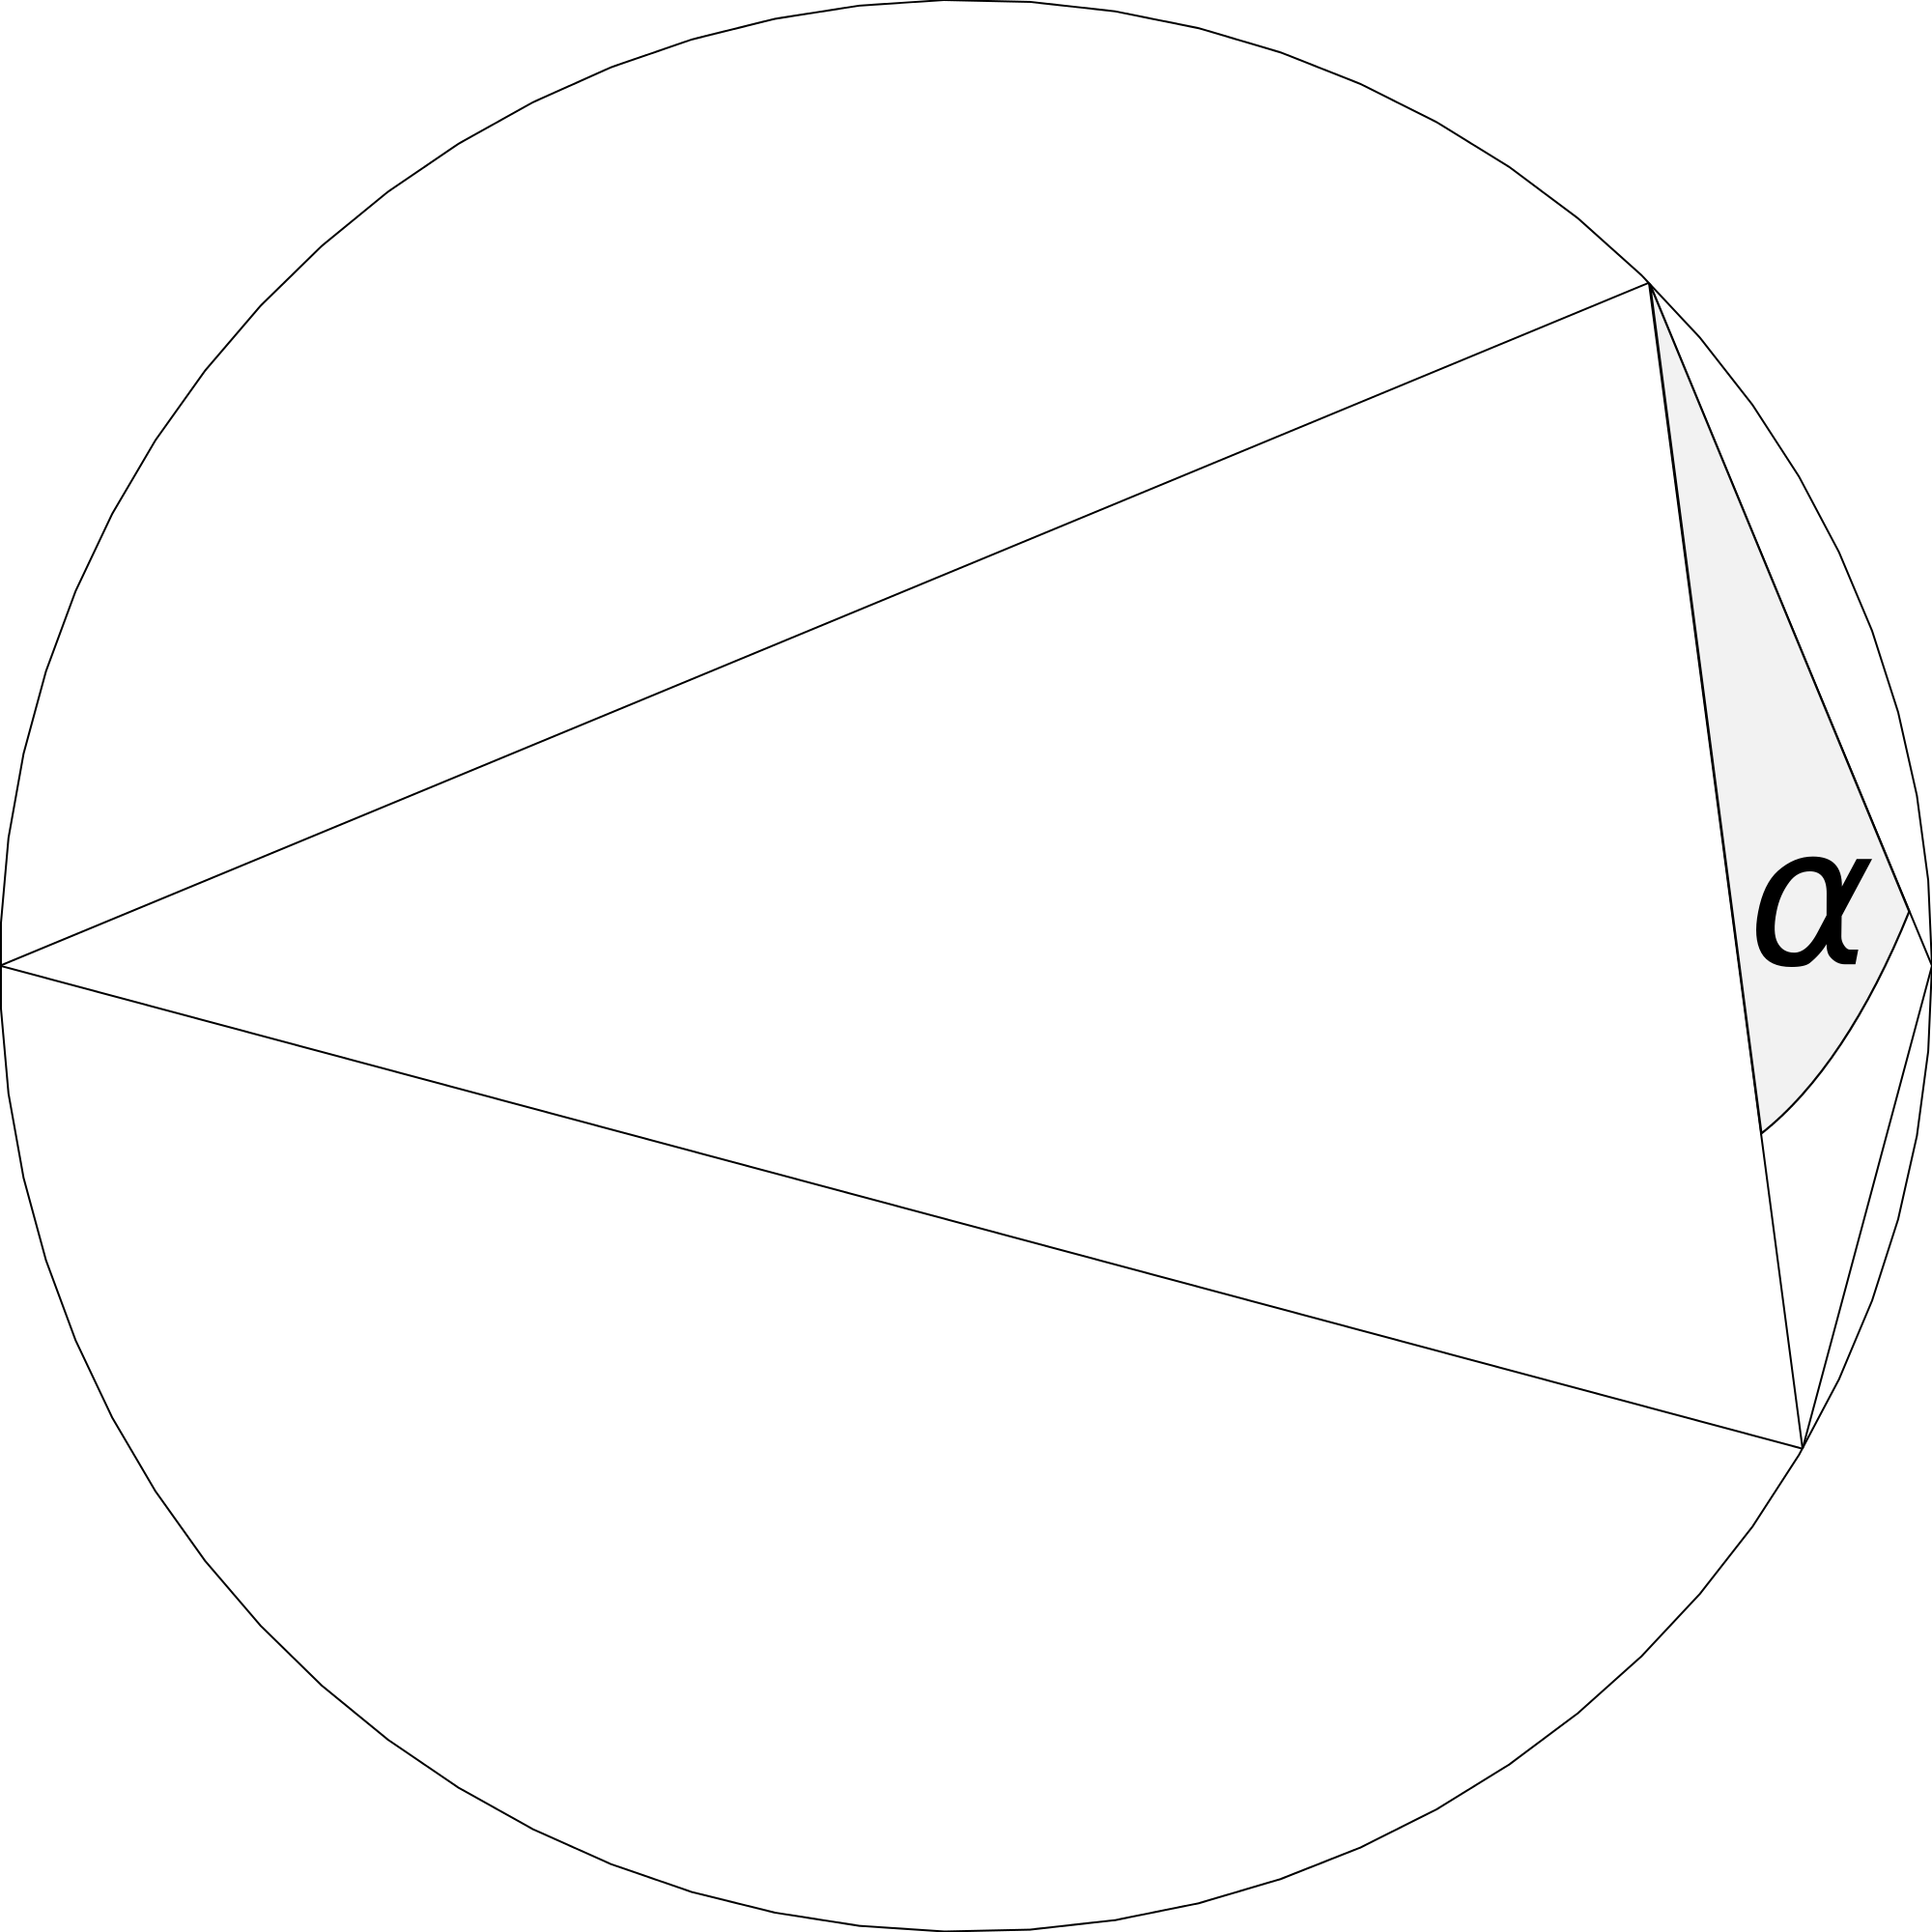
\includegraphics[width=0.48\textwidth]{img/minmax2_pokus.png}}{\caption{Případ 1}\label{fig:neutral_case_1}}
\ffigbox{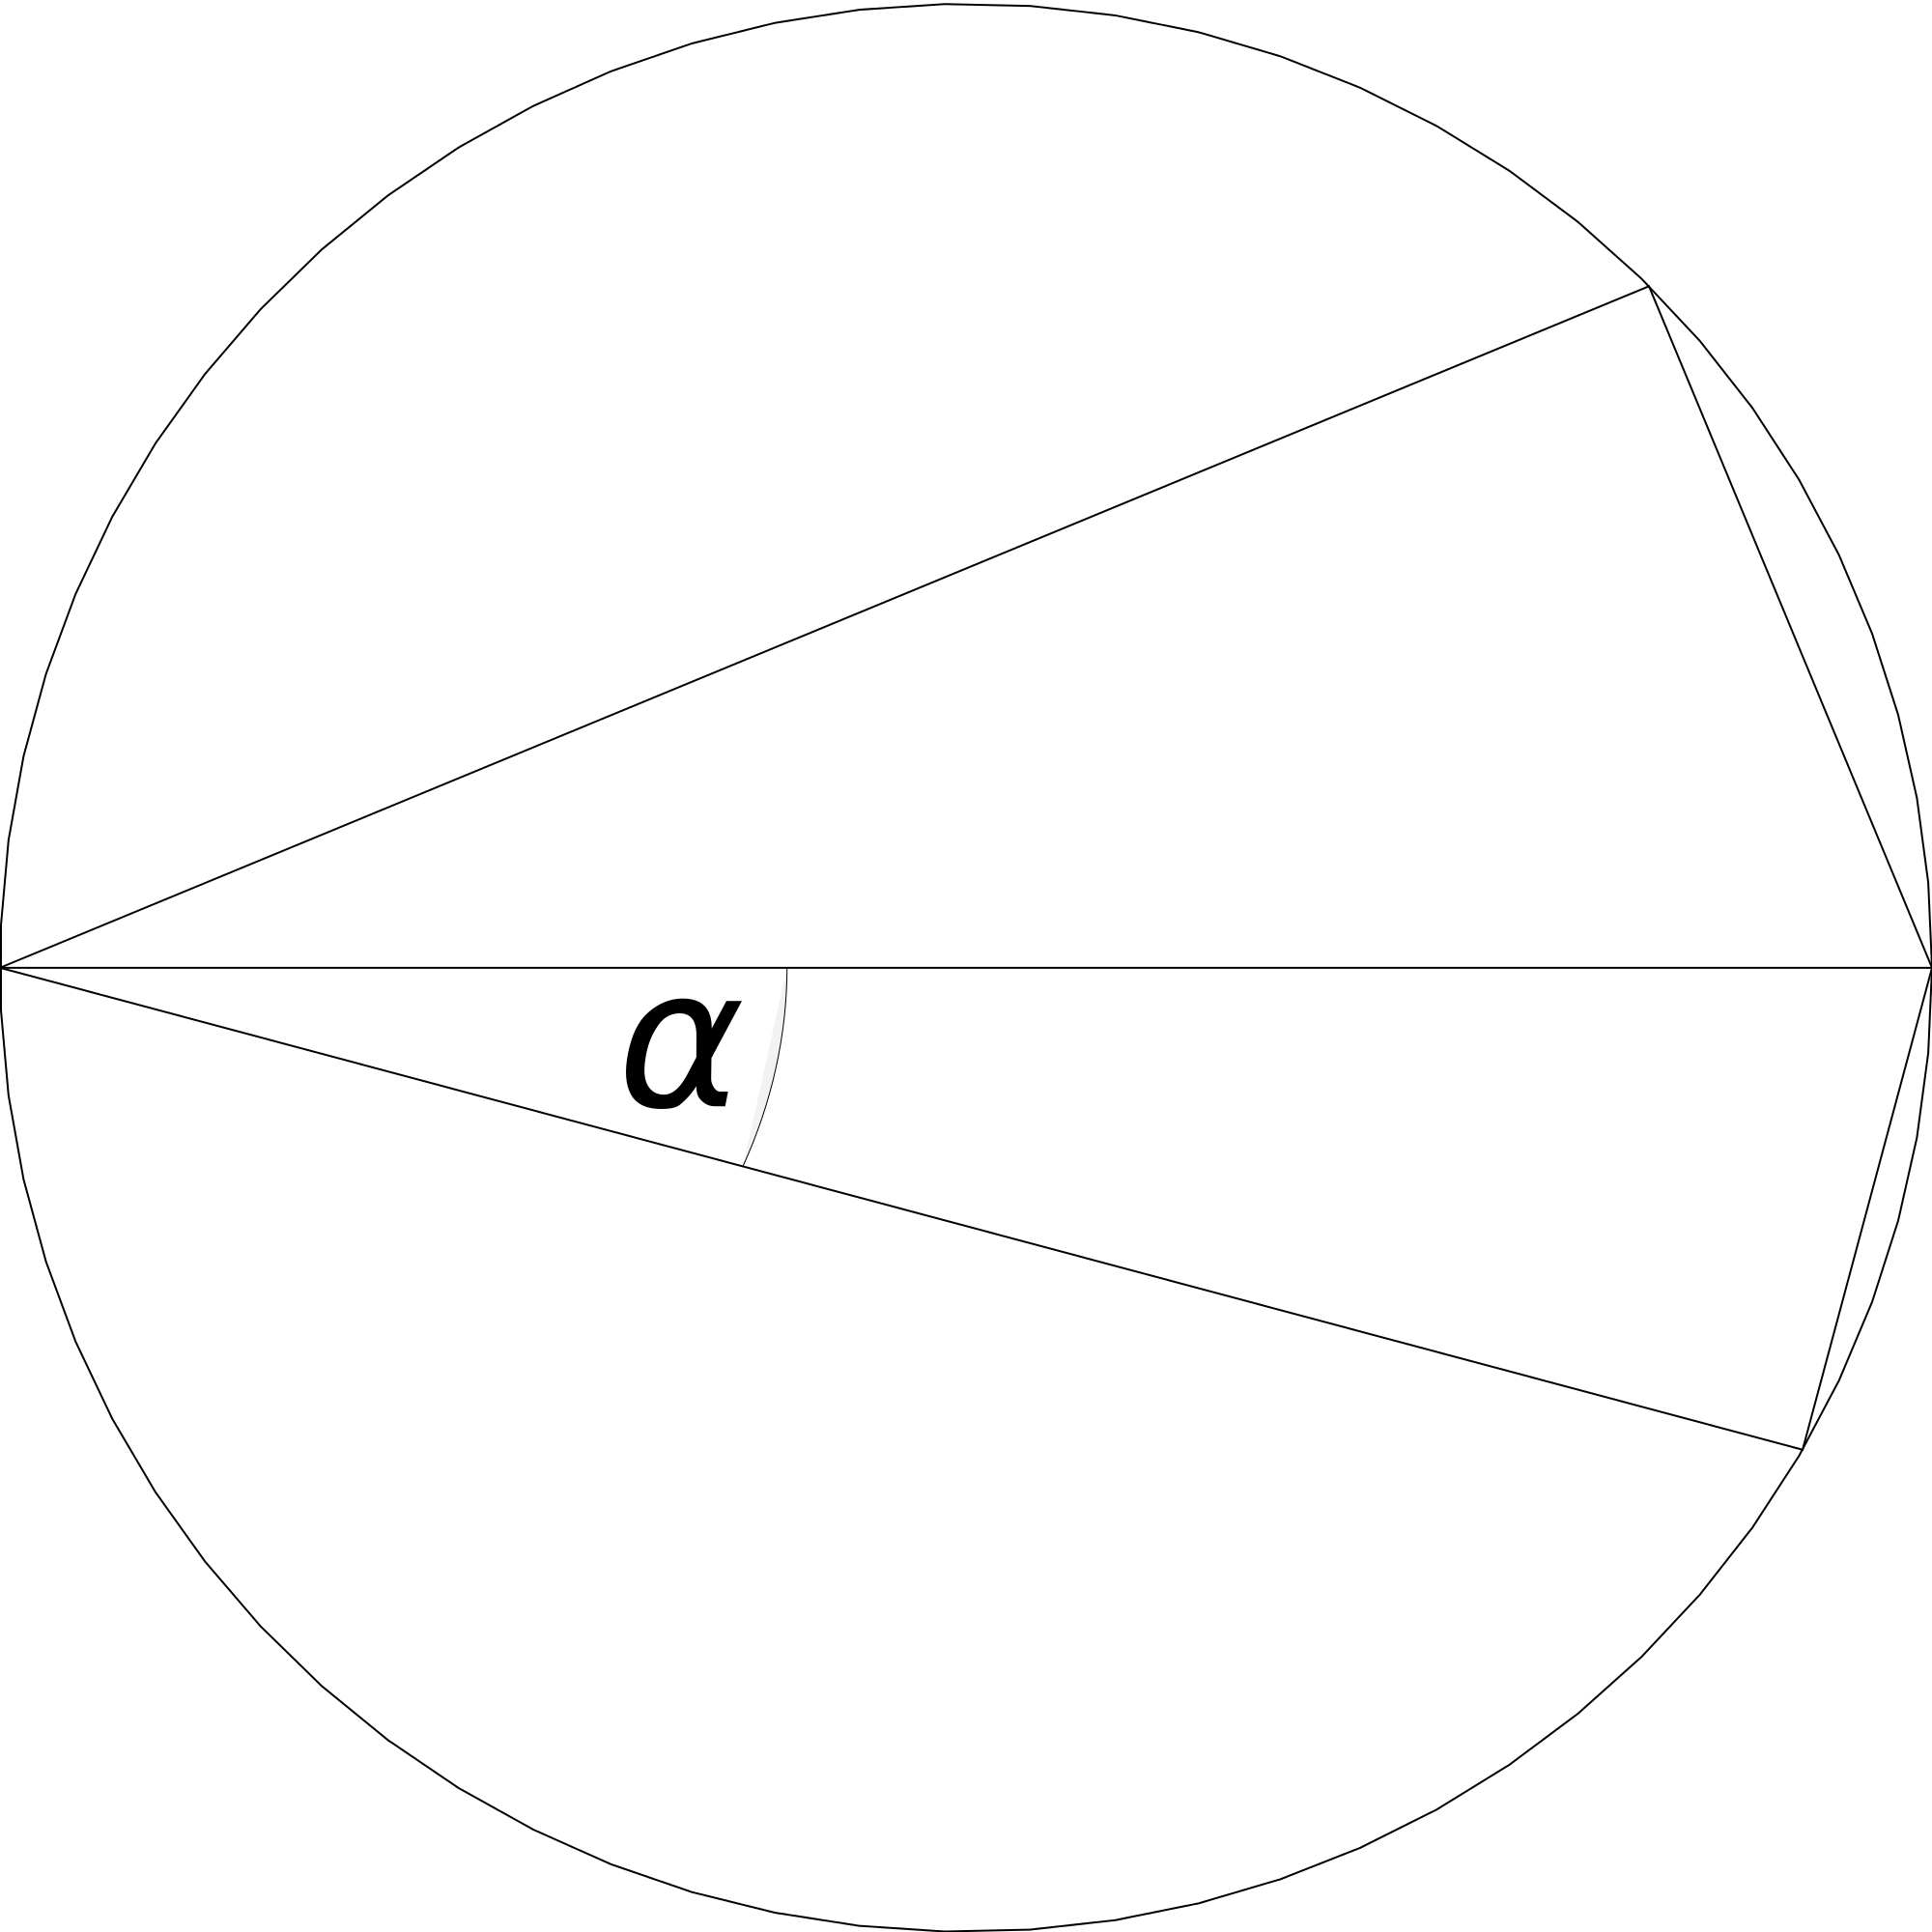
\includegraphics[width=0.48\textwidth]{img/minmax1_pokus.png}}{\caption{Případ 2}\label{fig:neutral_case_2}}
\end{floatrow}
\end{figure}


Nejčastěji tento jev nastává u čtyřúhelníku, jehož všechny vrcholy
leží na kružnici. Jak je vidět na obrázcích \ref{fig:neutral_case_1} a
\ref{fig:neutral_case_2}, maximální minimální úhel triangulace je
v~obou případech úhel $\alpha$, což je obvodový úhel nejkratší strany
čtyřúhelníku. V~tomto případě se jedná o neutrální případ pro MaxMin
podmínku. Pokud by tedy triangulace byla hodnocena pouze na základě
MaxMin podmínky, mohly by být obě triangulace prohlášeny za
optimální. Už od pohledu je ale zřejmé, že lepší tvar trojúhelníků
poskytujeme triangulace na obrázku \ref{fig:neutral_case_1}. Pokud je
ale triangulace hodnocena i s ohledem na MinMax podmínknu, je
prokázáno, že triangulace na obrázku \ref{fig:neutral_case_2} je
optimální.


\paragraph{Edge swaping, legalizace}

Na obrázcích \ref{fig:neutral_case_1} a \ref{fig:neutral_case_2} jsme
si ukázali případ neutrálního případu pro MinMax podmínku. Proces, při
kterém jsme zaměnili diagonálu čtyřúhelníku tak, aby byli oba
trojúhelníky lokálně optimální, se nazývá \emph{Edge swaping.} Pokud
budeme tento proces aplikovat pro celou triangulaci dojde k takzvané
\emph{legalizaci} triangulace.

\paragraph{Delaunayova triangulace}

Triangulace, která je optimální dle kruhové nebo MaxMin úhlové
podmínky a která je definována nad konvexním obalem množiny bodů, se
nazývá \emph{Delaunayova triangulace}\footnote{Delaunayova triangulace
  je pojmenována podle ruského matematika Borise Nikolaeviche
  Delaunayho\cite{Delaunay}, který ji definoval v roce 1934.}.

\newpage
\subsection{Voronoiův diagram}

Voronoiův diagram souvisí s Delaunayovou triangulací. Představme si
opět množinu bodů $P = \{p_1,...p_N\} $ v rovině $E^2$ a nechť je
$d(p_i,p_j) $ Eukleidovská vzdálenost mezi body $p_i$ a $p_j$. Rovinu
poté rozdělíme na oblasti $V(p_i,...,p_N)$, kde každému bodu $p_i$ z
množiny $P$ přiřadíme takovou oblast, která splňuje následující
podmínku:

$V(p_i) = \{ x: d(x, p_i) < d(x, p_j), j = 1,...,N\}$.

Pro každou takovouto oblast přiřazenou bodu $p_i$ platí, že
všechny body uvnitř této oblasti jsou k bodu $p_i$ blíž než ke
kterémukoliv jinému bodu z množiny $P$. Toto rozdělení roviny se
nazývá \emph{Voronoiův diagram (VD)} množiny bodů a každá uzavřená
buňka se nazývá \emph{Voronoiova buňka.}

\bigskip
Voronoiův diagram má následující vlastnosti: 
\begin{itemize}
\item Voronoiův diagram pro množinu bodů je pouze jeden.
\item Všechny oblasti jsou konvexní.
\item Oblast $V(p_i)$ obsahuje jediný bod $p_i \in P$.
\item Oblasti na okraji jsou neohraničené.
\item Počet hran a uzlů je přímo úměrný počtu bodů v množině P.
\item Pokud žádné 4 body neleží na kružnici, uzly mají stupeň 3.
\item Uzel leží ve středu kružnice určené 3 body z P, které leží v přilehlých oblastech a neleží na přímce.
\end{itemize}

Nechť $H(p_i,P_j)$ je polorovina obsahující všechny body v rovině,
jejichž vzdálenost od bodu $p_i$ je menší než od bodu $p_j$. Potom
Voronoiova oblast $V(p_i)$ je průnikem $N-1$ polorovin,
$V(p_i)= \bigcap\limits_{\substack{j=1,...,N \\ i\not=j}}H(p_i,p_j)$,
kde každá oblast má maximálně $N-1$ stran.

\newpage
\begin{figure}[h!]
\centering
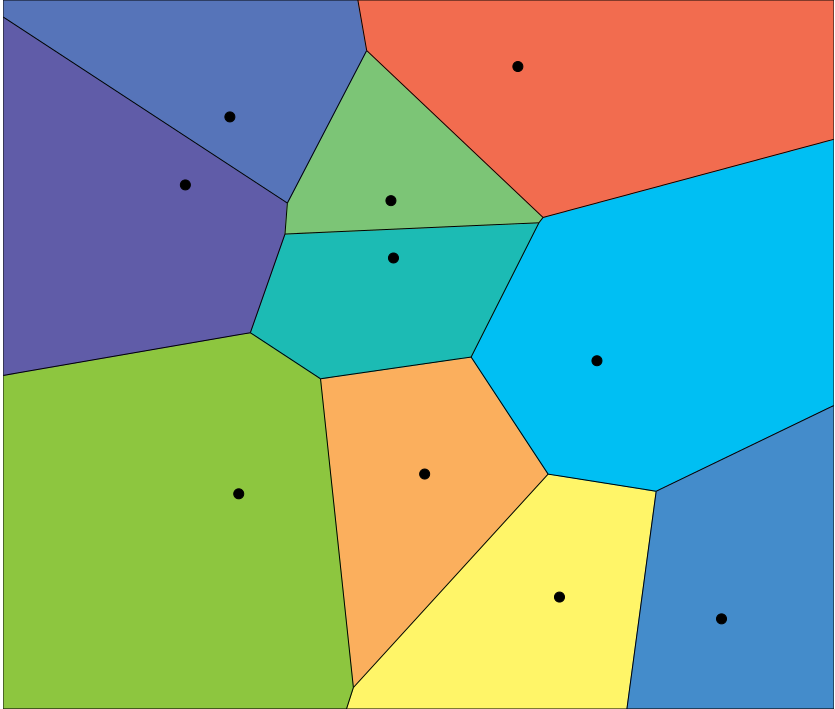
\includegraphics[width=0.7\textwidth]{img/vor_pol.png}
%%% ML: Opravdu polygony, nepouziva se termin bunka?
%%% AL: Resil jsem s TB, existuje termin polygon, ale v tomhle pripade to maji byt bunky, opraveno
\caption{Voronoivy buňky}
\label{fig:vor_pol}
\end{figure}

Z obrázku \ref{fig:vor_pol} je vidět, že oblasti přiřazené pro body na
okraji konvexního obalu nejsou zcela ohraničené a uzavřené. Jednotlivé
hranice oblastí nazýváme \emph{Voronoiovy polygony}, které jsou
složeny z takzvaných \emph{Voronoiových hran a bodů}. O dvou bodech
$p_j$ a $p_k$ můžeme tvrdit, že jsou \emph{Voronoiovi sousedé}, pokud
oblasti, kterým náleží, sdílí společnou \emph{Voronoiovu hranu}.

Občas se můžeme setkat i s označením \emph{Thiessenovy polygony} podle
klimatologa Thiessena, který Voronoiovi diagramy používal k
interpolaci klimatických dat z náhodně distribuovaných
meteorologických stanic.

\newpage
\subsection{Voronoiovy diagramy a Delaunayova triangulace}
\label{sub:VDaDT}

%%% ML: poznamka pod carou, co je planarni graf (nebo je to vysvetleno jinde?)
%%% AL: pridan footnote, staci takhle?
DT je planární graf\footnote{Planární graf je takový graf, který lze v rovině nakreslit bez křížení hran.}, který je duální k VD. Jedna konstrukce tedy může
být odvozena od druhé a naopak.  Pokud pro množinu bodů v rovině
provedeme rozdělení do Voronoiových diagramů a následně spojíme
úsečkami všechny Voronoiovi sousedy získáme Delaunayovu triangulaci.

\begin{figure}[h!]
\centering
\begin{floatrow}
\ffigbox{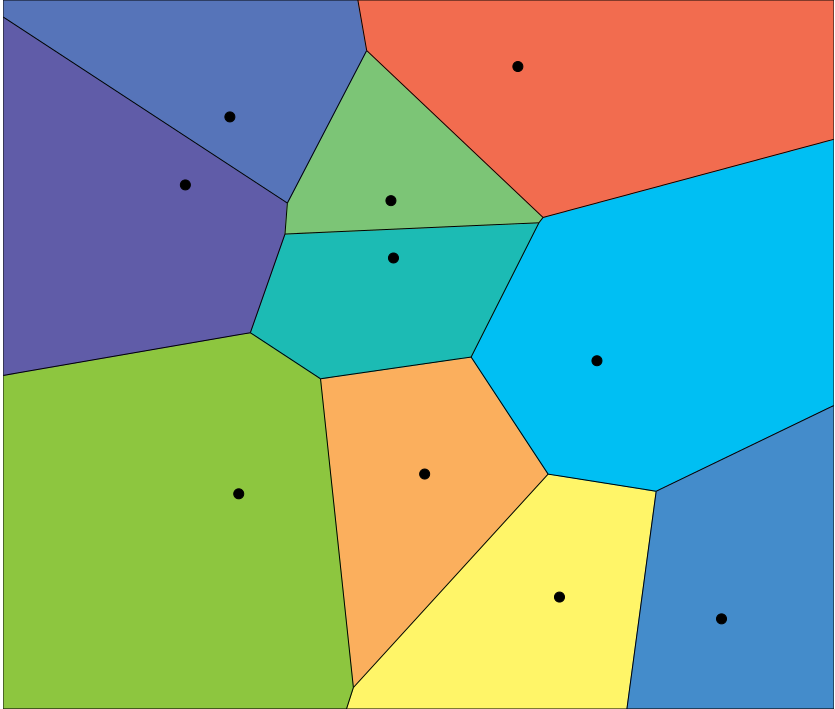
\includegraphics[width=0.45\textwidth]{img/vd_vor.png}}
{\caption{Voronoiův diagram souboru bodů}\label{fig:vd_vor}}
\ffigbox{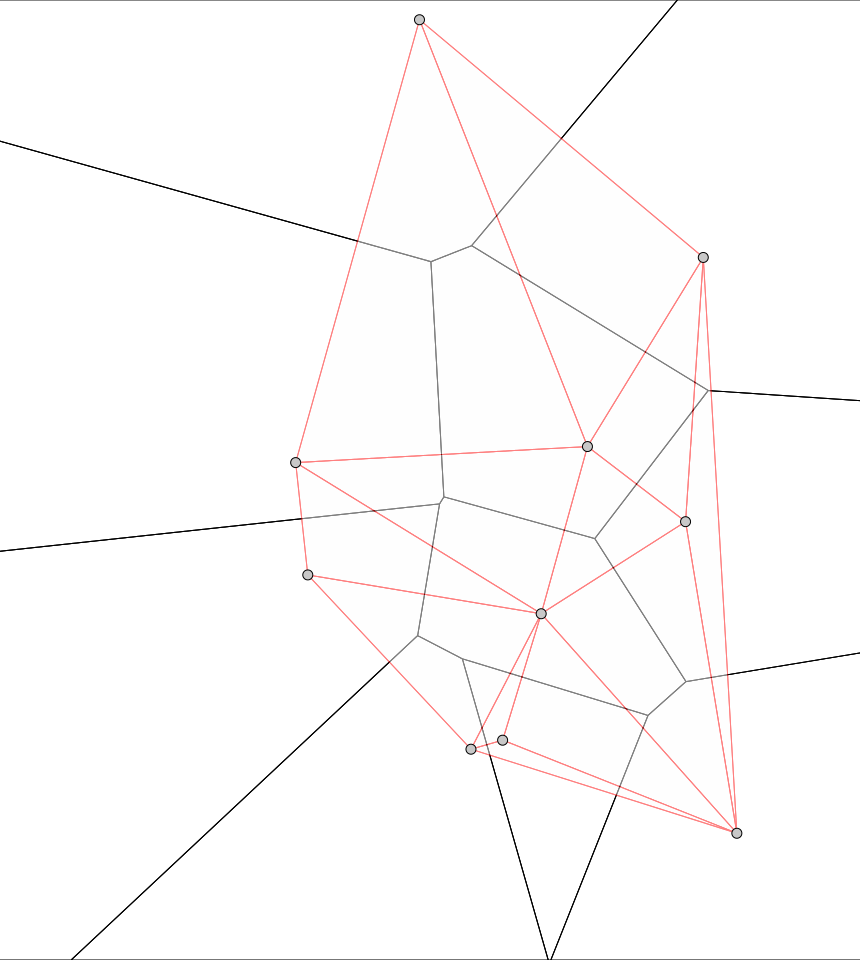
\includegraphics[width=0.45\textwidth]{img/vd_del.png}}
{\caption{Voronoiův diagram a Delaunayova trinagulace}\label{fig:vd_del}}
\end{floatrow}
\end{figure}

Na obrázku \ref{fig:vd_vor} můžeme vidět Voronoiův diagram pro množinu
bodů. Pokud každou dvojici Voronoiových sousedů spojíme spojnicí, jak
je vidět na obrázku \ref{fig:vd_del}, získáme několik trojúhelníků,
které se nepřekrývají a tvoří trojúhelníkovou síť. Spojnice mezi body,
které jsou přiřazeny k neuzavřeným oblastím, tvoří konvexní obal. Pro
trojúhelníkovou síť uvnitř tohoto konvexního obalu se jedná o
Delaunayovu triangulaci.

Trojúhelníky této sítě se nazývají \emph{Delaunayovi trojúhelníky},
které jsou tvořeny spojnicemi tzv. \emph{Delaunayvými hranami}. Dále
je také zřejmé, že Voronoiovy hrany leží na ose Delaunayových hran.


\newpage
\section{Algoritmy pro tvorbu DT}
\label{sec:algoritmy}
Triangulační algoritmy jsou poměrně dobře matematicky prozkoumaná
oblast, ke kterým je k dispozici široký teoretický základ. Při hledání
vhodného algoritmu je třeba zohlednit následující požadavky:
\begin{itemize}
\item Jednoduchost algoritmu a jeho snadná implementace.
\item Dostatečná rychlost i pro velké množiny bodů (n>1E6), ideálně aby se výpočetní čas blížil $O(n . log(n))$.
\item Malá citlivost a vysoká stabilita pro případy nejednoznačné triangulace (body na kružnici).
\item Převod do vyšších dimenzí.
\item Možnost paralelizace algoritmu.
\end{itemize}
Vhodný algoritmus je vhodné vybírat na základě datových struktur a
konkrétním případu. Ne vždy lze dokonale splnit všechny požadavky,
např. jednoduché implementace mají delší výpočetní čas. Naopak
algoritmy s kratším výpočetním časem jsou dost náročné na
implementaci.

\newpage
\subsection{Lokální optimalizace}
\emph{Lokální optimalizace (LO)} je proces přetvoření libovolné
triangulace na DT. Proces je prováděn pomocí prohazování nelegálních
hran v dvojicích trojúhelníků tvořících konvexní čtyřúhelník na
%%% ML: v cestine se na techto mistech pise male pismeno, ale je
%%% mozne, ze se to podle novych pravidel pravopisu zmenilo a je mozne
%%% i psat velka pismena v tomto kontextu (je to na vice mistech v
%%% textu)
%%% AL: Nad tim jsem uvazoval. Nakonec tedy pisu s malym k. MaxMin a MinMax jsem nechal, prijde mi to prehlednejsi
základě kruhové nebo MaxMin podmínky.

Pro množinu bodu $P$ nechť $e_i$ je vnitřní hrana triangulace a $Q$ je
čtyřúhelník tvořený dvěma trojúhelníky se společnou hranou
$e_i$. Možnost, že čtyřúhelník je nekonvexní nebo že všechny jeho body leží
na kružnici, nebude nyní brán v úvahu. Poté je za použití MaxMin nebo
kruhové podmínky rozhodnuto, zda je třeba prohodit hranu $e_i$. V
případě, že po použití Lokální optimalizace není potřeba prohodit
hranu, můžeme dvojici trojúhelníků a jejich společnou hranu prohlásit
za lokálně optimální. V případě, že budeme lokální optimalizaci
používat opakovaně pro všechny hrany v triangulaci, dokud nebudou
všechny hrany lokálně optimální, získáme optimální triangulaci.

%%% ML: Nelze pocestit titulek (?) - detail
%%% AL: Pocesteno
\begin{algorithm}
\caption{Lokální optimalizace}
\begin{algorithmic}[1]
\State Vytvoř pomocnou triangulaci $\Delta(P)$
\State legal=false
\While{ $\Delta(P)$ != legal}
	\State legal=true
	\For{$\forall e_i \in \Delta(P)$}
		\State Vezmi hranu $e_i \in \Delta(P)$
		\State Nalezni trojúhelníky $t_1,t_2$ incidující s $e_i$.
		\If {$(t_1 \cup t_2)$ je konvexní a nelegální}
			\State Legalize $(t_1,t_2)$
			\State legal=false
		\EndIf
	\EndFor
\EndWhile	
\end{algorithmic}
\end{algorithm}

\newpage
\subsection{Paprskovitý algoritmus}

Tento algoritmus je podobný tomu předchozímu, pouze využívá jiný
postup, jak nalézt počáteční triangulaci $\Delta$. Na začátku se
nalezne bod $p$ z množiny $P$ takový, který je nejbližší jejímu
středu. Poté je paprskovitě spojen se všemi zbývajícími body množiny
$P$. Tyto body se následně seřadí podle orientace a vzdálenosti od
bodu $p$ a v tomto pořadí se spojí hranami. Potom se vytvoří hrany na
hranici triangulace. Vzniklá triangulace se dále postupně po
jednotlivých hranách legalizuje stejně jako v předchozím případě.

\begin{figure}[h!]
\centering
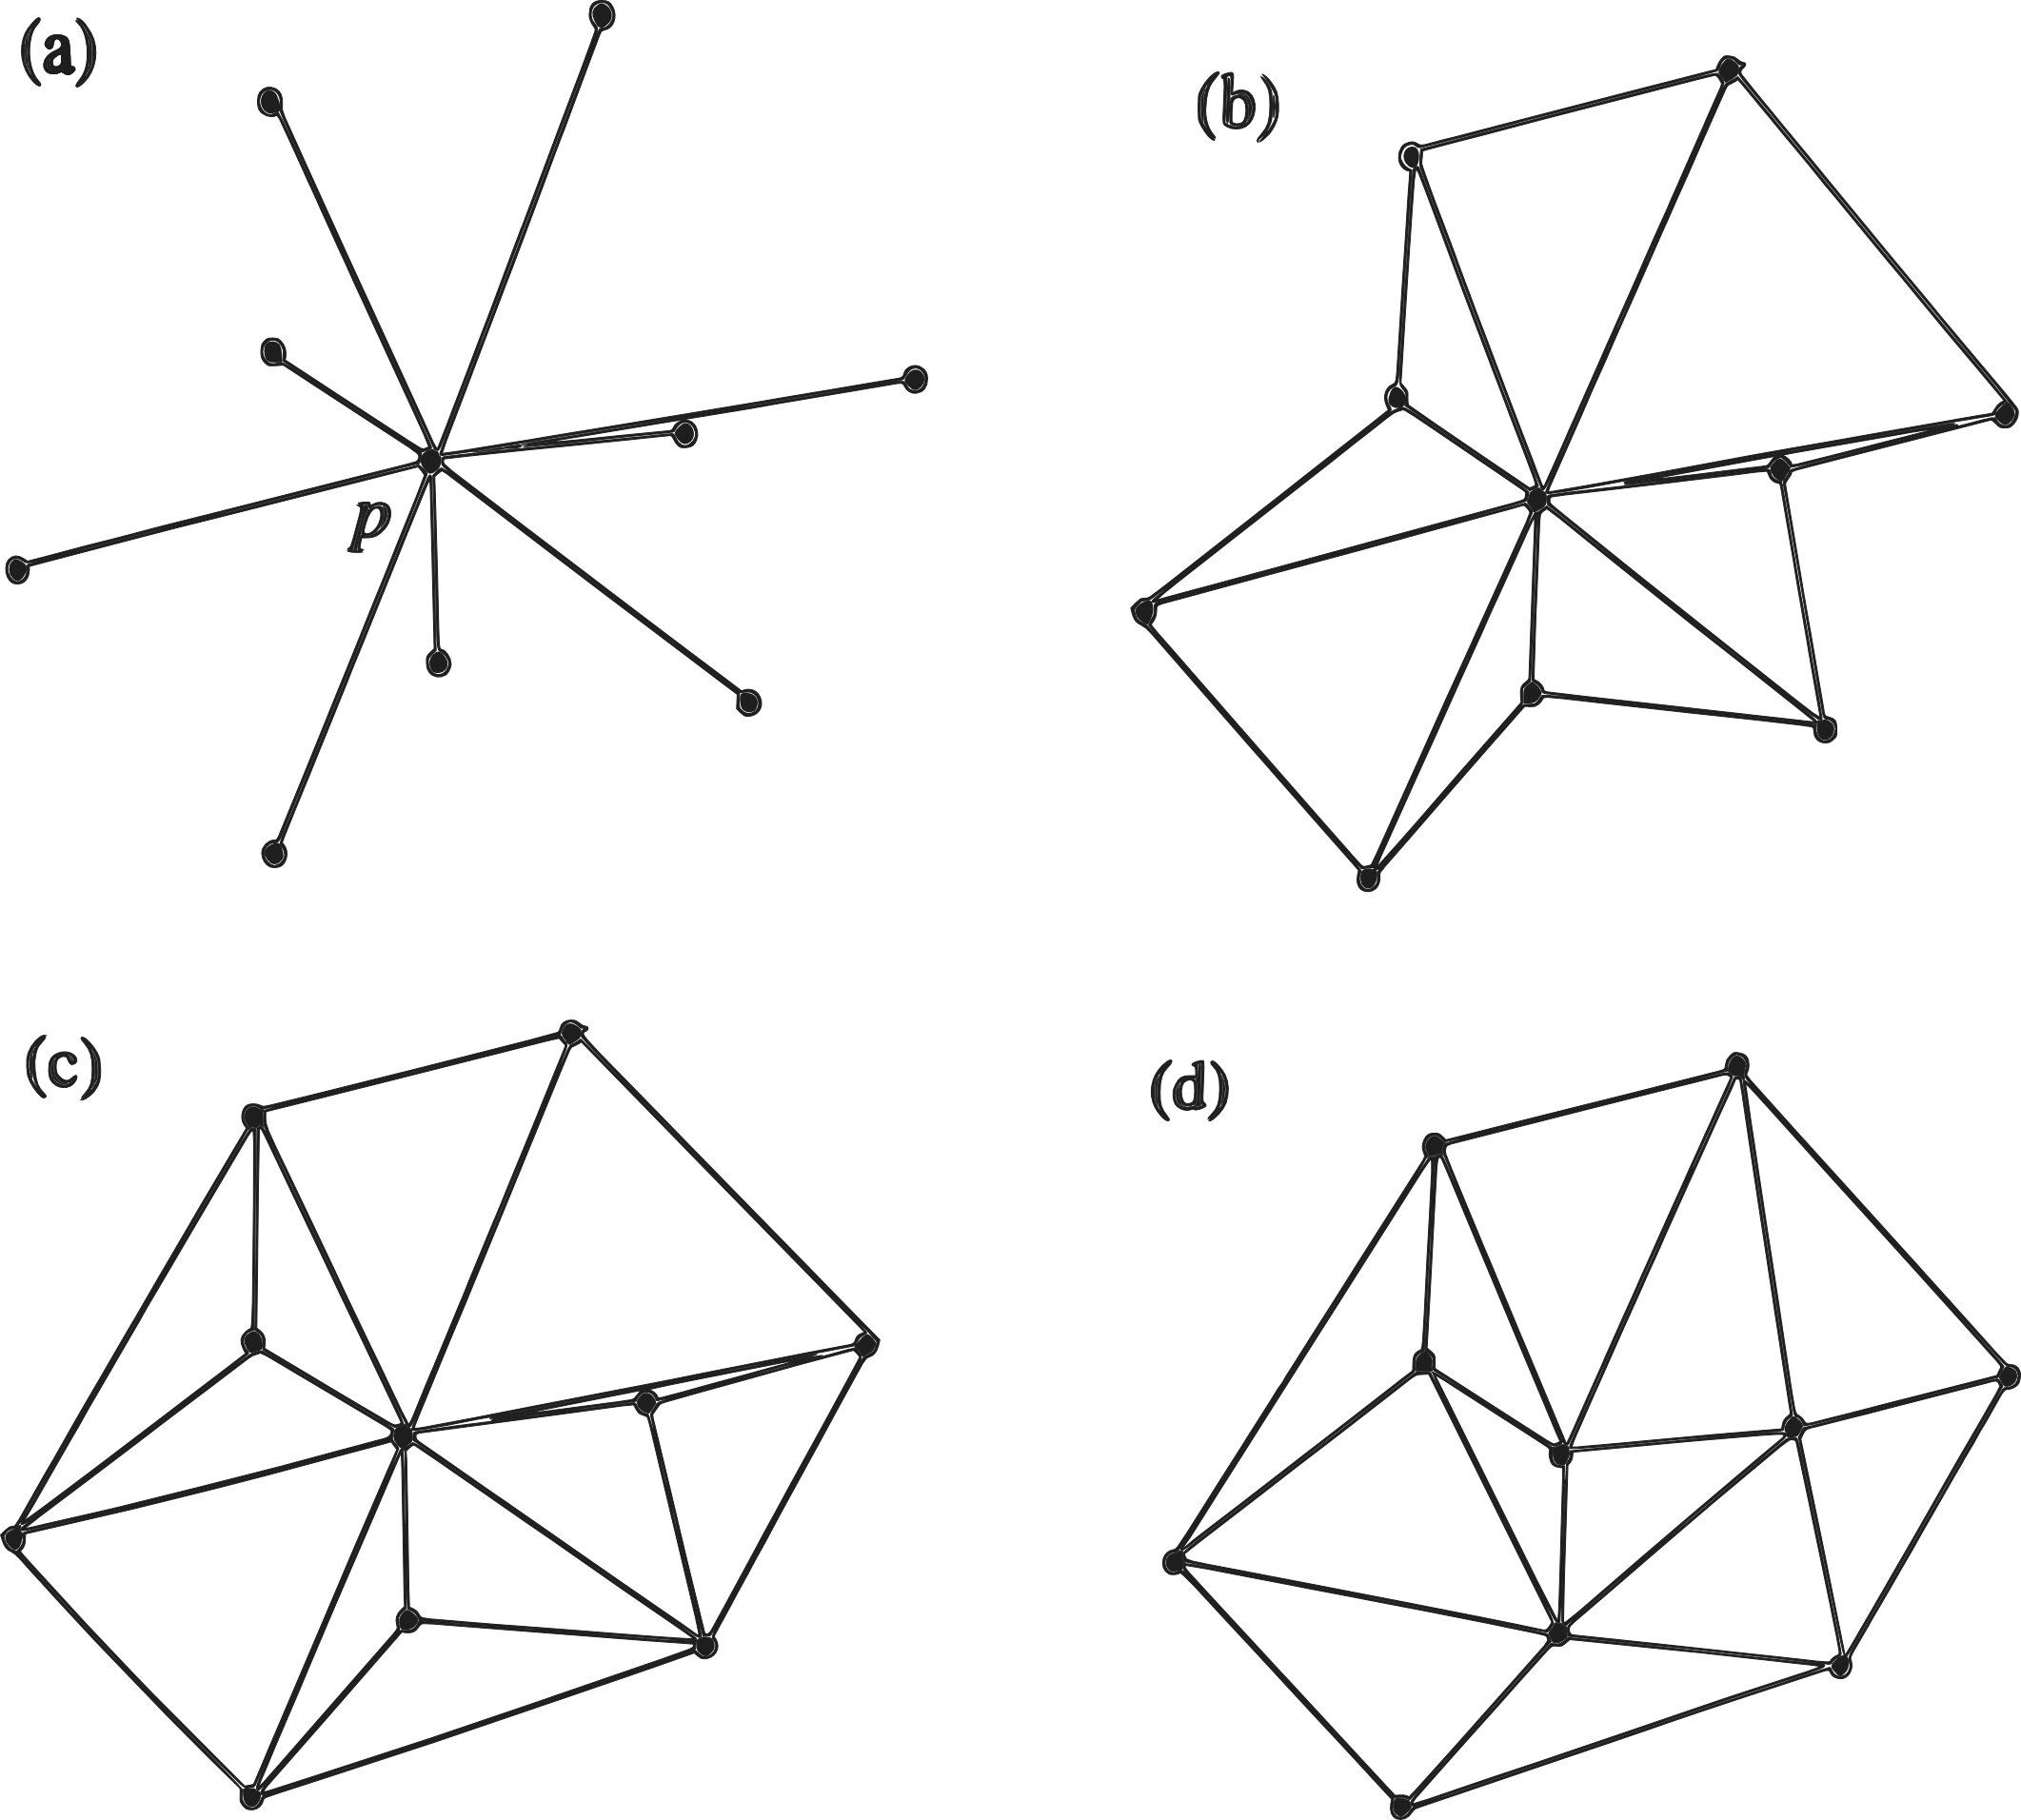
\includegraphics[width=0.85\textwidth]{img/rsweep.png}
\caption{Paprskovitý (Radial sweep) algoritmus, zdroj: \cite{triangulation}}
\label{fig:rsweep}
\end{figure}

\newpage
\subsection{Algoritmus inkrementálního vkládání}
\label{subsec:Inc_alg}

Tento algoritmus je poměrně jednoduchý a snadný na implementaci,
obzvlášť pokud je zvolena vhodná datová struktura. Jeho složitost je
$O(n^2)$, kterou lze úpravami zlepšit až na $O(n.log(n))$. Tato
metoda je tvořena třemi kroky. Na začátku je vytvořen konvexní obal
množiny bodů $P$ a pro jeho lomové body se provede triangulace. Do
vzniklé triangulace se postupně vkládají body z množiny $P$. Tato nově
vzniklá triangulace nemusí být nutně DT a proto se provede ještě její
legalizace.

\begin{algorithm}
\caption{Incremental algorithm}
\begin{algorithmic}[1]
\State Vytvoření konvexního obalu $\Omega$ nad množinou bodů $P$
\State Vytvoř DT pro lomové body konvexního obalu
\For{$i \in 1,...,n$}
	\State Přidej p do DT
	\State Najdi trojúhelník $t$ s vrcholy $p_i, p_j, p_k$ takový, že $p \in t$
	\If {$p$ leží uvnitř $t$}
		\State Přidání hrany $\overline{p,p_i}$
		\State Přidání hrany $\overline{p,p_j}$
		\State Přidání hrany $\overline{p,p_k}$
		\State Legalizace hrany $p,\overline{p_i,p_j},t$
		\State Legalizace hrany $p,\overline{p_j,p_k},t$
		\State Legalizace hrany $p,\overline{p_k,p_l},t$
	\ElsIf {$p$ leží na hraně $p_i, p_j$ trojúhelníků $t_1, t_2$}
		\State Přidání hrany $\overline{p,p_i}$
		\State Přidání hrany $\overline{p,p_j}$
		\State Přidání hrany $\overline{p,p_k}$
		\State Přidání hrany $\overline{p,p_l}$
		\State Legalizace hrany $p,\overline{p_j,p_k},t$
		\State Legalizace hrany $p,\overline{p_k,p_i},t$
		\State Legalizace hrany $p,\overline{p_i,p_l},t$
		\State Legalizace hrany $p,\overline{p_l,p_j},t$
	\EndIf
\EndFor
\end{algorithmic}
\end{algorithm}

\newpage
\subsection{Algoritmus inkrementální konstrukce (Step-by-Step)}

Tento postup, který je založen na postupném přidávání bodů do již
vytvořené DT, tvoří triangulaci postupně, trojúhelník po
trojúhelníku. Na začátku jsou vybrány dva body $p_1, p_2$, které jsou
sami sobě Voronoiovými sousedy, a mezi nimi je vytvořena základní
Delaunayova hrana $e$. K této hraně $e$ se hledá další bod $p$ tak,
aby vyhovoval kruhové podmínce a který společně s hranou $e$ vytvoří
Delaunayův trojúhelník s vrcholy $p_1, p_2$ a $p$, který se zapíše do
DT. Každá Delaunayovská hrana je orientována, bod $p$ hledáme pouze
vlevo od ní. Pro konstrukci se používá modifikovaná datová struktura
AEL (Active Edge List). Obsahuje hrany $e$, ke kterým hledáme body
$p$, do struktury se neukládá topologický model, viz kapitola
\ref{sec:data_struct}.

Základní vlastnost toho postupu je, že se v každém kroku ke stávající
triangulaci připojí další bod a triangulaci tak rozšíří. Vznikající
triangulace je už v procesu tvoření Delaunayova a není tedy třeba
žádné následující optimalizace.

\begin{figure}[h!]
\centering
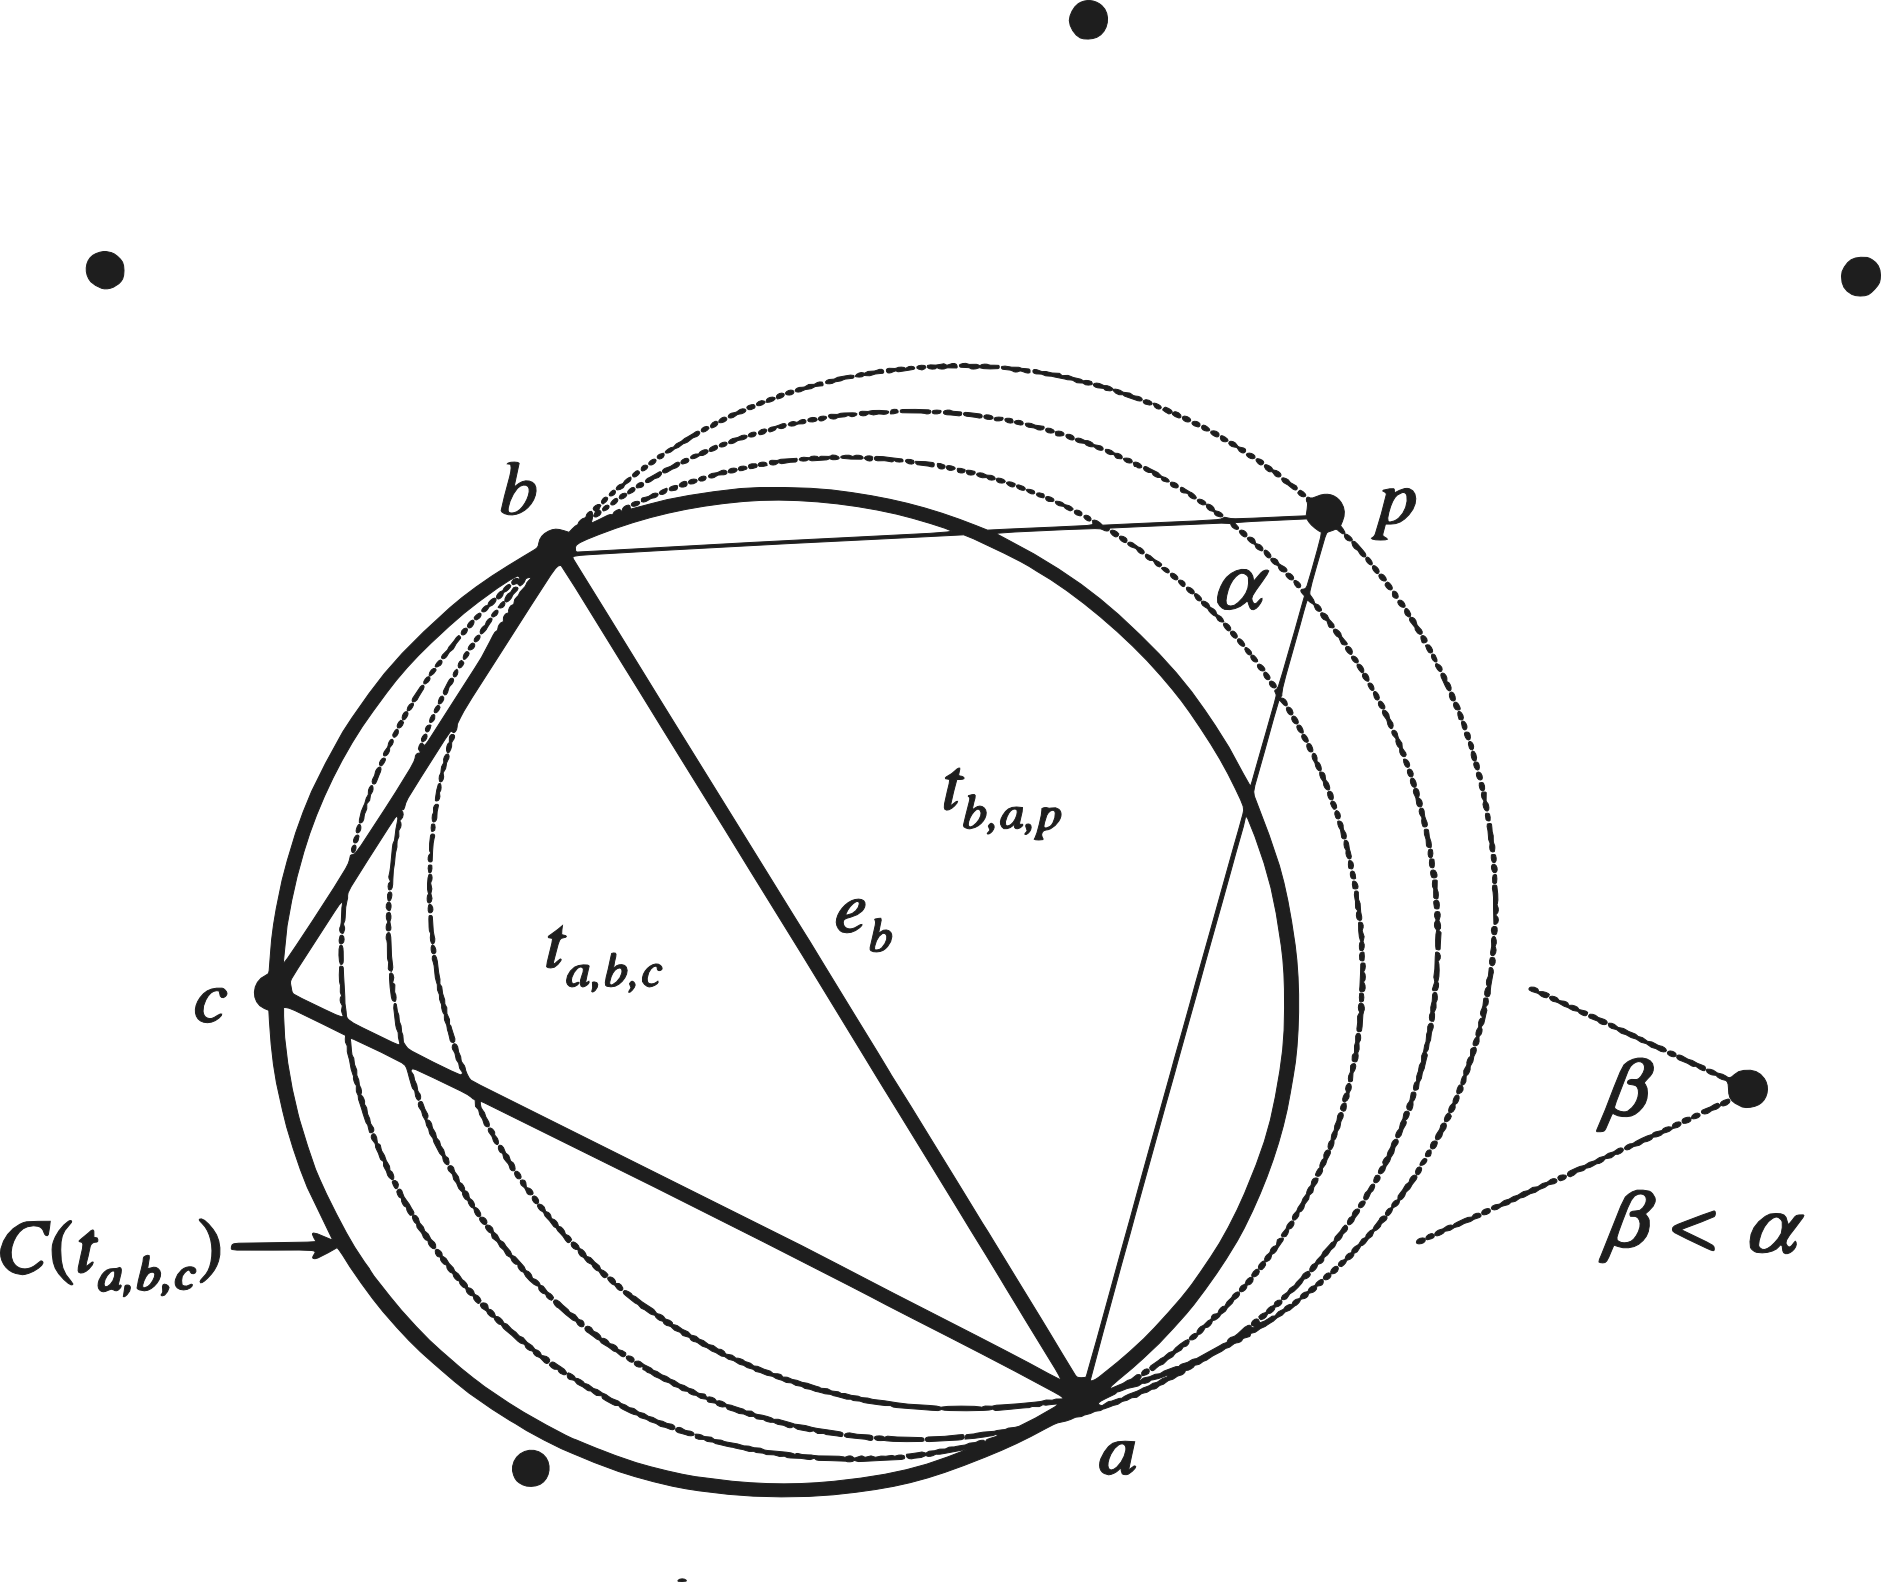
\includegraphics[width=0.7\textwidth]{img/stepbystep.png}
\caption{Algoritmus inkrementální konstrukce (Step-by-Step), zdroj: \cite{triangulation}}
\label{fig:stepbystep}
\end{figure}

%%% ML: tady nemas nektere veci prelozene (Add ... do)
%%% AL: prelozeno do cestiny
\newpage
\begin{algorithm}[h!]
\caption{Step-by-step algoritmus}
\begin{algorithmic}[1]
\State $p_1$=náhodný bod z $P$, $p_2$=nejbližší bod k $p_1$
\State Vytvoř hranu $\overline{e=p_1p_2}$
\State $p=d_D(e)$, bod s nejmenší Delaunay vzdáleností vlevo od $e$
\If{$p=NULL}$
	\State prohod’ orientaci $\overline{e=p_1p_2} \Rightarrow \overline{e=p_2p_1}$
\EndIf
\State $e_2=\overline{p_2p}$, $e_3=\overline{pp_1}$
\State  Přidej $e, e_2, e_3$ do AEL
\While {AEL není prázdný}
	\State $e=\overline{p_1p_2}$ první hrana AEL
	\State Změna orientace hrany $e=\overline{p_1p_2} \Rightarrow e=\overline{p_2p_1}$
	\State Bod $p$ s nejmenší Delaunay vzdáleností $d_D(e)$ vlevo od $e$
	\If {$p! =NULL$}
		\State $e_2=\overline{p_2p}, e_3=\overline{pp_1}$
		\State Přidej $e, e_2, e_3$ do AEL
		\State Přidej $e$ do DT
	\EndIf
	\State pop(e)
\EndWhile
\end{algorithmic}
\end{algorithm}

\newpage
\subsection{Algoritmus Rozděl a panuj}
\label{subsec:DnC_alg}

Rozděl a panuj (Divide and Conquer) je přístup, který vede k paralelizaci. Pro tvorbu
Delaunayovské triangulaci nabízí nejlepší výsledky, co se výkonnosti
týče. Tento přístup je založený na jednoduchých krocích:

\noindent 1. Rekurzivní dělení množiny bodů $P$ až do stavu, kdy se
pro podmnožinu nabízí jednoduché geometrické řešení. Při postupném
dělení množiny $P$ se nakonec dostaneme do stavu, kdy nám zbudou buď
tři body, v tom případě vytvoříme trojúhelník, nebo dva body, kdy
vytvoříme hranu.
\begin{figure}[h!]
\centering
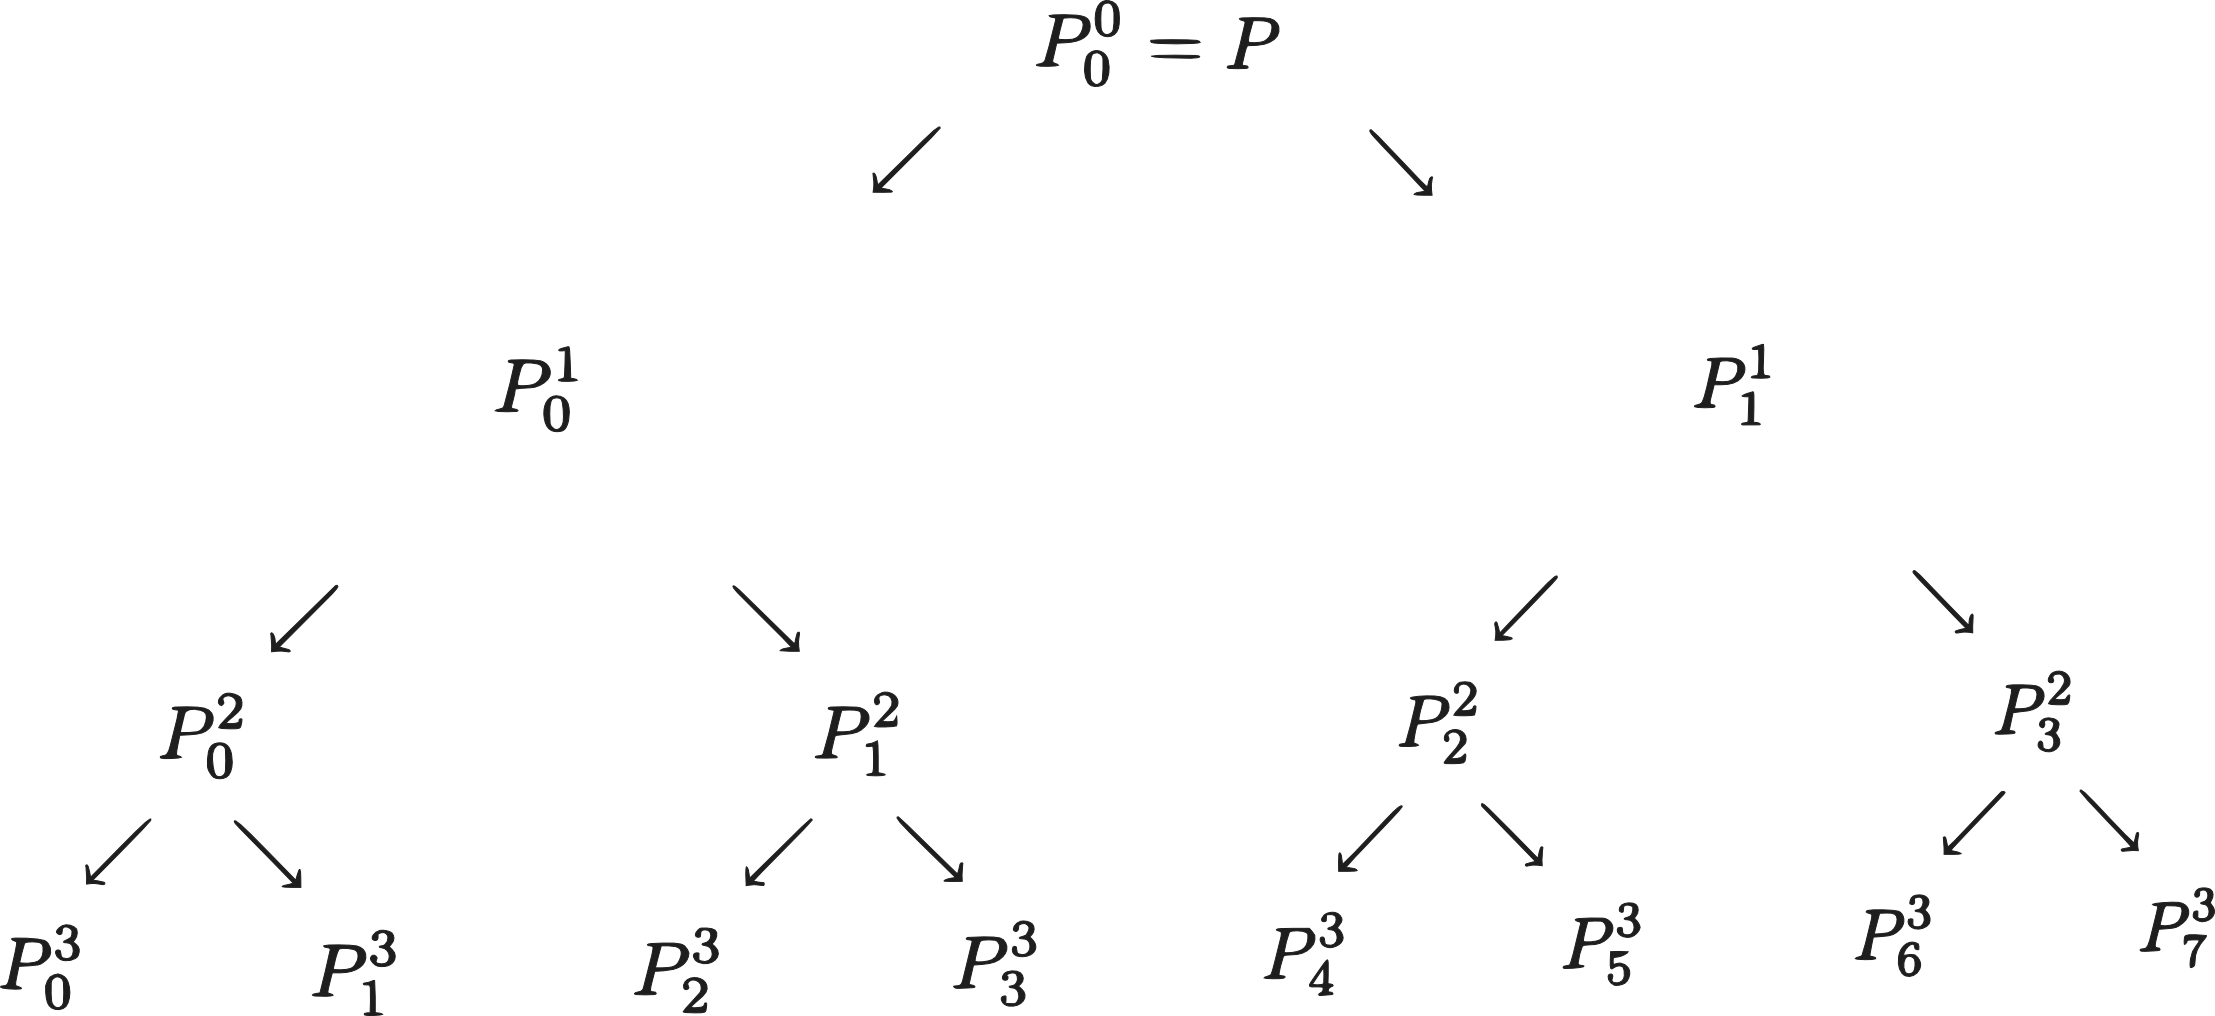
\includegraphics[width=0.65\textwidth]{img/div_n_conq.png}
\caption{Rekurzivní dělení na dílčí podmnožiny, zdroj: \cite{triangulation}}
\label{fig:div_n_conq}
\end{figure}

\noindent 2. Vytvoření prozatimní triangulace, která nemusí být
Delaunayovská.

\noindent 3. Připojení ke stávající triangulaci a její legalizace na
Delaunayovskou. Právě propojování podmnožin na jednotlivých vrstvách
je nejnáročnější část tohoto algoritmu.

\bigskip

%%% ML: dal jsem to na jednu stranku\newpage
\begin{figure}[h!]
\centering
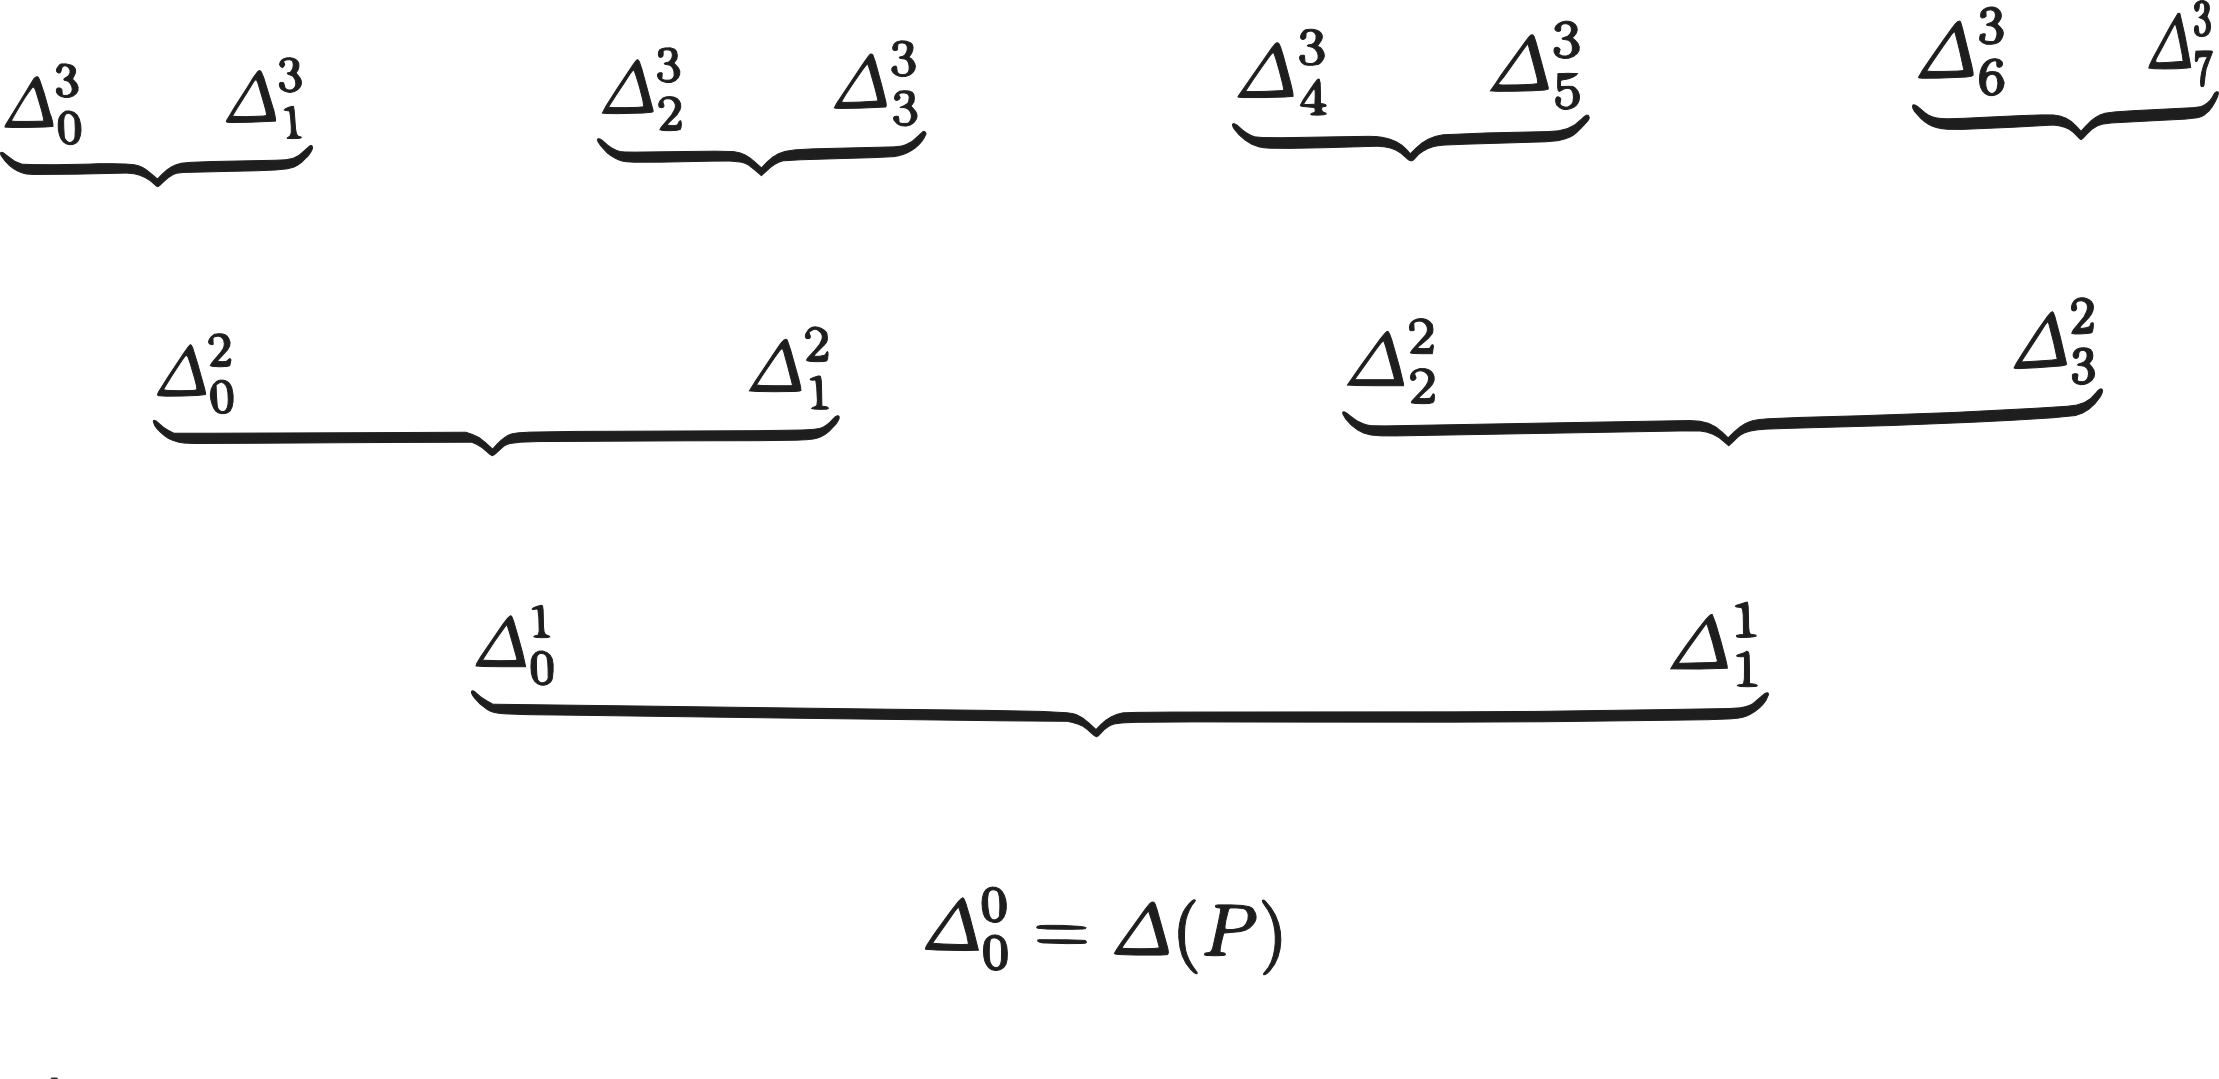
\includegraphics[width=0.65\textwidth]{img/merge.png}
\caption{Propojování dílčích triangulací, zdroj: \cite{triangulation}}
\label{fig:merge}
\end{figure}

%%% ML: tady pouzivas rovnou anglicky termin, predtim ho nemas uveden
%%% ani v zavorce
%%% AL: pouzit cesky termin, anglicky pridan do zavorky
Algoritmus Rozděl a panuj využívá GRASS modul \emph{v.delaunay}, o
kterém budeme mluvit později, viz kapitola \ref{subsec:v.delaunay}.


\newpage
\section{Datové struktury}
\label{sec:data_struct}

Existuje mnoho různých datových struktur pro uložení topologických
informací o triangulační síti. Každá nabízí nějaké výhody a uživatel
většinou musí řešit dva problémy. Jednak požadavky na dostatečnou
kapacitu pro uložení dat a pak dostatečnou efektivitu při získávání
informací ze struktury.

\begin{figure}[h!]
\centering
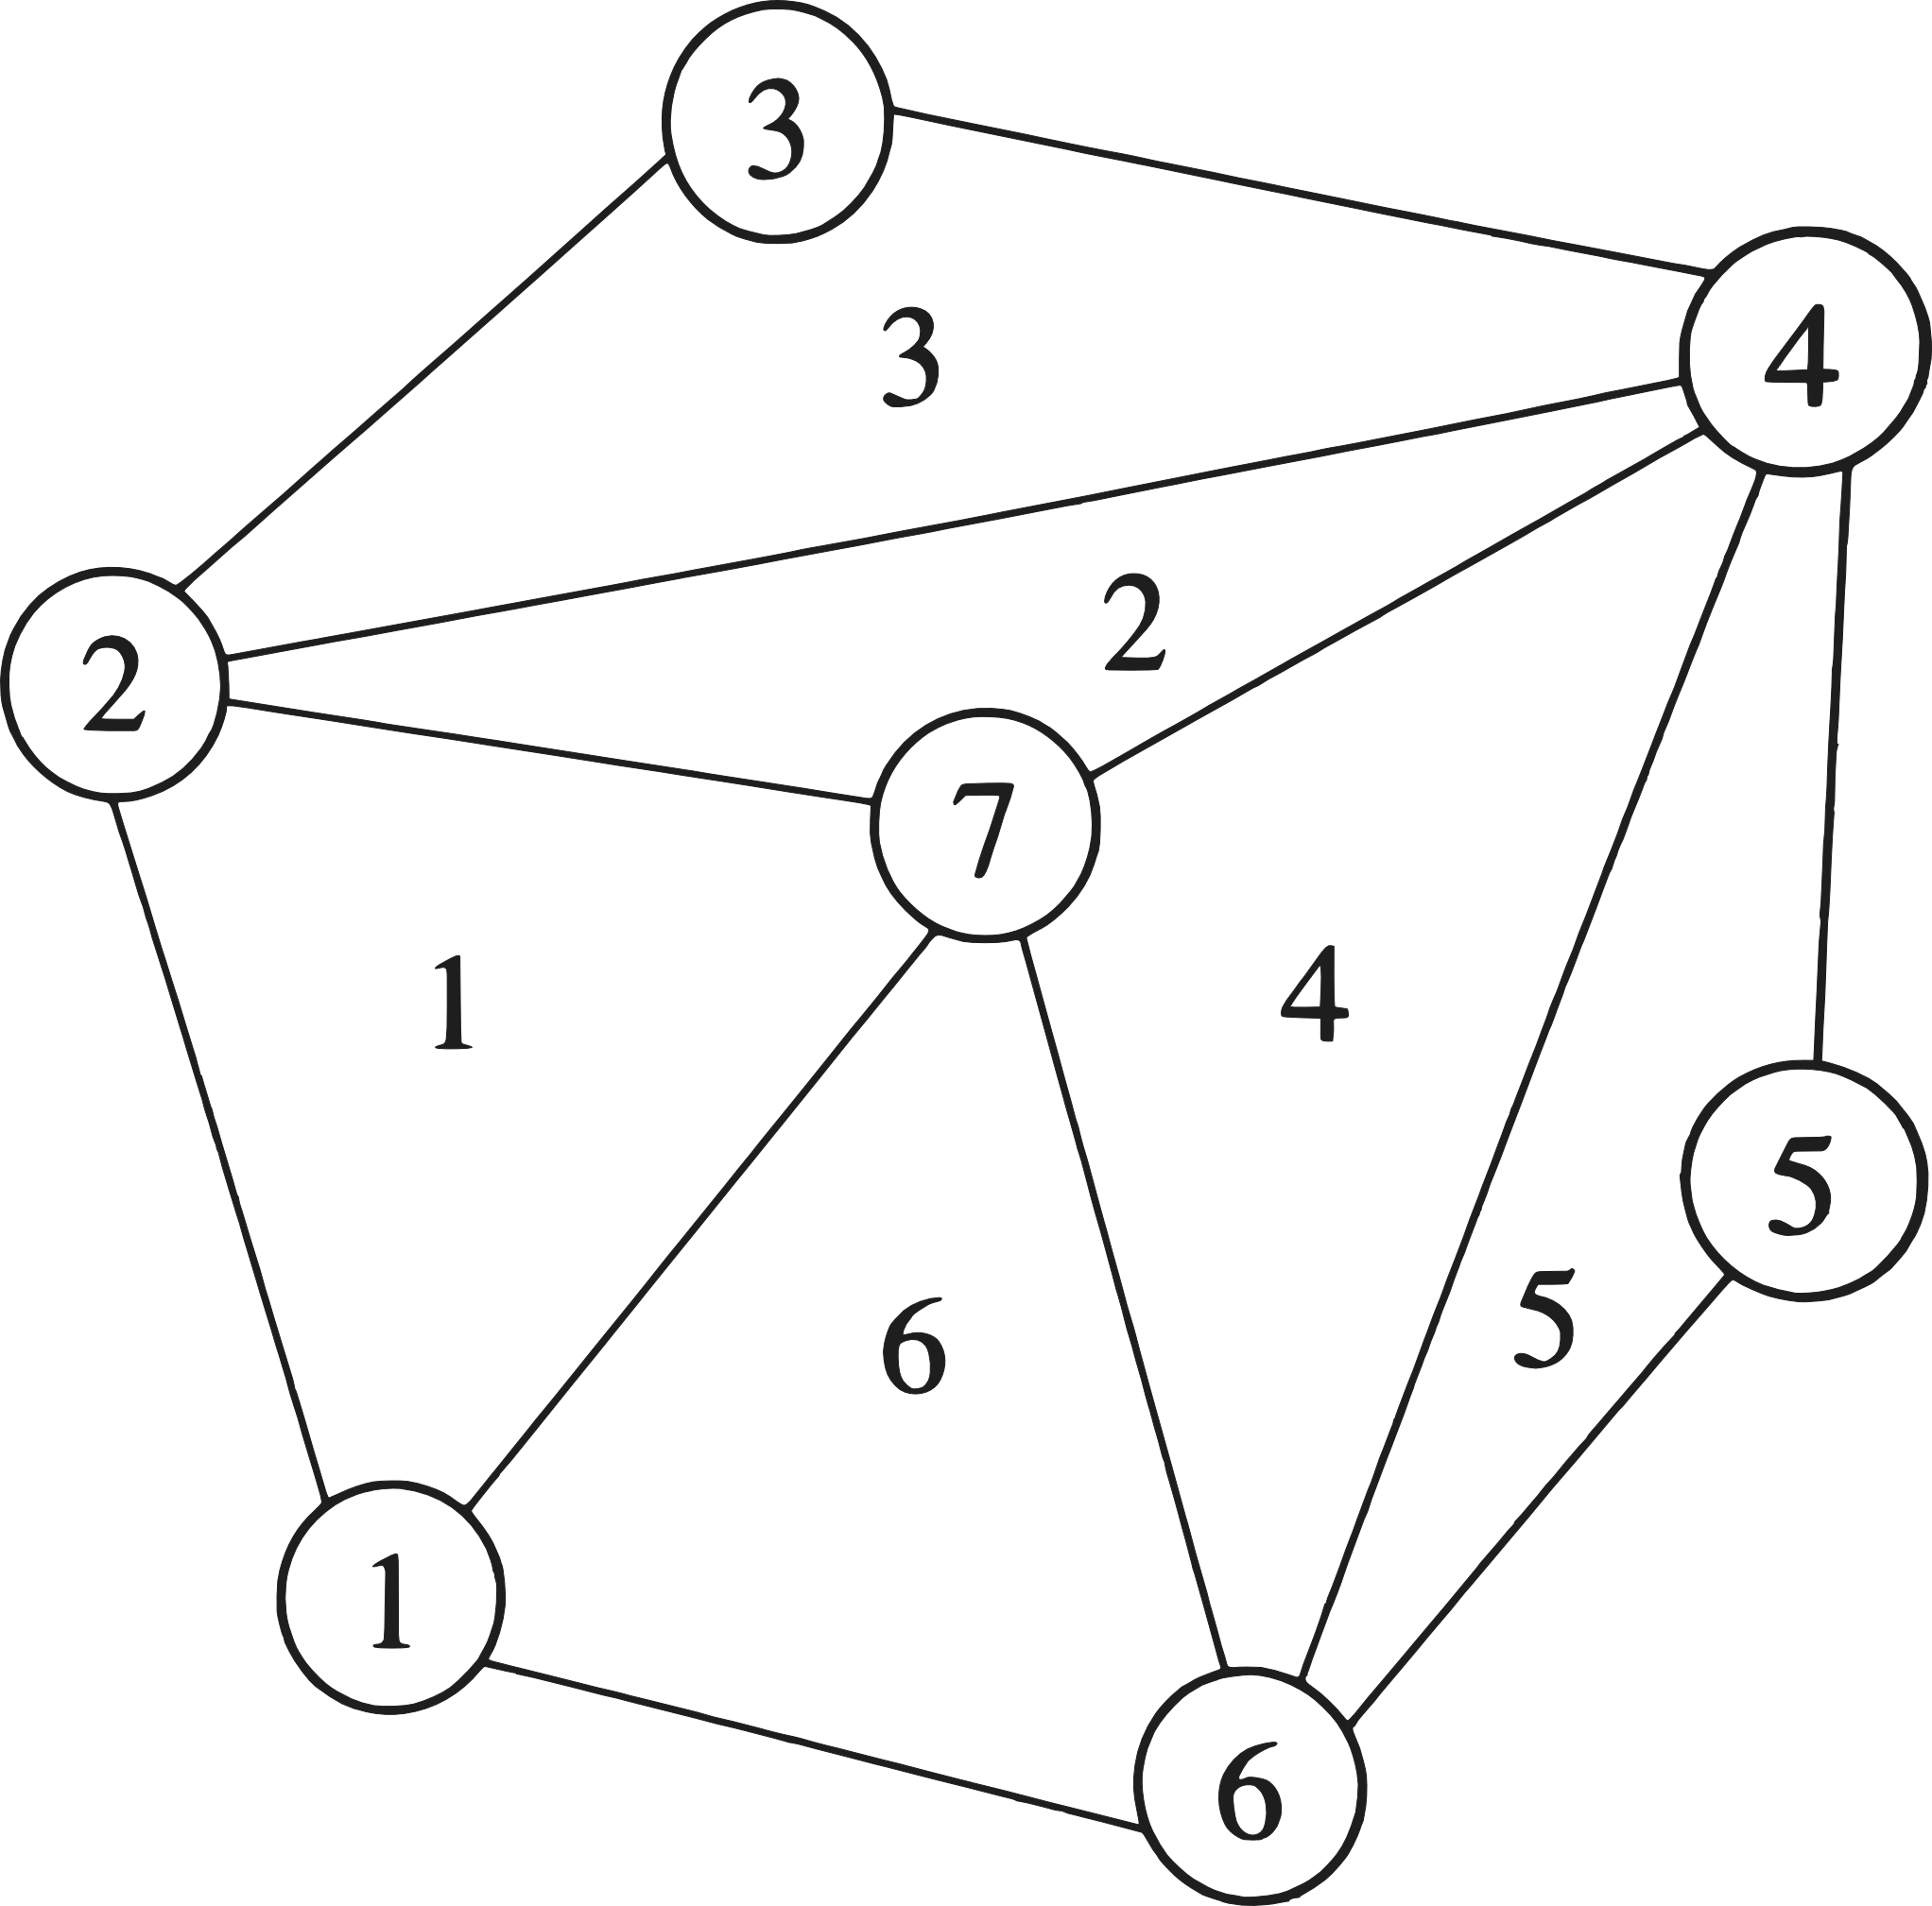
\includegraphics[width=0.6\textwidth]{img/data_struct.png}
\caption{Příklad jednoduché triangulace}
\label{fig:struct_triangulace}
\end{figure}

\newpage
\subsection{Jednoduchá trojúhelníková struktura}

Tato struktura ukládá informace v nejjednodušší podobě. Pracuje pouze
s trojicemi id jednotlivých vrcholů trojúhelníků v seznamu nebo v
poli. Trojúhelníky jsou seřazeny vzestupně podle id, zatímco na pořadí
uložených vrcholů nezáleží. Struktura je velmi nenáročná, co se
požadavků na kapacitu týče, nicméně toto je vykoupené tím, že nemáme k
dispozici žádnou informaci, který trojúhelník sousedí s kterým.

\begin{table}[h]
\catcode`\-=12
\begin{tabular}{|c||c|c|c|}
\hline
\multirow{2}{*}{Trojúhelník} & \multicolumn{3}{c|}{Vrcholy} \\ \cline{2-4} 
                             & i        & j       & k       \\ \hline \hline
1                            & 1        & 7       & 2       \\ \hline
2                            & 2        & 7       & 4       \\ \hline
3                            & 2        & 4       & 3       \\ \hline
4                            & 7        & 6       & 4       \\ \hline
5                            & 4        & 6       & 5       \\ \hline
6                            & 7        & 1       & 6       \\ \hline
\end{tabular}
\caption{Jednoduchá trojúhelníková struktura}
\label{tab:troj_struktura_simple}
\end{table}



\subsection{Trojúhelníková struktura se sousedy}

Tato struktura přináší rozšíření o informaci, s kterými trojúhelníky
daný trojúhelník sousedí. K zapotřebí je tedy další seznam, který
obsahuje id trojúhelníku.

\begin{table}[h]
\catcode`\-=12
\begin{tabular}{|c||c|c|c||c|c|c|}
\hline
\multirow{2}{*}{Trojúhelník} & \multicolumn{3}{|c|}{Vrcholy} & \multicolumn{3}{|c|}{Sousedé}      \\ \cline{2-7} 
                             & i        & j       & k       & $t_{j,k}$ & $t_{k,i}$ & $t_{i,j}$ \\ \hline \hline
1                            & 1        & 7       & 2       & 2         & -         & 6         \\ \hline
2                            & 2        & 7       & 4       & 4         & 3         & 1         \\ \hline
3                            & 2        & 4       & 3       & -         & -         & 2         \\ \hline
4                            & 7        & 6       & 4       & 5         & 2         & 6         \\ \hline
5                            & 4        & 6       & 5       & -         & -         & 4         \\ \hline
6                            & 7        & 1       & 6       & -         & 4         & 1         \\ \hline
\end{tabular}
\caption{Trojúhelníková struktura se sousedy}
\label{tab:troj_strukt_sous}
\end{table}

\subsection{Vertex-based struktura se sousedy}

Vertex-based struktura se sousedy je poměrně úsporná struktura, co se
objemu dat týče. Ke každému vrcholu $v_i$ v síti jsou uloženy do
seznamu sousedů vrcholy, které jsou s ním spojené. V případě, že $v_i$
leží na konvexním obalu je seznam sousedů ukončen 'pseudo-vrcholem'.

\begin{table}[h]
\catcode`\-=12
\begin{tabular}{|c||c|c|c|c|c|c||c|}
\hline
Vrchol & \multicolumn{6}{|c|}{Sousední vrcholy} & Suma vrcholů \\ \hline \hline
1      & 6    & 7    & 2    & 0    &     &     & 4            \\ \hline
2      & 1    & 7    & 4    & 3    & 0   &     & 9            \\ \hline
3      & 2    & 4    & 0    &      &     &     & 12           \\ \hline
4      & 3    & 2    & 7    & 6    & 5   & 0   & 18           \\ \hline
5      & 4    & 6    & 0    &      &     &     & 21           \\ \hline
6      & 5    & 4    & 7    & 1    & 0   &     & 26           \\ \hline
7      & 6    & 4    & 2    & 1    &     &     & 30           \\ \hline
\end{tabular}
\caption{Vertex based struktura}
\label{tab:vertex_based}
\end{table}

\begin{figure}[h!]
\centering
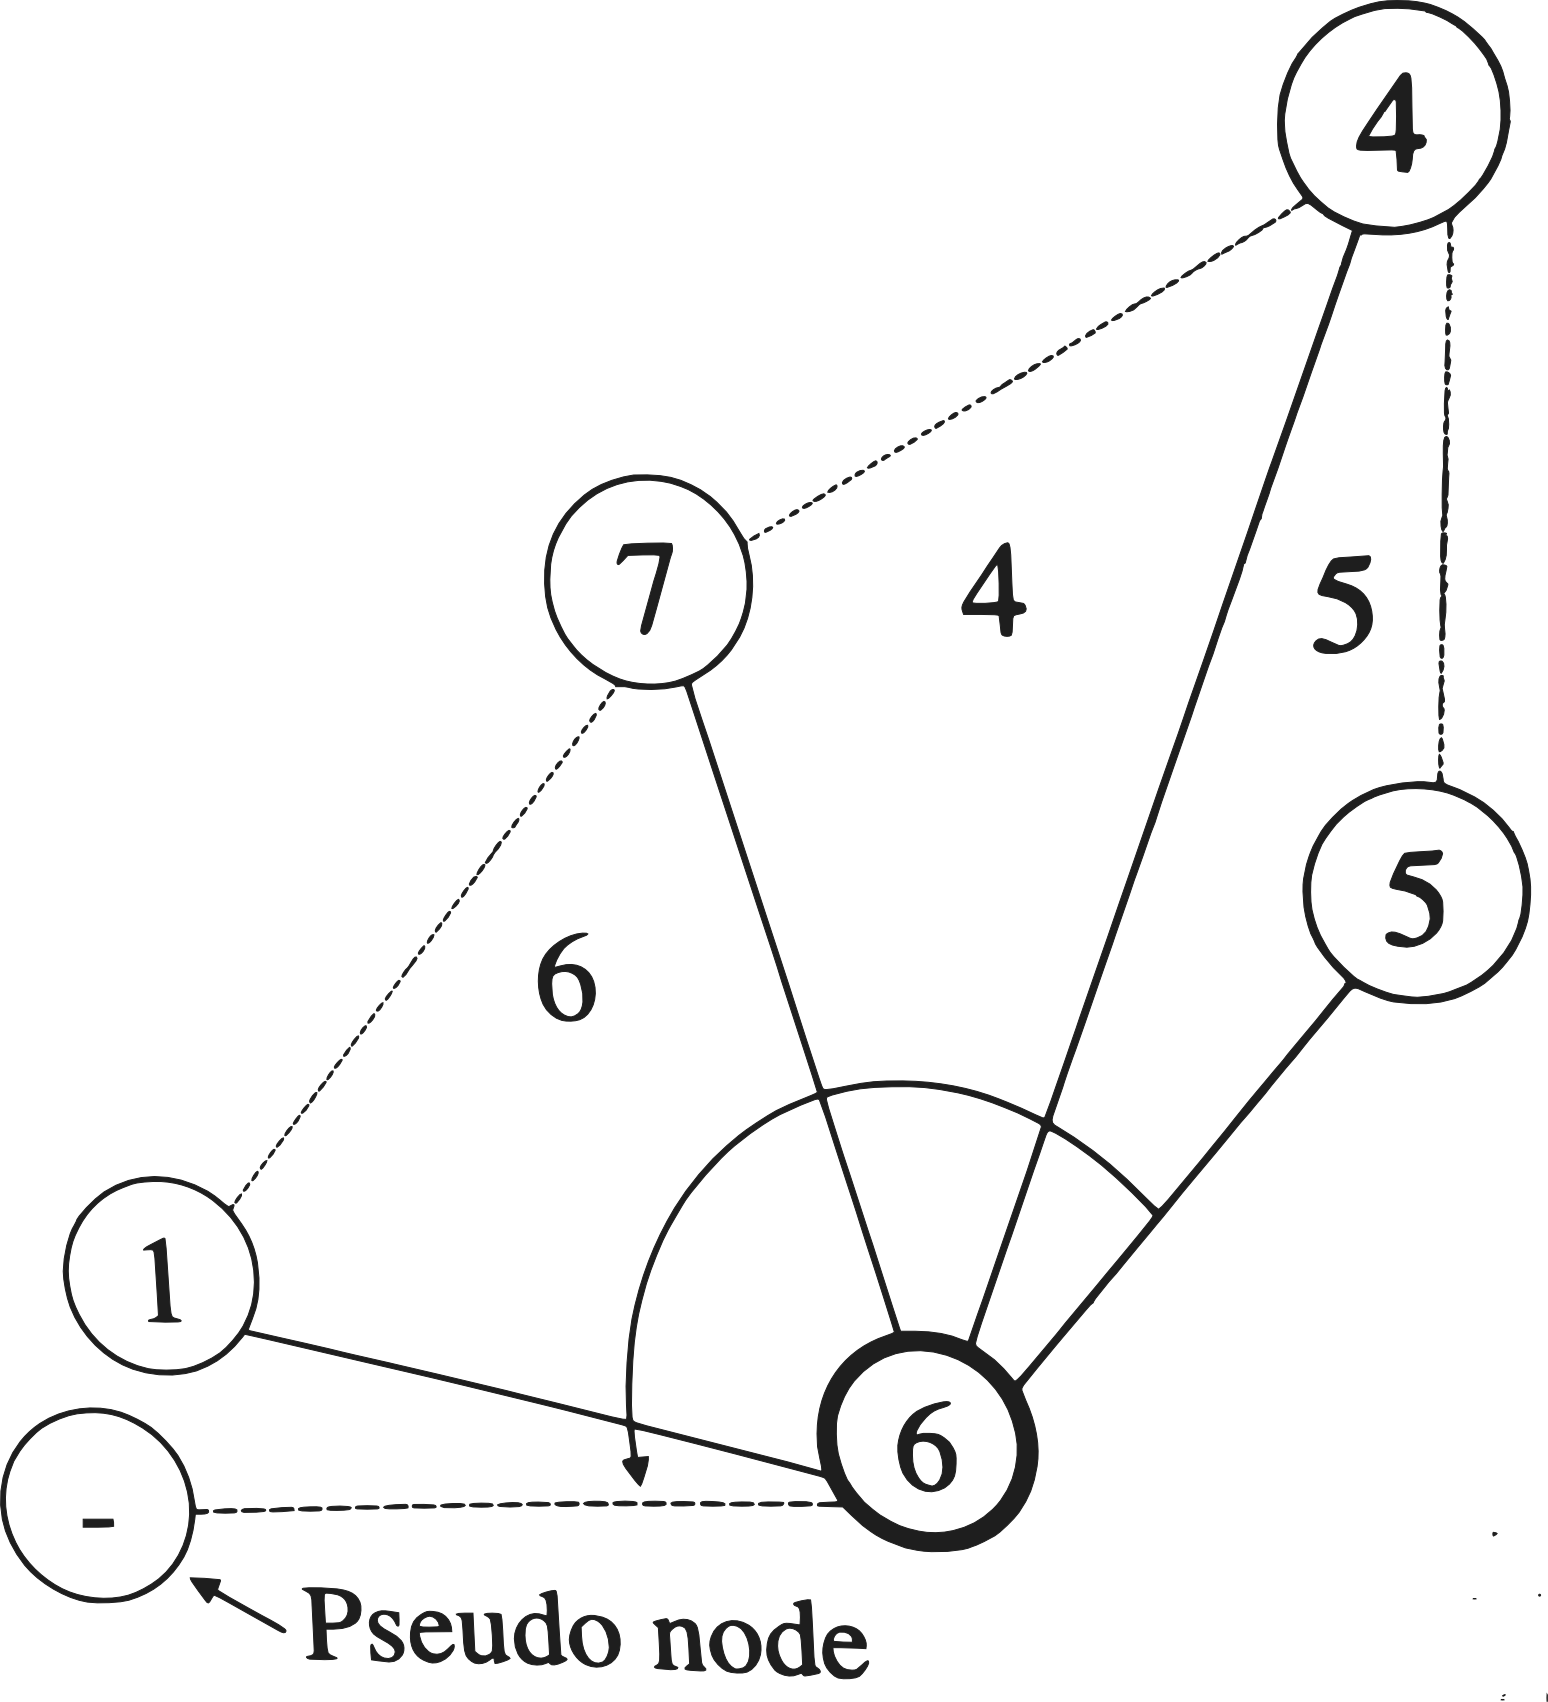
\includegraphics[width=0.4\textwidth]{img/pseudo_node.png}
\caption{Datová struktura s použitím pseudo-uzlu, zdroj: \cite{triangulation}}
\label{fig:pseudo_node}
\end{figure}

\newpage
\subsection{Half-edge datová struktura}
\label{subsec:HE_struct}

Tato struktura uchovává topologický model na základě orientovaných
polovičních hran. Princip je rozdělit každou hranu na dvě orientované
\emph{půlhrany}, z nichž každá směřuje opačným směrem. Každému
trojúhelníku můžeme tak přiřadit tři půlhrany, které jsou orientované
v protisměru hodinových ručiček. Každá půlhrana začíná
v~\emph{počátečním vrcholu} a směřuje do \emph{cílového vrcholu}. V
%%% ML: misto poiter spise ukazatel - detail
%%% AL:opraveno
half-edge struktuře si každá půlhrana uchovává ukazatel na svůj
počáteční bod, na svůj koncový bod, na předchozí i následující
půl-hranu, patřící stejnému trojúhelníku a nakonec pointer na opačně
orientovanou hranu, tzv. \emph{twin-edge}. Pointer na twin-edge hranu
%%% ML: pomlcka pul-hrana nepusobi prilis cesky, lepe vypada
%%% "pulhrana", otrocky prepisovat z anglictiny neni nutne - detail
%%% AL: prepsano na pulhrana
nemají pouze půlhrany ležící na konvexním obalu triangulace.

\begin{figure}[h!]
\centering
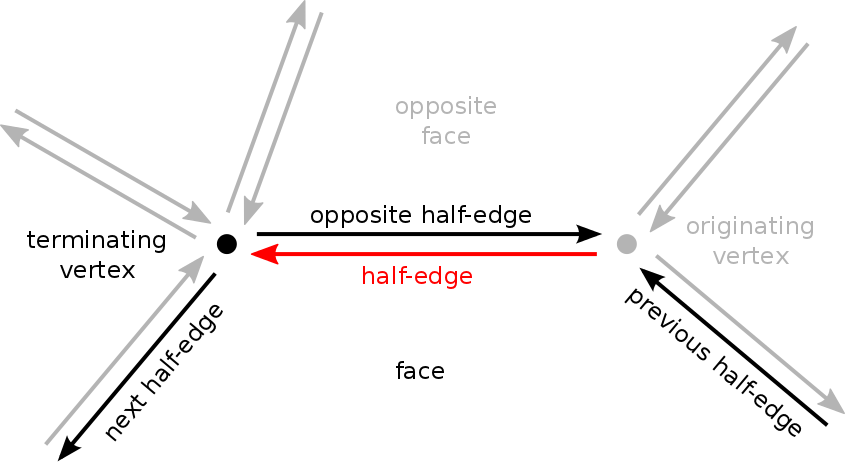
\includegraphics[width=0.9\textwidth]{img/half_edge.png}
\caption{Half-edge struktura (Zdroj: \url{http://pointclouds.org/blog/nvcs/martin/index.php})}
\label{fig:half_edge}
\end{figure}

Z half-edge struktury je možné odvodit mnohé jiné příbuzné struktury
obsahující další informace o topologii, které ulehčují procházení
celou sítí při vyhledávání, ale zároveň zvyšují nároky na
kapacitu. Mezi tyto příbuzné struktury patří například
\emph{vertex-edge}, \emph{face-edge} nebo \emph{winged edge} datová
struktura, kterou používá například modul \emph{v.delaunay} v GRASS
GISu, kapitola \ref{subsec:v.delaunay}.

\newpage
\begin{figure}[h!]
\centering
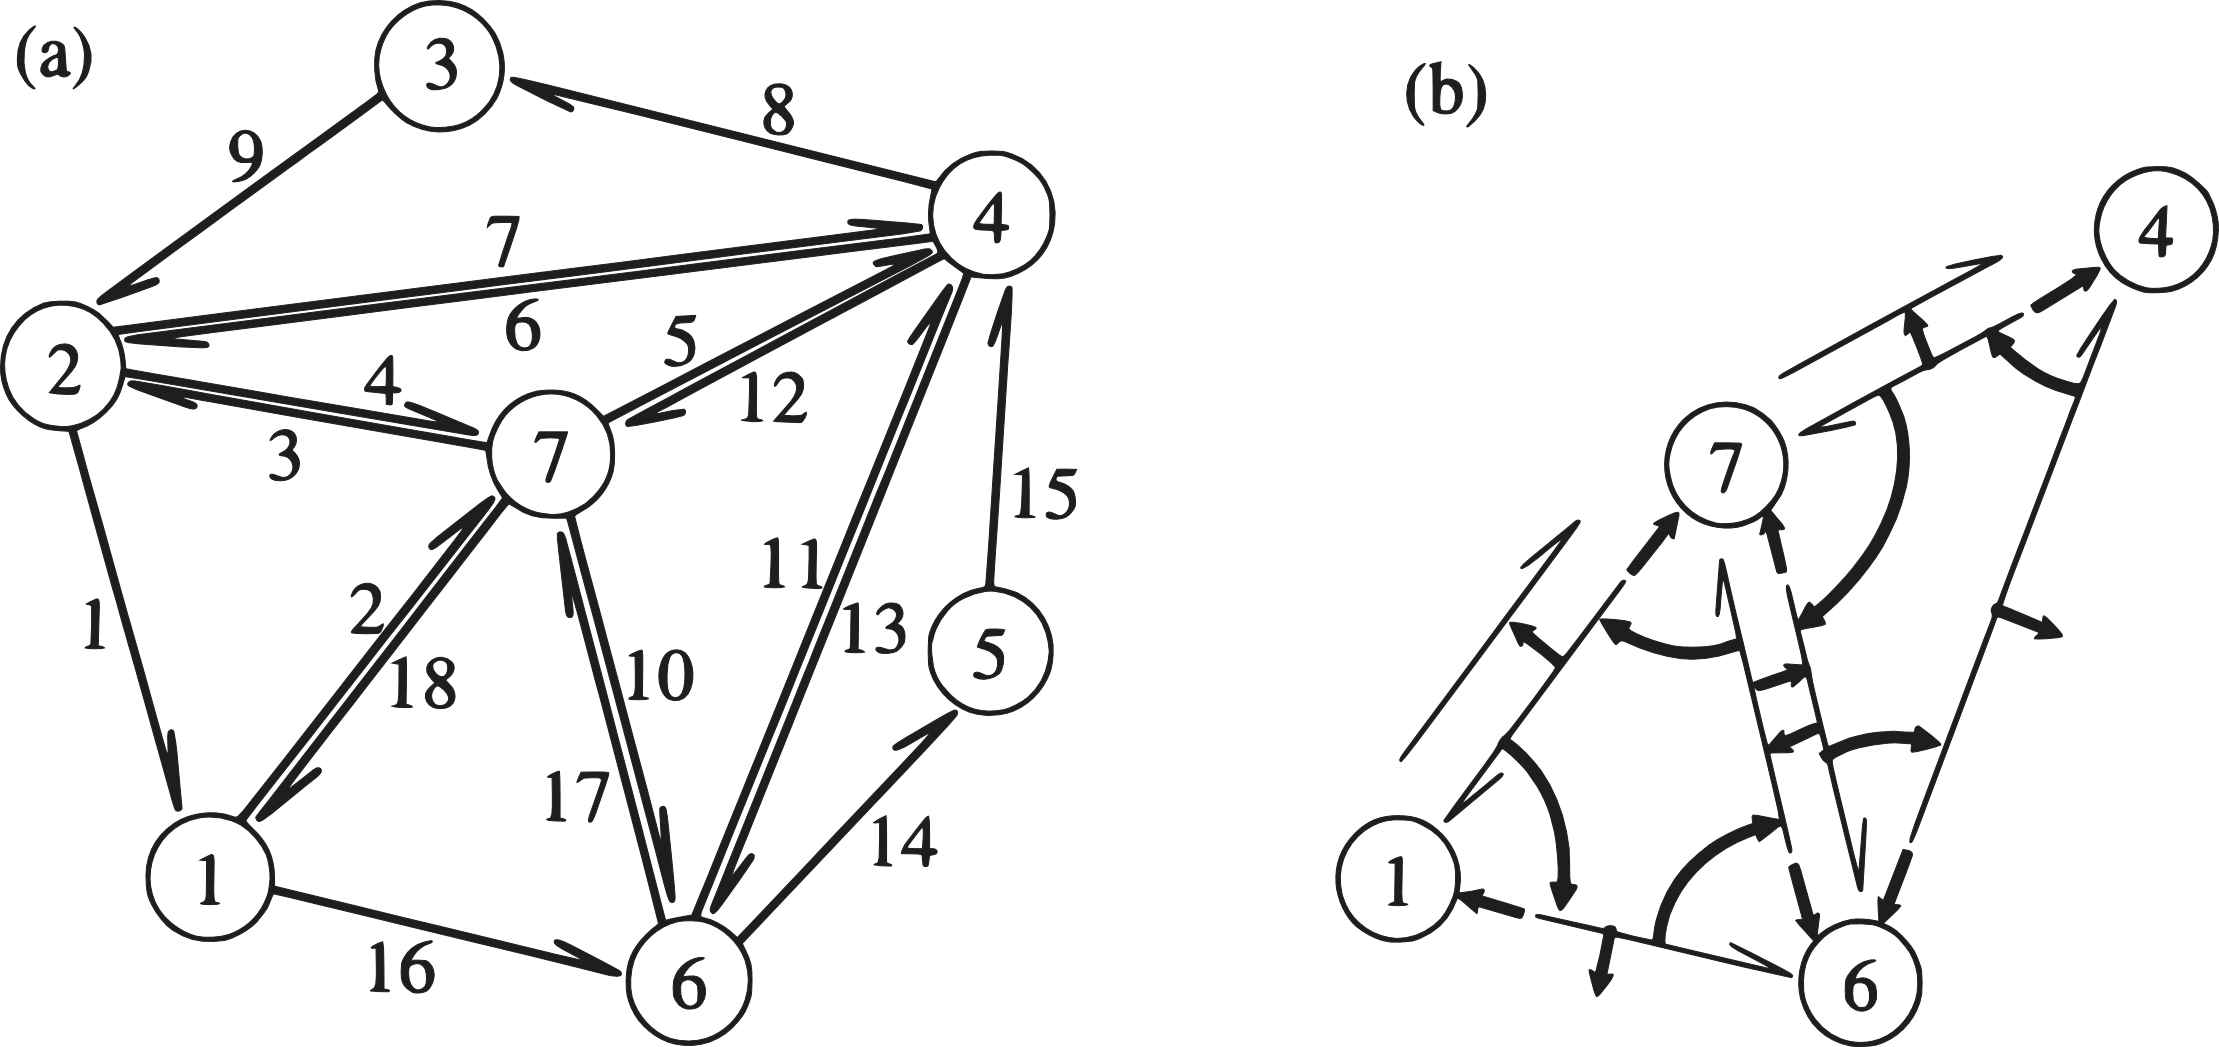
\includegraphics[width=0.8\textwidth]{img/half_edge2.png}
\caption{Half-edge struktura, zdroj: \cite{triangulation}}
\label{fig:half_edge_scan}
\end{figure}
\begin{table}[h!]
\catcode`\-=12
\begin{tabular}{|c||c||c|c|}
\hline
\multirow{2}{*}{Půl-hrana} & \multirow{2}{*}{Startovní vrchol} & \multicolumn{2}{c|}{Half-edge pointry} \\ \cline{3-4} 
                           &                                   & Další hrana v trojúhelníku & Twin-edge \\ \hline
1                          & 2                                 & 2                          & -         \\ \hline
2                          & 1                                 & 3                          & 18        \\ \hline
3                          & 7                                 & 1                          & 4         \\ \hline
4                          & 2                                 & 5                          & 3         \\ \hline
5                          & 7                                 & 6                          & 12        \\ \hline
6                          & 4                                 & 4                          & 7         \\ \hline
7                          & 2                                 & 8                          & 6         \\ \hline
8                          & 4                                 & 9                          & -         \\ \hline
9                          & 3                                 & 7                          & -         \\ \hline
10                         & 7                                 & 11                         & 17        \\ \hline
11                         & 6                                 & 12                         & 13        \\ \hline
12                         & 4                                 & 10                         & 5         \\ \hline
13                         & 4                                 & 14                         & 11        \\ \hline
14                         & 6                                 & 15                         & -         \\ \hline
15                         & 5                                 & 13                         & -         \\ \hline
16                         & 1                                 & 17                         & -         \\ \hline
17                         & 6                                 & 18                         & 10        \\ \hline
18                         & 7                                 & 16                         & 2         \\ \hline
\end{tabular}
\caption{Half-edge struktura}
\label{tab:half_edge}
\end{table}

\newpage
\begin{lstlisting}[caption={Definice datové struktury}]
class Half-edge
{
	Point *originating_vertex;
	Half-edge *edge, *next_edge, *twin_edge;
	
};
\end{lstlisting}

\subsection{Dart-based datová struktura}

Dart-based datová struktura nabízí extrémně rychlé procházení
topologie napříč datovou strukturou. Ta může být representována jako
množina ukazatelů, tzv. \emph{dartů} $D$. Dart $d \in D$ představuje
trojici $(v_i, e_j, t_k)$, kde $v_i$ je vrchol hrany $e_j$ v
trojúhelníku $t_k$. V jednom trojúhelníky tedy můžeme definovat celkem
šest dartů. Každý dart $d \in D$ odkazuje k jednomu vrcholu a třem
dalším dartům z $D$ pomocí takzvaných $\alpha$\emph{- iteratorů}. Tyto
iterátory jsou definovány takto (obrázek \ref{fig:iterators}(b)):
\begin{itemize}
\item $\alpha_0(d)$ odkazuje k trojici s rozdílným vrcholem $v$, ale stejnou hranou $e$ a trojúhelníkem $t$,
\item $\alpha_1(d)$ odkazuje k trojici s rozdílnou hranou $e$, ale stejným vrcholem $v$ a trojúhelníkem $t$,
\item $\alpha_2(d)$ odkazuje k trojici s rozdílným trojúhelníkem $t$, ale stejným vrcholem $v$ a hranou $e$.
\end{itemize}

\begin{figure}[h!]
\centering
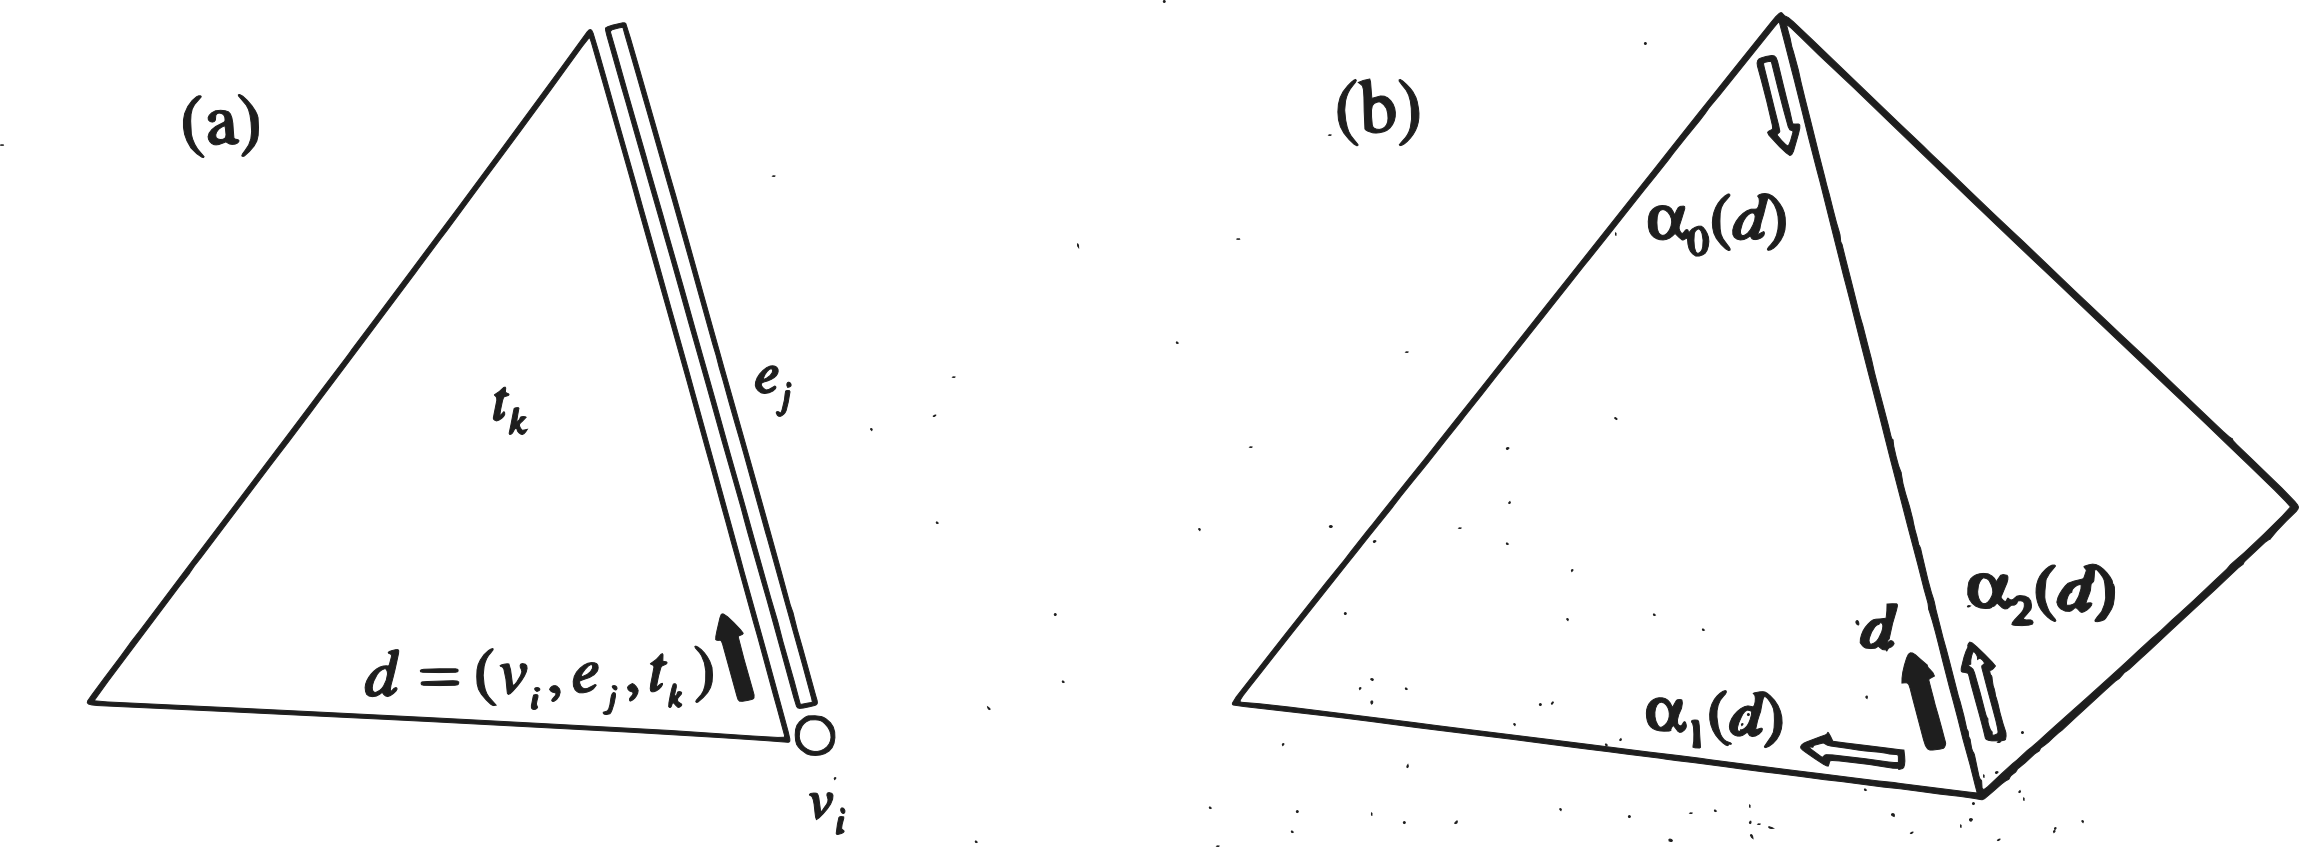
\includegraphics[width=0.8\textwidth]{img/iterators.png}
\caption{$\alpha-iterátory $, zdroj: \cite{triangulation}}
\label{fig:iterators}
\end{figure}

\newpage
\begin{figure}[h!]
\centering
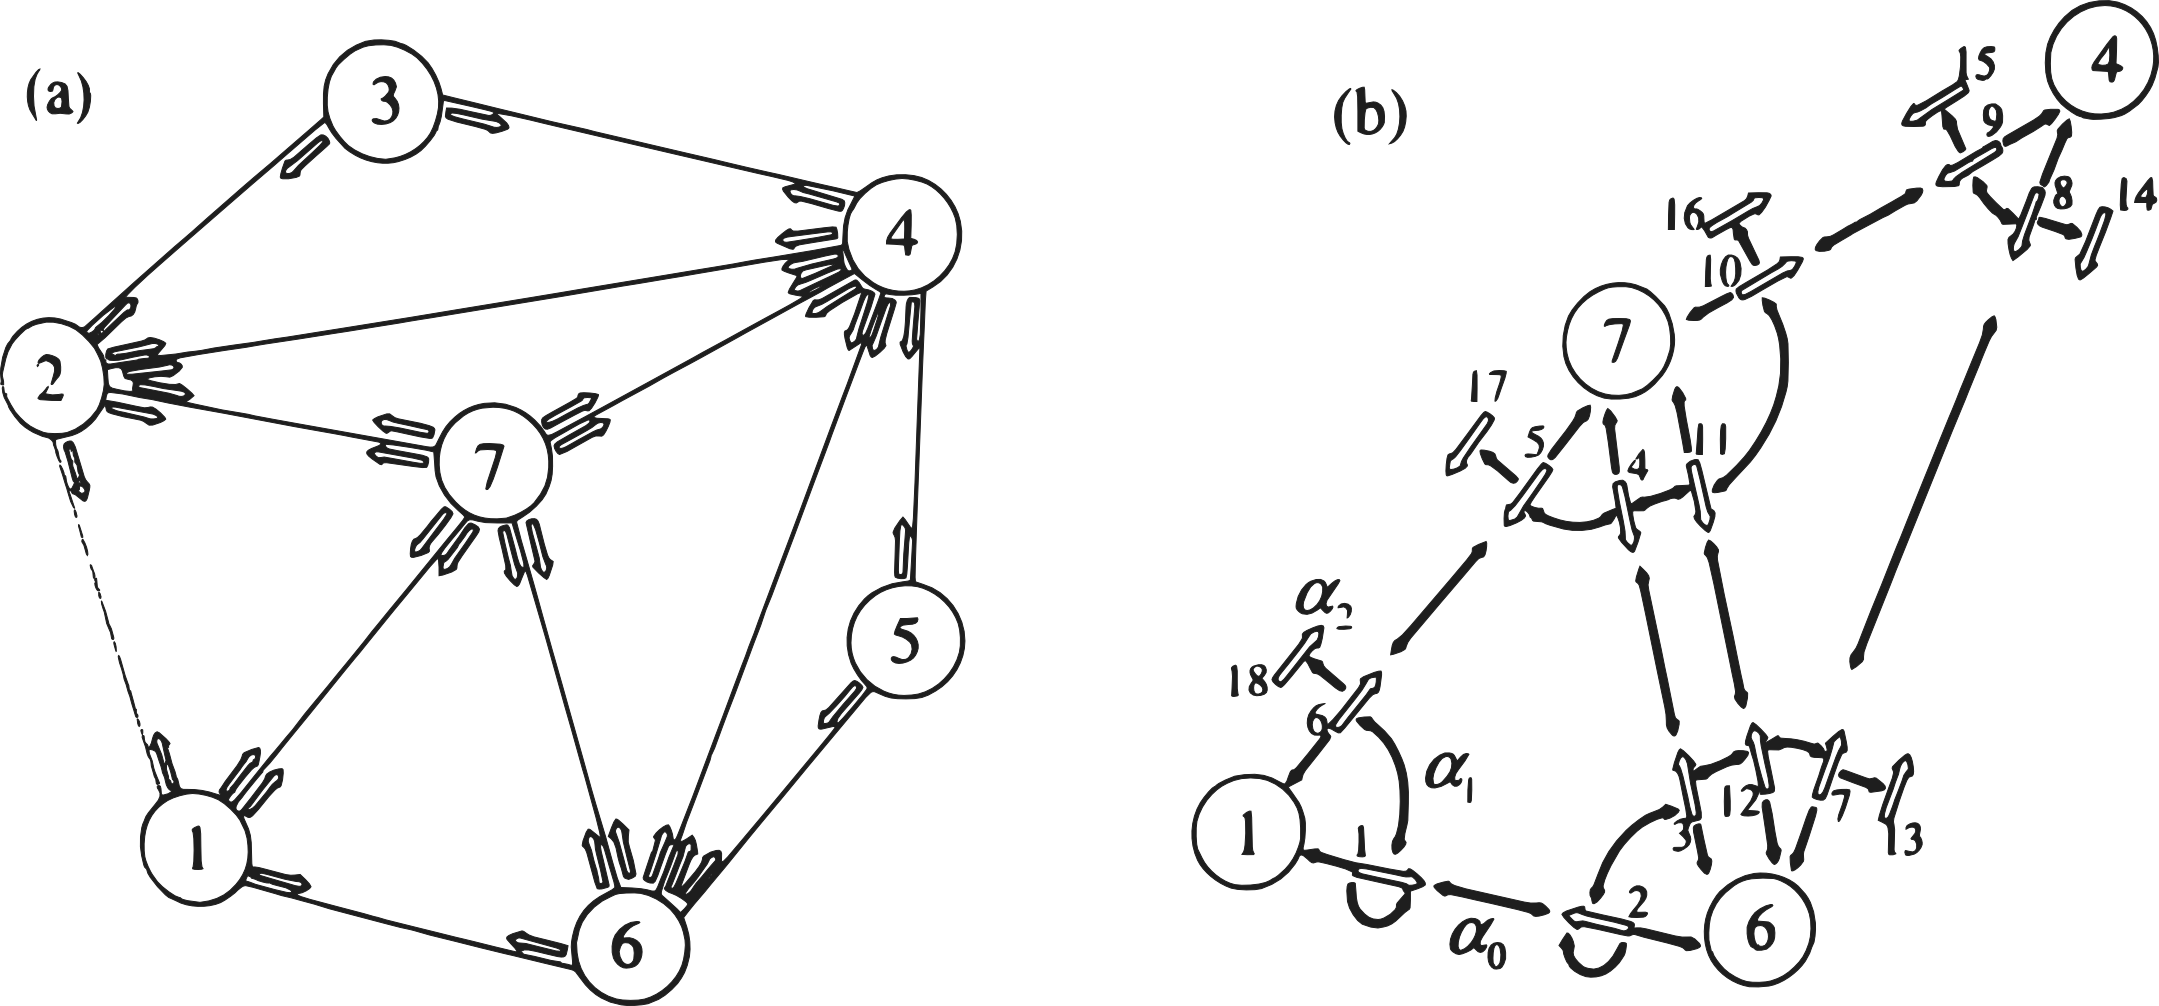
\includegraphics[width=0.8\textwidth]{img/dart_struct.png}
\caption{Dart-based datová struktura, zdroj: \cite{triangulation}}
\label{fig:dart_struct}
\end{figure}

\begin{table}[h!]
\catcode`\-=12
\begin{tabular}{|c||c|c|c|c|}
\hline
\multirow{2}{*}{Dart d} & \multicolumn{4}{c|}{Dartové pointery} \\ \cline{2-5} 
                         & Vrchol &$\alpha_0$ & $\alpha_1$ & $\alpha_2$      \\ \hline
1                        & 1          & 2      & 6      & 1      \\ \hline
2                        & 6          & 1      & 3      & 2      \\ \hline
3                        & 6          & 4      & 2      & 12     \\ \hline
4                        & 7          & 3      & 5      & 11     \\ \hline
5                        & 7          & 6      & 4      & 17     \\ \hline
6                        & 1          & 5      & 1      & 18     \\ \hline
7                        & 6          & 8      & 12     & 13     \\ \hline
8                        & 4          & 7      & 9      & 14     \\ \hline
9                        & 4          & 10     & 8      & 15     \\ \hline
10                       & 7          & 9      & 11     & 16     \\ \hline
11                       & 7          & 12     & 10     & 4      \\ \hline
12                       & 6          & 11     & 7      & 3      \\ \hline
\end{tabular}
\caption{Dart based struktura}
\label{tab:dart_based}
\end{table}

\newpage
\section{Interpolace metodou přirozeného souseda}

Interpolace metodou přirozeného souseda je deterministická
interpolační metoda pro prostorová data. Poskytuje spojitý, vyhlazený
výstup, bez extrapolovaných hodnot.

Pro výpočet vah využívá Voronoiových diagramů. Do VD pro měřené body
vkládá body určené k interpolaci. Vložením nového bodu dojde v jeho
okolí k přetvoření VD. K vypočtení váhy se používá jak VD před
vložením bodu, tak VD po vložení bodu. Voronoiova buňka nově vloženého
bodu překrývá několik buněk z~původního VD. Právě tento překryv, který
nově vložený bod \uv{ukradne} z plochy původních buněk slouží k
výpočtu váhy pro interpolaci.

\subsection{Lineární interpolace}
\label{sub:linear}
\bigskip
Matematicky tedy můžeme zapsat:
\newline
$$V(p)=\sum_{i=1}^n V_i$$

\noindent kde $V(p)$ je plocha nově vloženého bodu a $V_i$ je část
plochy původních buněk, o kterou byly vložením buňky \uv{okradeny}.

\bigskip
\noindent Váha pro jednotlivé sousedy se vypočte:
\newline
$$\lambda_i = \frac{V_i}{\sum_{i=1}^n V_i}$$

\bigskip
\noindent A konečně samotná hodnota pro interpolovaný bod není nic jiného než vážený průměr:
\newline
$$G(x,y) = \sum_{i=1}^{n} \lambda_i  f(x_i, y_i)$$

\newpage
\begin{figure}[h!]
\centering
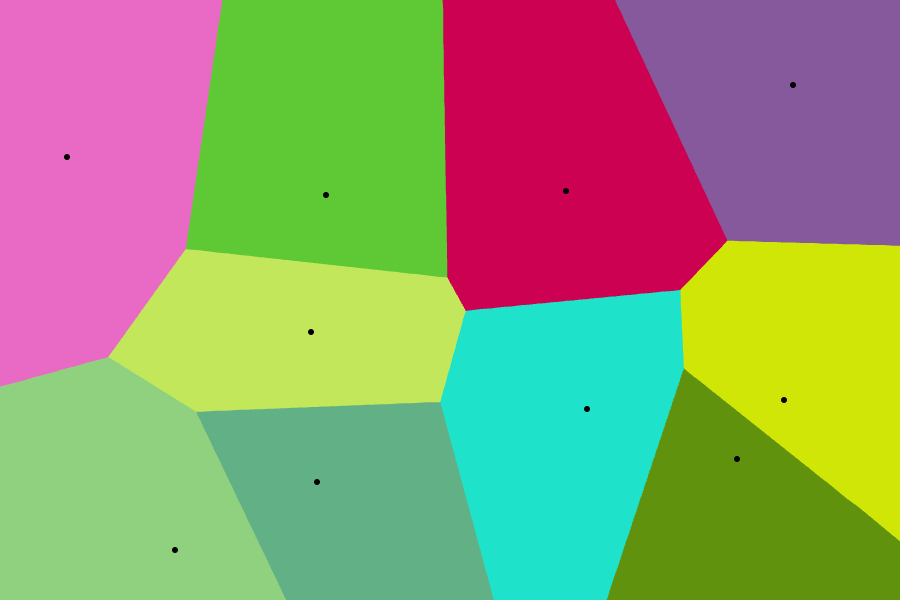
\includegraphics[width=0.7\textwidth]{img/canvas_0.png}
\caption{Původní VD}
\label{fig:fig:canvas0}
\end{figure}

\begin{figure}[h!]
\centering
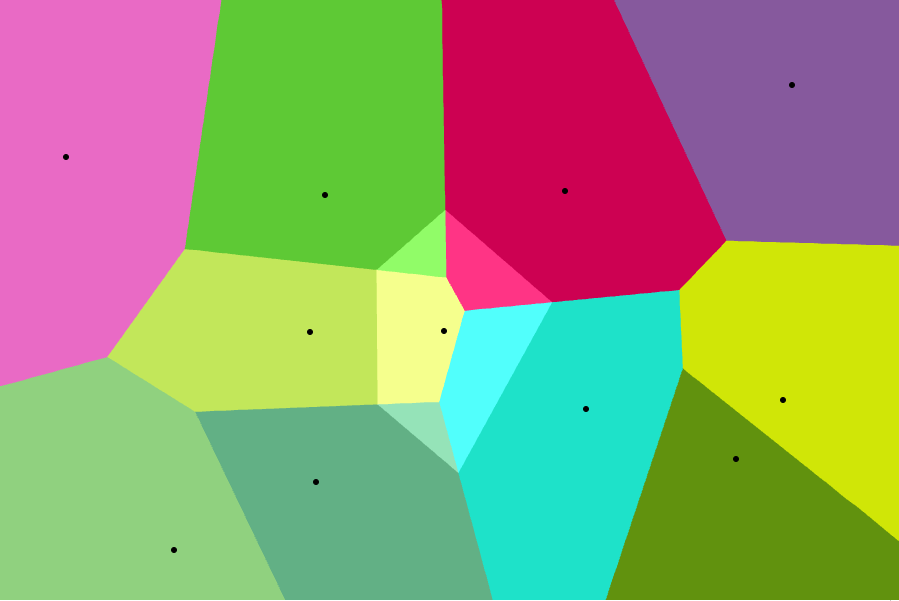
\includegraphics[width=0.7\textwidth]{img/canvas_1.png}
\caption{Ukradené plochy}
\label{fig:fig:canvas1}
\end{figure}

Na obrázku \ref{fig:fig:canvas1} vidíme, že nově vzniklá buňka \uv{ukradla} nejvíce plochy ze žlutého polygonu, nejméně ze zeleného. Při výpočtu funkční hodnoty vloženého bodu bude mít tedy hodnota žlutého polygonu největší váhu, zatímco hodnota zeleného bodu váhu nejmenší.\footnote{Vytvořeno pomocí \url{http://alexbeutel.com/webgl/voronoi.html}}
\begin{figure}[h!]
\centering
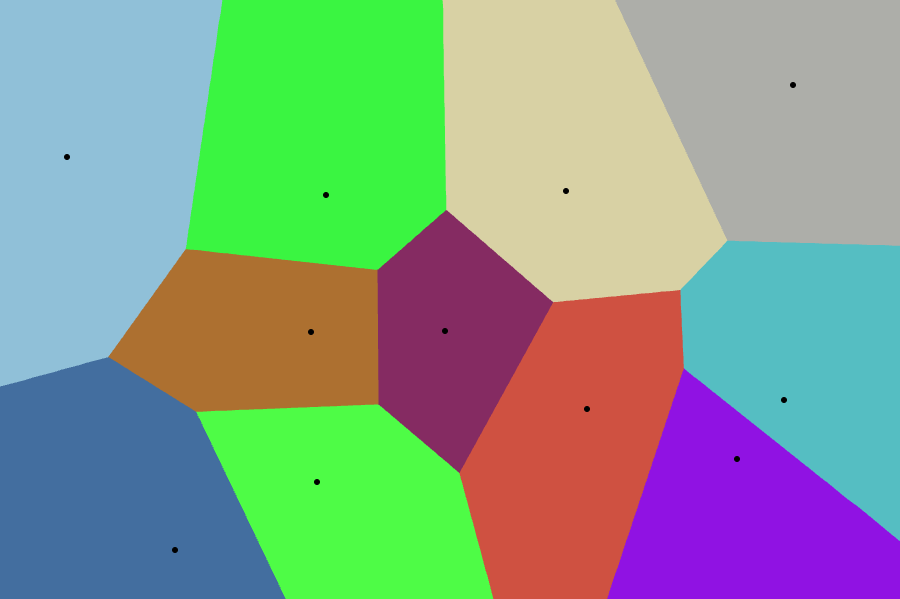
\includegraphics[width=0.7\textwidth]{img/canvas_2.png}
\caption{Nově vzniklý VD}
\label{fig:fig:canvas2}
\end{figure}

\newpage
\subsection{Sibsonova interpolace}
\label{sub:Sibson}
Sibsonova\footnote{Robin Sibson (narozen 1944), britský matematik. Jako první přišel s myšlenkou interpolace metodou přirozeného souseda.} interpolace je další metoda interpolace, která kromě vah přirozených sousedů počítá s funkcí gradientu $\nabla_i$ pro všechny $p_i \in P$. Metoda počítá gradient na základě vážených nejmenších čtverců roviny procházející sousedními body.Více o tomto tématu zde: \cite{Bobach} \cite{CGAL}.

\subsection{Farinova interpolace}
\label{sub:Farin}
%%% konzultace s Mayrem
%%% ML: jak to dopadlo?
%%% AL: ken konzultaci nedoslo, nasel jsem o tom nejake prameny na netu, moc tomu nerozumim,
%%% dal jsem sem jen par obecnych vet, ale nevim, zda tu nenechat jen tu linearni
Profesor Gerald Farin přišel s mnohem obecnějším přístupem, který není omezen na souřadnice přirozených sousedů, ale může použita pro všechny lokální souřadnice. Váha $\lambda$ může být vnímána jako barycentrická souřadnice v Bezierovu simplexu. Více zde: \cite{Bobach} \cite{CGAL}.

\newpage	
\part{Praktická část}

\newpage
\section{Postup řešení}
\subsection{Bash}
\label{sub:Bash}

Při řešení otázky, jak implementovat metodu přirozeného souseda pro
GRASS 7, se vycházelo z modulu napsaného pro GRASS GIS 6. Jednalo se o
modul \emph{v.surf.nnbathy} pro vektorová data. Tento modul byl napsán
%%% ML: to neni presne, spise se jedna po POSIX shell skript, skript
%%% muze bezet i v jinych interpretech, jako napr. csh ci zsh.
%%% AL: pouziti terminu shellovy skript
jako shellový skript. Pro novou verzi GRASS GISu 7, ve které si vývojáři kladou za
cíl zpřístupnit tento software širší veřejnosti, ovšem tento shellový skript nebylo možno použít, neboť do nové verze se počítá pouze s
moduly v jazyce Python a C/C++.

\subsubsection{v.surf.nnbathy}
%%% ML: viz poznamka k Bashi vyse
%%% AL: pouzit shellovy skript
\emph{v.surf.nnbathy}\footnote{\url{http://grass.osgeo.org/grass64/manuals/addons/v.surf.nnbathy.html}}
je shellový skript. Slouží jako interface mezi příkazem \emph{nnbathy} z
externí knihovny \emph{nn-c} a GRASS GISem. \emph{v.surf.nnbathy}
nabízí celkem tři algoritmy interpolace. Defaultně je nastaven
%%% ML: jsou nekde tyto metody rozepsany v teoreticke casti?
%%% AL: doplneno v teorii, pridany odkazy
\emph{Watson's algortithm for Sibson natural neighbor
  interpolation}, viz kapitola \ref{sub:Sibson}. Další možností je \emph{linear Delaunay
  interpolation}, kapitola \ref{sub:Sibson} a poslední \emph{Belikov and Semenov's algorithm for
  non-Sibsonian natural neighbor interpolation}. Pro Delaunayvou
triangulaci, která je základem pro všechny tři algoritmy, se využívá
knihovny \emph{Triangle} napsanou Jonathanem Richardem
Schewchukem. Parametry pro spuštění modulu jsou tyto (nepovinné v
hranatých závorkách):

%%% ML: formatovani nic moc, za uzavirajici zavorkou pro nepovinne
%%% paramatry je navic mezera, neslo by to udelat lepe?
%%% AL: formatovani pomoci tabulky
\bigskip
\begin{tabular}{ll}
\textbf{output}& Proměnná typu \emph{string}, název výstupní rastrové mapy.\\
\textbf{input}& Proměnná typu \emph{string}, název vstupní vektorové mapy.\\
\textbf{[file]}& Proměnná typu \emph{string}, název vstupního souboru.\\
\textbf{[column]}& Proměnná typu \emph{string}, název sloupce z atributové tabulky,\\
\textbf{}& jehož data budou použity pro interpolaci.\\
\textbf{[layer]}& Proměnná typu \emph{integer}, nastavení, zda se jedná od 2D nebo 3D vektorová data.\\
\textbf{[where]}& Proměnná typu \emph{string}, SQL where podmínka.\\
\textbf{[alg]}& Proměnná typu \emph{string}, název použitého algoritmu.\\
\end{tabular}

\newpage
Volání v příkazové řádce pak může vypadat například takto:
\begin{lstlisting}[caption={bash version}]
user@my_comp:~$ v.surf.nnbathy input=input_vector_map output=output_raster_map zcolumn=value alg=nn
\end{lstlisting}

\subsection{Python}
\label{sec:python}

Jako první krok pro implementaci interpolace přirozeného souseda pro
GRASS GIS 7 bylo potřeba stávající modul v Bashi přepsat do
podporovaného programovacího jazyka. Pro verzi 7 bylo možné přepsat
modul buďto do jazyka C/C++ nebo Python. Z důvodu nepříliš velké
zkušenosti s programováním byl pro začátek zvolen jazyk Python.
Nicméně ačkoliv byl modul přepsán do Pythonu, takže už mohl být 
použit i pro GRASS GIS 7, stále přetrvávala závislost na knihovně \emph{nn-c}.
%%% ML: tady bych jeste zminil, ze zavislost zustala stejne jako u
%%% shell skriptu, tj. nn-c. To je podstatna informace, ktera by tady
%%% mela byt zminena.
%%% AL: Doplněno

\subsubsection{v.surf.nnbathy.py}

V následující části této práce bude popsáno, jak Python modul
funguje, jaká jsou vstupní a výstupní data, jaké vytváří dočasné
soubory.

\paragraph{Vstupní data}

Stejně jako původní shellový skript, i tento modul pracuje se vstupními
daty buď v podobě textového ASCII souboru nebo vektorové mapy.

V případě použití vstupní vektorové mapy s body je pak při volání
modulu použit parametr \emph{column}, který určuje z jakého sloupce
atributové tabulky se budou brát hodnoty k interpolaci.

\begin{figure}[h!]
\centering
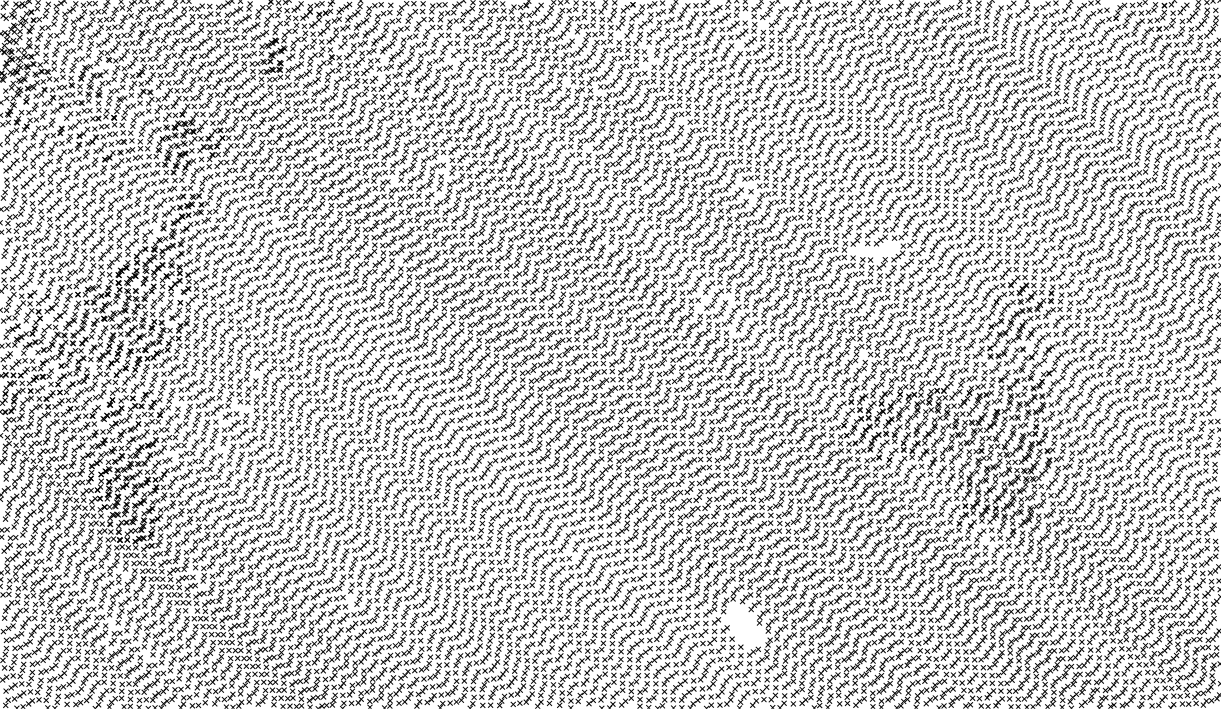
\includegraphics[width=0.9\textwidth]{img/vstup_vect_map.png}
\caption{Vektorová mapa na vstupu}
\label{fig:vstup_vect_map}
\end{figure}

\newpage

Druhou možností je použít textový ASCII soubor, který musí obsahovat
$n$ bodů na $n$ řádcích ve čtyřech sloupcích. V prvních dvou sloupcích
je uložen údaj o poloze v podobě x a y souřadnice. Ve třetím sloupci
jsou pak uloženy hodnoty veličiny, kterou chceme interpolovat a v
posledním sloupci nalezneme id bodu.

%ukazka TMPXYZ
\begin{lstlisting}[caption={Příklad vstupního souboru}]
639524.309 221227.596 112.191 101960
639529.088 221223.045 112.225 101961
639529.152 221219.826 112.029 102115
639524.303 221224.435 112.212 102116
639519.444 221229.043 111.752 102117
639513.546 221229.699 111.472 102440
639518.307 221225.172 111.874 102441
639523.114 221220.597 112.243 102442
\end{lstlisting}

\bigskip
\paragraph{Funkce region()}

Každá operace prováděná v GRASS GISu je prováděna pouze na určitém
rozsahu území, tzv. \emph{výpočetním regionu}. \emph{Výpočetní region}
%%% ML: kartograficke souradnice jsou zavadejici, pripadne pouzij zemepisne souradnice
%%% AL: opraveno
je určen jako obdélník daný mezními zeměpisnými souřadnicemi a
počtem řádků a sloupců.  Funkce \emph{region()} všechna nastavení
uloží do proměných. Dále vypočte plochu výpočetního regionu. Na rozdíl
od GRASS GISu, který jako mezní kartografické souřadnice bere vnější
rohy rohových buněk obdélníku, knihovna \emph{nn-c} používá středy
rohových buněk, a proto je třeba nastavení výpočetního regionu opravit
o rozlišení buněk.

\bigskip
\paragraph{Funkce initials\_controls()}

Ve chvíli, kdy je nastavený výpočetní region, můžeme provést úvodní
kontroly a přípravy před samotným výpočtem. Zejména zda plocha
výpočetního regionu není nulová a je kde provádět interpolaci. Dále je
třeba zajistit jednoznačné určení vstupních dat, tedy zda se bude
pracovat s ASCII souborem, nebo vektorovou mapou, a jejich kontrolu,
popřípadě SQL podmínku. Také kontrolujeme, zda z knihovny \emph{nn-c}
máme nainstalovaný program \emph{nnbathy}, který interpolaci
provádí. Též je třeba vytvořit dočasné pomocné soubory, které
využijeme při práci s daty.

V případě, že pracujeme s vektorovou mapu, uložíme informace o
bodových datech do dočasného proměnné \emph{TMPcat} pomocí modulu
\emph{v.out.ascii}. Výstupem toho modulu je ASCII soubor o $n$ řádcích
a čtyřech sloupcích. V prvních dvou sloupcích je uložená poloha bodu,
ve třetím jeho id a ve čtvrtém hodnota k interpolaci.

\bigskip
%ukazka souboru TMPcat
\lstset{basicstyle=\footnotesize}
\begin{lstlisting}[caption={Pomocný soubor TMPcat}]
638234.122902785427868 221198.4894384436775   1 62.817782000000001
638755.665974545176141 220976.783764891704777 2 9.190488000000000
638729.530741120455787 219988.669646041787928 3 91.799952000000005
638088.941303733270615 220228.186909802345326 4 76.839046999999994
638158.578729554312304 220794.514421981060877 5 2.037001000000000
637781.724264170858078 219988.193243810994318 6 8.298977000000001
638359.847223712014966 220692.375897407706361 7 15.550326000000000
639137.670258715632372 221096.622500944242347 8 16.613054999999999
\end{lstlisting}

Jelikož id bodu k dalším výpočtům nepotřebujeme do dočasné proměnné
\emph{TMPXYZ} si uložíme pouze informace o poloze a hodnotu k
interpolaci. V případě, že nepracujeme s vektorovou mapou, ale ASCII
souborem, tak tento soubor rovnou uložíme do proměnné \emph{TMPXYZ}.

\bigskip
%ukazka souboru TMPxyz
\lstset{basicstyle=\footnotesize}
\begin{lstlisting}[caption={Pomocný soubor TMPXYZ}]
638234.122902785427868 221198.489438443677543 62.817782000000001
638755.665974545176141 220976.783764891704777 9.190488000000000
638729.530741120455787 219988.669646041787928 91.799952000000005
638088.941303733270615 220228.186909802345326 76.839046999999994
638158.578729554312304 220794.514421981060877 2.037001000000000
637781.724264170858078 219988.193243810994318 8.298977000000001
638359.847223712014966 220692.375897407706361 15.550326000000000
639137.670258715632372 221096.622500944242347 16.613054999999999
\end{lstlisting}

\bigskip
\paragraph{Funkce compute()}

V této části kódu je volán program \emph{nnbathy} s následujícími
vstupními paramatry:
\begin{description}
\item[-w]{proměnná typu \emph{double}, omezuje extrapolaci přiřezením minimální váhy pro vrchol Delaunayovi sítě. Defaultně je nastavena nula, což zamezuje extrapolaci.}
\item[-i]{proměnná typu \emph{string}, název vstupního souboru o $n$ řádcích, se třemi sloupci, x a y souřadnicí a hodnotou k interpolaci}
\item[-x]{dvojice $x_{min}$, $x_{max}$ typu \emph{double}, mezní hodnoty výstupní mřížky}
\item[-y]{dvojice $y_{min}$, $y_{max}$ typu \emph{double}, mezní hodnoty výstupní mřížky}
\item[-P]{proměnná typu \emph{string}, použitá metoda interpolace}
\item[-n]{dvojice \emph{double} x \emph{double}, rozlišení výstupní mřížky}
\end{description}

Výstupem z \emph{nnbathy} je soubor \emph{XYZout}. Obsahuje data o
výstupní mřížce buňku po buňce ve třech sloupcích. V prvních dvou jsou
x a y souřadnice, ve třetím vyinterpolovaná hodnota. V případě buňek
mimo oblast, kde probíhala interpolace, je ve třetím sloupci uložena
hodnota NaN.

\bigskip
%ukazka XYZout
\lstset{basicstyle=\footnotesize}
\begin{lstlisting}[caption={XYZout}]
637725 221045 NaN
637735 221045 NaN
637745 221045 NaN
637755 221045 NaN
637765 221045 NaN
637775 221045 23.2274425578696
637785 221045 20.3234644594092
637795 221045 23.6841650075168
\end{lstlisting}

\bigskip
\paragraph{Funkce convert()}

Výstupní textový soubor z \emph{nnbathy} je třeba upravit, aby s ním
bylo možné dále pracovat v GRASS GISu. Pro další práci slouží dočasný
soubor \emph{TMP}. Při vytváření na začátku tohoto souboru vznikne
hlavička, která obsahuje data o hraničních souřadnicích, prostorovém
rozlišení, datovém typu a hodnotě žádná data (null či NaN).

\newpage
%Ukázka hlavičky
\lstset{basicstyle=\ttfamily}
\begin{lstlisting}[caption={Hlavička souboru TMP}]
north: 228495.0
south: 215005.0
east: 644995.0
west: 630005.0
rows: 1350
cols: 1500
type: double
null: NaN
\end{lstlisting}

Dále je potřeba vybrat vyinterpolované hodnoty jednotlivých buněk ze
souboru \emph{XYZout}, kde jsou uloženy ve třetím sloupci na
samostatných řádcích, a vložit je do souboru \emph{TMP} v pravidelné
mřížce.

%ukázka souboru TMP
\lstset{basicstyle=\footnotesize}
\begin{lstlisting}
NaN NaN NaN NaN NaN NaN NaN  20.7543487721 21.6412738464 21.0697741691 
NaN NaN NaN NaN 22.0420316367 21.2339890563 22.1237145752 20.8684520153 
NaN NaN NaN 21.1184005087 21.2163721800 22.5528243734 20.6780204446 
NaN NaN NaN NaN 20.1954939692 22.8280745872 21.2507738978 21.6682239762 
NaN NaN NaN 20.8488929136 21.3643657768 21.6917150115 20.9860960516 
NaN NaN 20.3606443297 21.3323845603 22.8051229299 21.8176089189 
NaN NaN 20.3078295678 20.6627164743 21.8458254363 21.2712885642 
21.6370709432 21.1827185754 21.6464451799 21.2912057725 NaN NaN NaN NaN 
22.6809840563 21.6959007615 20.1153796499 20.1067779317 NaN NaN NaN NaN 
22.3064205177 20.8191889879 20.8209937444 22.1952518030 NaN NaN NaN NaN 
NaN NaN NaN NaN NaN NaN NaN NaN NaN NaN NaN NaN NaN NaN NaN NaN NaN NaN 

\end{lstlisting}

\newpage
\paragraph{Funkce import\_to\_raster()}

Soubor \emph{TMP}, ve kterém máme uložené vyinterpolované hodnoty v
pravidelné mřížce, slouží jako vstupní soubor pro GRASS modul
\emph{r.in.ascii}, který tyto hodnoty převedu do rastru. Dále je
použit modul \emph{r.support}, který uloží příkazy do rastrových
metadat. Na závěr je vytištěna zpráva, že byla vytvořena rastrová
mapa.

\paragraph{Výstupní data}
Výstupem modulu \emph{v.surf.nnbathy} je rastrová mapa.

%%% ML: dal bych jsem alespon legendu
\begin{figure}[h!]
\centering
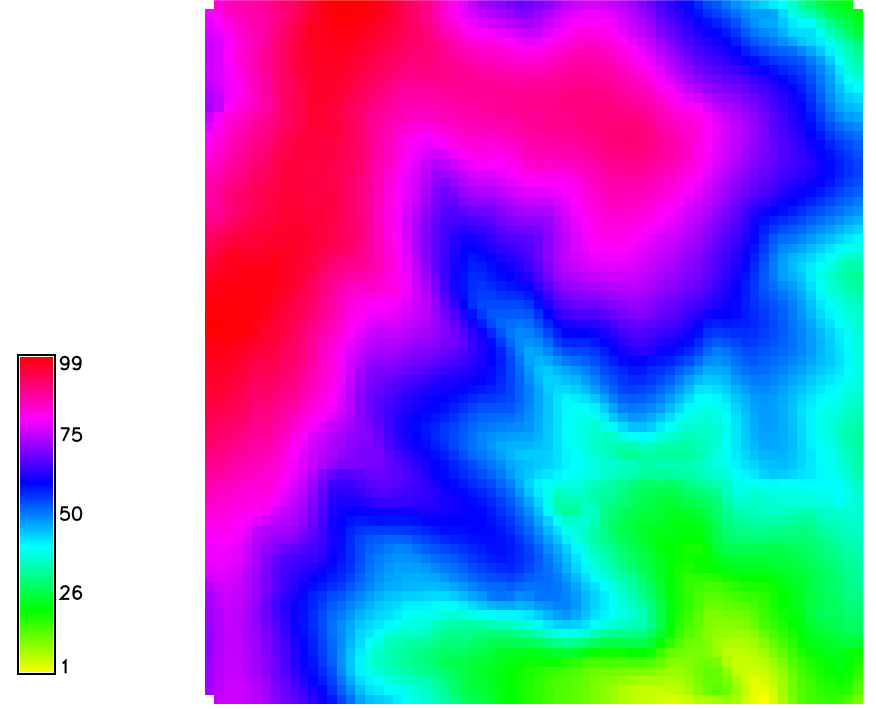
\includegraphics[width=0.9\textwidth]{img/vystup_rast_map.png}
\caption{Výstupní rastrová mapa}
\label{fig:vystup_rast_map}
\end{figure}

\newpage
\subsection{OOP- Objektově orientované moduly}
%%% ML: mozna bych tu zkratku v nazvu rezepsal
%%% AL: rozepsano

V průběhu práce na Python modulu \emph{v.surf.nnbathy} bylo
%%% ML: v textu bych nahradil Bash skript za shellový skript
%%% AL: nahrazeno
zjištěno, že v GRASS GISu verze 6 je k dispozici také shellový skript
\emph{r.surf.nnbathy}, který pracuje s rastrovými daty. Jelikož větší
část kódu byla pro moduly \emph{v.surf.nnbathy} a \emph{r.surf.nnbathy} společná,
byla hlavní výpočetní část spojena. Na místo dvou procedurálních
modulů byla objektově vytvořena knihovna \emph{nnbathy.py} (příloha \ref{app:nnbathy}) a dva
moduly \emph{v.surf.nnabthy.py} (příloha \ref{app:v.surf}) pro vektorová data a
\emph{r.surf.nnbathy.py} (příloha \ref{app:r.surf}) pro data rastrová, které knihovnu
\emph{nnbathy} volají.

\subsubsection{v.surf.nnbathy}

%%% ML: prilis dlouha veta
%%% AL: zkraceno
Z nového objektově orientovaného modulu pro vektorová data \emph{v.surf.nnbathy} tak zmizela výpočetní část kódu. Zůstala úvodní část, která automaticky generuje GUI,
úvodní vstupní kontroly a dále podmínka, která vyhodnocovala, zda vstupují data v podobě
vektorové mapy nebo ASCII souboru.

\subsubsection{r.surf.nnbathy}

Modul \emph{r.surf.nnbathy} pracuje na podobném principu jako modul
\emph{v.surf.nnbathy}, jen pro rastrová data. Při volání je možnost
použít méně parametrů.

\begin{tabular}{ll}
\textbf{output}& Proměnná typu \emph{string}, název výstupní rastrové mapy.\\
\textbf{input}& Proměnná typu \emph{string}, název vstupní vektorové mapy.\\
\textbf{[alg]}& Proměnná typu \emph{string}, název použitého algoritmu.\\
\end{tabular}

I v tomto modulu zůstala část, která vytváří GUI. Protože ale modul
pracuje s daty pouze v podobě rastrové mapy, nebyly potřeba žádně
vstupní kontroly.

\newpage
\subsubsection{nnbathy}

V knihovně {\em nnbathy}, (příloha \ref{app:nnbathy}) kterou oba moduly volají, tedy zůstala hlavní
výpočetní část kódu.

\paragraph{Rodičovská třída Nnbathy} V rodičovské třídě Nnbathy bylo
vytvořeno několik objektů, které přebraly funkce jednotlivých procedur

%%% To nejsou objekty, ale metody, resp. konstruktor a desktruktor
%%% AL: opraveno
z předchozího kódu. Navíc byly vytvořeny tyto metody:

\paragraph{Metoda \_\_init\_\_}
%%% ML: objekt -> metoda
%%% AL: opraveno
Tato metoda- konstruktor inicializuje dočasné soubory a volá objekt region().

\paragraph{Metoda \_\_del\_\_}
Tato metoda- destruktor slouží k odstranění dočasných souborů.

\paragraph{Třída Nnbathy\_raster}
%%% ML: je dedicka z - nezni moc cesky...
%%% AL: opraveno na dedicka
Tato třída slouží pro rastrová vstupní data a je dědická z rodičovské třídy Nnbathy.

\paragraph{Třída Nnbathy\_vector}
Tato třída slouží pro vektorová vstupní data a je dědická z rodičovské třídy Nnbathy.

\paragraph{Třída Nnbathy\_file}
Tato třída slouží pro vstupní data v podobě ASCII souboru a je dědická z rodičovské třídy Nnbathy.

\todo[inline]{MLU diagram}

\newpage
\section{Možnosti budoucí implementace}
V současné době jsou oba moduly k dispozici v rámci balíčků
Add-Ons\footnote{http://grass.osgeo.org/download/addons/}. V adresáři
\emph{grass7/vector/v.surf.nnbathy} můžeme naleznout hlavní knihovnu
\emph{nnbathy.py}, modul \emph{v.surf.nnbathy.py} a dokumentaci
\emph{v.surf.nnbathy.html}.

V adresáři \emph{grass7/raster/r.surf.nnbathy} naopak nalezneme modul
\emph{r.surf.nnbathy.py} a jeho dokumentaci
\emph{v.surf.nnbathy.html}. Oba moduly je možné instalovat do GRASS
GISu 7, pomocí modulu \emph{g.extention} nebo pomocí GUI.

\bigskip
\begin{lstlisting}[caption={Stáhnutí modulu v.surf.nnbathy pomocí g.extention}]
g.extension extension=v.surf.nnbathy
\end{lstlisting}

\bigskip 

%%% ML: ta prvni veta zni divne
V současné chvíli tedy tyto moduly nejsou součástí oficiální distribuce GRASS GISu, 
ale pouze v rámci Add-Ons. Jelikož interpolace metodou přirozeného souseda poskytuje
spojité, hladké výstupy bez extrapolovaných hodnot může být její
použití v praxi poměrně využívané. Právě proto je snaha dostat tento
interpolační nástroj do základní distribuce GRASS GISu. Tomu však
brání vnitřní závislost na knihovně \emph{Triangle}, která nespadá pod volně
šiřitelnou licenci GNU GPL. V následujících kapitolách rozebereme
možnosti vyhnutí se této knihovně a následné implementace.

\newpage
\subsection{Knihovna Triangle}

Knihovna Triangle verze
1.4\footnote{\url{http://www.cs.cmu.edu/~quake/triangle.html}} byla napsaná
Jonathanem Richardem Shewchuk v roce 2002. Bohužel není distribuována pod
%%% ML: kde jsi tohle nasel???
%%% ML: citace ze stranek "Please note that although Triangle is
%%% freely available, it is copyrighted by the author and may not be
%%% sold or included in commercial products without a license."""
%%% AL: opraveno
volně šiřitelnou licencí která by dovolila její začlenění do oficiální distribuce GRASS
GISu. V programu \emph{nnbathy} má na starosti Delaunayovu
triangulaci. Je tedy třeba najít vhodný způsob, jak tuto knihovnu
nahradit.

Triangle pro tvorbu triangulace využívá Divide and Conquer algoritmus,
viz kapitola \ref{subsec:DnC_alg}, v kombinaci s Inkrementálním
algoritmem, kapitola \ref{subsec:Inc_alg}. Pro ukládání dat využívá
svoji vlastní, poměrně obsáhlou datovou strukturu \emph{delaunay}
(Příloha \ref{app:delaunay_struct}), do které si ukládá hraniční body
regionu, všechny body triangulace, všechny trojúhelníky s hranami a
jejich opsanými kružnicemi, včetně jejich sousedů.

Tuto datovou strukturu \emph{delaunay} dále využívá i samotný program
\emph{nnbathy}, který provádí interpolaci metodou přirozeného
souseda. Právě převod na tuto datovou strukturu bude v budoucnosti
klíčový v případě, že se podaří najít vhodný triangulační nástroj,
který nahradí knihovnu Triangle.

\newpage
\subsection{Modul \emph{v.delaunay}}
\label{subsec:v.delaunay}

Modul
\emph{v.delaunay}\footnote{\url{http://grass.osgeo.org/grass70/manuals/v.delaunay.html}}
je součástí oficiální distribuce GRASS GISu. Tento modul poskytuje
Delaunayovu triangulaci nad vektorovou mapou s body nebo
centroidy. Pro vytvoření triangulace používá modul algoritmus Rozděl a
panuj, viz kapitola \ref{subsec:DnC_alg}. Data ukládá do datové
struktury winged-edge, kapitola \ref{subsec:HE_struct}, též příloha \ref{app:edge_struct}.

\begin{figure}[h!]
\centering
\begin{floatrow}
\ffigbox{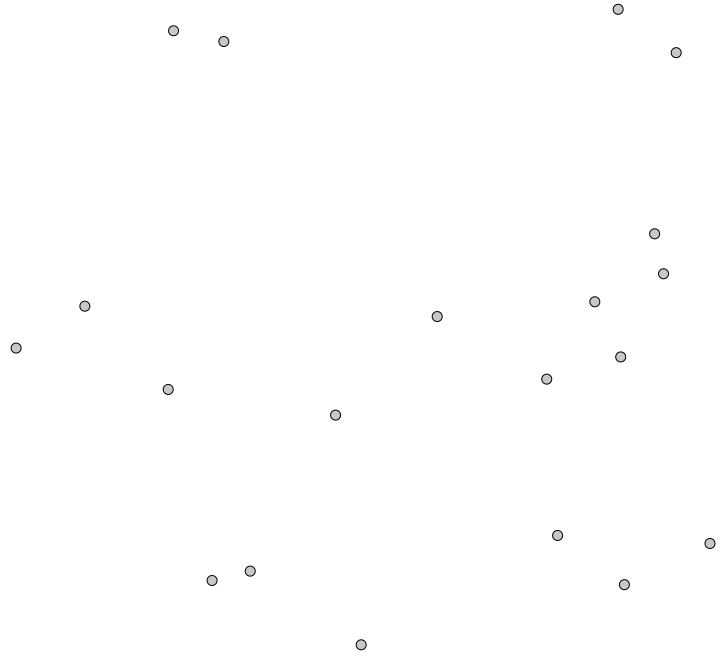
\includegraphics[width=0.48\textwidth]{img/b20.png}}{\caption{Množina bodů pro triangulaci}}{\label{fig:b20}}
\ffigbox{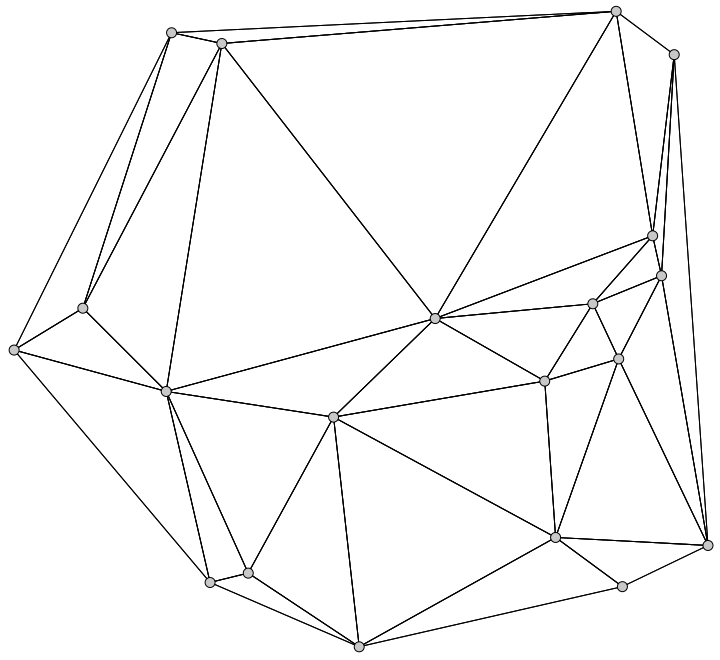
\includegraphics[width=0.48\textwidth]{img/b20_del.png}}{\caption{Triangulace pomocí v.delaunay}}{\label{fig:b20_del}}
\end{floatrow}
\end{figure}

Ovládání modulu je velmi jednoduché na výběr máme pouze z několika
%%% ML: flag prekladej jako prepinac
%%% AL: přeloženo
přepínačů a několika paramatrů:

%%% ML: je to tady podstatne vubec uvadet???
%%% AL: dohodli jsme se, ze to tak nechame
\noindent Přepínače:
\begin{tabular}{ll}
\textbf{-r}& Počítej pouze s body v aktuálním regionu.\\
\textbf{-l}& Vytvoř výstupní triangulaci pomocí linií, ne ploch.\\
\end{tabular}

\noindent Parametry:
\begin{tabular}{ll}
\textbf{input}& Povinný parametr. Název vstupní vektorové mapy.\\
\textbf{[layer]}& Název nebo číslo vrstvy. Slouží k připojení do databáze.\\
\textbf{output}&  Povinný parametr. Název výstupní vektorové mapy.\\
\end{tabular}

%%% ML: chtelo by najit zpusob jako lokalizovat do cestiny Listings
\begin{lstlisting}[caption={Volání modulu v.delaunay z příkazové řádky}]
v.delaunay input=input_map output=output_map
\end{lstlisting}

\bigskip
\subsection{Převod mezi strukturami}

Z hlediska rychlosti se modul \emph{v.delaunay} jeví jako adekvátní
náhrada za knihovnu Triangle. Při testech bylo dokázáno, že pro
náhodné konfigurace miliónu bodů dokáže triangulaci provést za méně
než 15 s, což se dá považovat za dostatečně efektivní. 

Jako problémová se jeví část převodu dat mezi
strukturami. \emph{v.delaunay} používá strukturu edge (příloha \ref{app:edge_struct}),
což je běžná datová struktura typu winged-edge, viz kapitola \ref{subsec:HE_struct}. Naproti tomu \emph{Nnbathy} počítá interpolaci nad daty uloženými ve
%%% ML: uvadis nekde strukturu, kterou pouziva GRASS modul?
%%% AL: struktura winged-edge pridana do priloh
struktuře \emph{delaunay} (Příloha \ref{app:delaunay_struct}), která
je poměrně netypická, protože data ukládá do polí za pomocí pointerů a
indexů zároveň.

Nicméně naplnění struktury \emph{delaunay} možné je, byť vyžaduje
několikerý průchod přes všechny hrany triangulace. Na jeden průchod je
možné získat celkový počet bodů \emph{n}, získat \emph{id}
jednotlivých trojúhelníků, \emph{id} jejich vrcholů a vypočítat středy
opsaných kružnic. Dále je nutné označit pro každý trojúhelník jeho
sousedy, tedy trojúhelníky, který s ním sdílí hranu. Opět je třeba
projít celou triangulaci. Během tohoto průchodu je pravděpodobné, že
se dostaneme k již zpracovanému trojúhelníku. Proto bude třeba
vytvořit např. pomocný vektor typu boolean, do kterého se bude
ukládat, zda trojúhelník už byl zpracován či nikoliv. Nejsložitější je
naplnění struktur \emph{n\_point\_triangles} a \emph{point\_triangles}
(viz Příloha \ref{app:delaunay_struct}). Zde je ke každému bodu
přiřazen počet trojúhelníků, do kterých náleží a jejich
\emph{id}. Opět je zapotřebí několikerý průchod strukturou winged-edge
a pomocná struktura, do které budeme ukládat seznam \emph{previous
  edge}.

Po delším zkoumání tedy bylo zjištěno, že převod mezi strukturami
možný je. Nicméně časová i výpočetní náročnost společně s faktem, že
se jedná o dost \uv{kostrbaté} řešení, ukázaly, že samotná náhrada
knihovny \emph{Triangle} jiným nástrojem, který bude zajišťovat DT,
není správnou cestou. Největším problémem tohoto řešení je, že
\emph{Nnbathy} využívá strukturu \emph{delaunay}, která je poměrně
netypická, takže je hůře kompatibilní s jakýmikoliv jinými
triangulačními nástroji, které používají běžné datové struktury.

Pro další řešení se tedy hledal takový nástroj, který by se nestaral
pouze o DT ale i o samotnou interpolaci. Tak by se bylo možné vyhnout
závislosti nejen na triangulačním nástroji, ale i na knihovně
\emph{nn-c}.

\newpage
\subsection{Knihovna CGAL}

\todo[inline]{Dopsat na základě toho, co se zjistí.} 

Knihovna CGAL (The Computational Geometry Algorithms
Library)\footnote{\url{http://www.cgal.org}} je open source projekt, který
poskytuje snadný přístup k efektivním a spolehlivým geometrickým
algoritmům ve formě C++ knihovny. CGAL se používá v různých oblastech,
které potřebují geometrické výpočty, jako např. v GISech, CADu,
molekulární biologii, počítačové grafice a robotice. Knihovna CGAL je
distribuována pod licencí GNU GPL, což perfektně vyhovuje pro jeho
použítí pro GRASS GIS.

Jeden z balíčků této knihovny se přímo zabývá interpolací obecně ve 2D
i 3D, implementací funkcí na výpočet souřadnic přirozeného souseda a
různými metodami interpolace pro roztroušená prostorová data, z nichž
většina je založena právě na metodě přirozeného souseda. K dispozici
jsou celkem 4 interpolační metody a sice tyto:
\begin{itemize}
\item Linear Precision Interpolation (kapitola \ref{sub:linear})
\item Sibson's Continuous Interpolant (kapitola \ref{sub:Sibson})
\item Farin's Continuous Interpolant (kapitola \ref{sub:Farin})
\item Quadratic Precision Interpolants
\end{itemize}

\subsubsection{v.surf.nn}
\label{subsub:v.surf.nn}
V současné chvíli probíhá vývoj nového modulu \emph{v.surf.nn}, který
zatím využívá pouze metodu \emph{Linear Precision Interpolation}, tedy
pouze lineární interpolaci bez ohledu na gradient. Do budoucna se však
uvažuje o přidání i ostatních metod a možnosti nechat uživateli volbu,
kterou metodu chce použít.

\newpage
\section{Závěr}

Cílem této bakalářské práce byla implementace nástroje pro interpolaci
metodou přirozeného souseda do GRASS GISu. Jako první krok byly tedy v
Pythonu napsány dva moduly \emph{v.surf.nnbathy} pro vektorová data a
\emph{r.surf.nnbathy} pro rastrová data. Tyto moduly jsou v
současnosti k dispozici v GRASS GISu v rámci balíčků Add-Ons a
uživatel může po instalaci těchto rozšíření bez problému využívat
interpolaci metodou přirozeného souseda. Nicméně tyto moduly jsou
stále závislé na knihovně \emph{nn-c}, která provádí samotnou
interpolaci a hlavně na knihovně \emph{Triangle}, která se stará o
provedení DT a která je pod licencí MIT.

Dále se tato práce zabývala možností využít modulu \emph{v.delaunay},
který je už v~oficiální distribuci GRASS GISu, jako náhradu za
knihovnu \emph{Triangle}. V rámci zjišťování, zda je možné modul
\emph{v.delaunay} použít, byly detailně prostudovány jednotlivé
algoritmy, jak DT provést. Dále byly podrobně zkoumány datové
struktury, které se pro ukládání triangulací běžně využívají. Všechny
tyto poznatky byly zpracovány v~teoretické části v kapitolách
\ref{sec:algoritmy} a \ref{sec:data_struct}. Nicméně se ukázalo, že
ačkoliv náhrada knihovny \emph{Triangle} za modul \emph{v.delaunay} je
možná, tak převod mezi jednotlivými strukturami je příliš náročný a
neefektivní, zejména kvůli netypické struktuře \emph{delaunay}, kterou
knihovna \emph{nn-c} využívá.

Jako vhodné řešení se tedy ukázalo použití knihovny \emph{CGAL}. Tato
knihovna dokáže nejen vytvořit Delaunayho triangulaci, ale nabízí i
několik metod pro interpolaci metodou přirozeného souseda. Díky
použítí knihovny \emph{CGAL} dojde k zbavení se závislosti na
knihovnách \emph{nn-c} a \emph{Triangle}. Vývoj samotného modulu
\emph{v.surf.nn} a jeho implementace je aktuálně v procesu.

V rámci této bakalářské práce bylo též provedeno porovnání výkonu a
výstupu mezi GRASS GISem, zástupcem open source softwaru, a Esri ArcGIS,
proprietárním softwarem. Za GRASS GIS byl testován modul
\emph{v.surf.nnbathy} se závislostí na knihovně \emph{nn-c} a dále
modul \emph{v.surf.nn}, který je postavený na knihovně \emph{CGAL}. Za
Esri ArcGIS byl testován nástroj \emph{Natural Neighbour}, který se nachází
v toolboxu Spatial Analyst. Výsledky jsou uvedeny v Příloze
\ref{app:srovnani}



\newpage
\necislovana{Seznam použitých zkratek}

\begin{tabular}{ll}
\textbf{CGAL}& The Computational Geometry Algorithms Library\\
\textbf{DMT}& Digitální model terénu\\
\textbf{DT}& Delaunayova triangulace\\
\textbf{DPZ}& Dálkový průzkum Země\\
\textbf{GIS}& Geographic Information System (Geografický informační systém)\\
\textbf{GNU GPL}& GNU General Public License\\
\textbf{GRASS}& Geographical Resources Analysis Support System\\
\textbf{HW}& Hardware\\
\textbf{OS}& Operační systém\\
\textbf{QGIS}& Quantum GIS\\
\textbf{GUI}& Graphical User Interface (Grafické uživatelské rozhraní)\\
\textbf{USA-CERL}& US Army Construction Engineering Research Laboratories\\
\textbf{VD}& Voronoiův diagram\\
\end{tabular}

\newpage
\renewcommand\baselinestretch{1.2}
\selectfont
\renewcommand{\refname}{Použité zdroje}
\phantomsection
\addcontentsline{toc}{section}{\refname}


%%% ML: nenajdes jeste neco dalsiho co bys do literatury mohl pridat,
%%% deset kousku je dost malo
%%% AL: neco jsem pridal

\begin{thebibliography}{99}
\label{literatura}


\bibitem{triangulation}
HJELLE, Øyvind; DÆHLEN, Morten. \textit{Triangulations and applications}. Berlin: Springer, 2010. 234 s. ISBN 978-3-642-06988-8.


\bibitem{grafika}
SOCHOR, Jiří; ŽÁRA, Jiří. \textit{Algoritmy počítačové grafiky}. Praha: České vysoké učení technické, 1994. 258 s. ISBN 978-8-001-00949-9.


\bibitem{script}
GRASS Development Team. \textit{GRASS 7 Programmer's Manual} [online].
URL: \textless\url{http://grass.osgeo.org/programming7}\textgreater


\bibitem{trac}
\textit{GRASS GIS Tracker and Wiki} [online]. 
URL: \textless\url{http://trac.osgeo.org/grass}\textgreater


\bibitem{rukovet}
NETELER, Markus. \textit{Praktická rukověť ke geografickému informačnímu systému GRASS} [online].
URL: \textless\url{http://geo.fsv.cvut.cz/data/grasswikicz/grass_prirucka/grass_prirucka_0.4.pdf}
\textgreater

\bibitem{TB1}
BAYER, Tomáš. \textit{Rovinné triangulace a jejich využití} [online].
URL: \textless\url{https://web.natur.cuni.cz/~bayertom/Adk/adk5.pdf}
\textgreater

\bibitem{TB2}
BAYER, Tomáš. \textit{Voronoi diagram} [online].
URL: \textless\url{https://web.natur.cuni.cz/~bayertom/Adk/adk5.pdf}
\textgreater

\bibitem{Kohout}
KOHOUT, Josef. \textit{Paralelní Delaunayova triangulace
ve 2D a 3D} [online].
URL: \textless\url{http://graphics.zcu.cz/files/DP_2002_Kohout_Josef.pdf}
\textgreater

\bibitem{Bobach}
BOBACH, Tom; UMLAUF, Georg. \textit{Natural Neighbor Interpolation and Order of Continuity} [online].
URL: \textless\url{http://www-umlauf.informatik.uni-kl.de/~bobach/work/publications/dagstuhl06.pdf}
\textgreater

\bibitem{Harman}
HARMAN, Chris; JOHNS, Mike. \textit{Voronoi Natural Neighbors Interpolation} [online].
URL: \textless\url{http://web.cs.swarthmore.edu/~adanner/cs97/s08/papers/harman_johns.pdf}
\textgreater

\bibitem{Lee}
LEE, D. T.; SCHACHTER, B. J. \textit{Two Algorithms for Constructing a Delaunay Triangulation }. 
International Journal of Computer and Information Sciences, Vol. 9, No. 3, 1980 [online]
URL: \textless\url{http://www.personal.psu.edu/faculty/c/x/cxc11/AERSP560/DELAUNEY/13_Two_algorithms_Delauney.pdf}
\textgreater

\bibitem{CGAL}
CGAL. \textit{Documentation and User Manual} [online].
URL: \textless\url{http://doc.cgal.org/latest/Interpolation/index.html#secinterpolation}
\textgreater

\bibitem{Delaunay}
WIKIPEDIE. \textit{Boris Delaunay} [online].
URL: \textless\url{http://en.wikipedia.org/wiki/Boris_Delaunay}
\textgreater

\bibitem{Natural_neighbor}
WIKIPEDIE. \textit{Natural neighbor} [online].
URL: \textless\url{http://en.wikipedia.org/wiki/Natural_neighbor}
\textgreater
\end{thebibliography}



\appendix
\newpage
\section{Srovnání GRASS GIS a Esri ArcGIS}
\label{app:srovnani}

Následující kapitola se bude věnovat srovnání GRASS GISu a ArcGISu při
interpolaci metodou přirozeného souseda. GRASS GIS bude zastupovat
Python modul \emph{v.surf.nnbathy}, o kterém byla řeč v 
%%% ML: uvest, kde presne
%%% AL: uvedeno
kapitolách \ref{sec:python}, dále modul \emph{v.surf.nn} využívající CGAL, viz kapitola \ref{subsub:v.surf.nn}. Za ArcGIS budeme zkoumat nástroj \emph{Natural Neighbour},
který se nachází v toolboxu \emph{Spatial Analyst}.

Pro porovnání byly zvoleny tři situace. Na území o velikosti deset
$\times$ deset kilometrů, s rozlišením buňky deset metrů byly vygenerována
bodová pole o počtu tisíc, sto tisíc a milion bodů. Nad těmito soubory
byla po té provedena interpolace v obou softwarech. Interpolace byla
pro každou datovou sadu provedena v deseti opakováních, výsledný čas
je průměrem. Testy byly provedeny na notebooku HP Pavilion dv6000 s
procesorem Intel\copyright Core\texttrademark 2 Duo CPU T5550 @
1.83GHz $\times$ 2 a RAM pamětí 4 GB. Výsledky jsou uvedeny v Tabulce
\ref{tab:GRASSxArc}.

%%% ML: porovnaval jsi jeste vysledky???

\bigskip
\begin{table}[h]
\catcode`\-=12
\begin{tabular}{|c|c|c|}
\hline
Počet bodů & GRASS GIS  & ArcGIS     \\ \hline
1 000       & 13,5 s     & 7,6 s      \\ \hline
100 000     & 58,9 s     & 14,1 s     \\ \hline
1 000 000    & 8 min 25 s & 1 min 24 s \\ \hline
\end{tabular}
\caption{Porovnání časů}
\label{tab:GRASSxArc}
\end{table}

%%% ML: chtelo by sjednotit tabulku barev
%%% AL: dohodli jsme se, ze nechame rozdilne
\newpage
\begin{figure}[h!]
\centering
\begin{floatrow}
\ffigbox{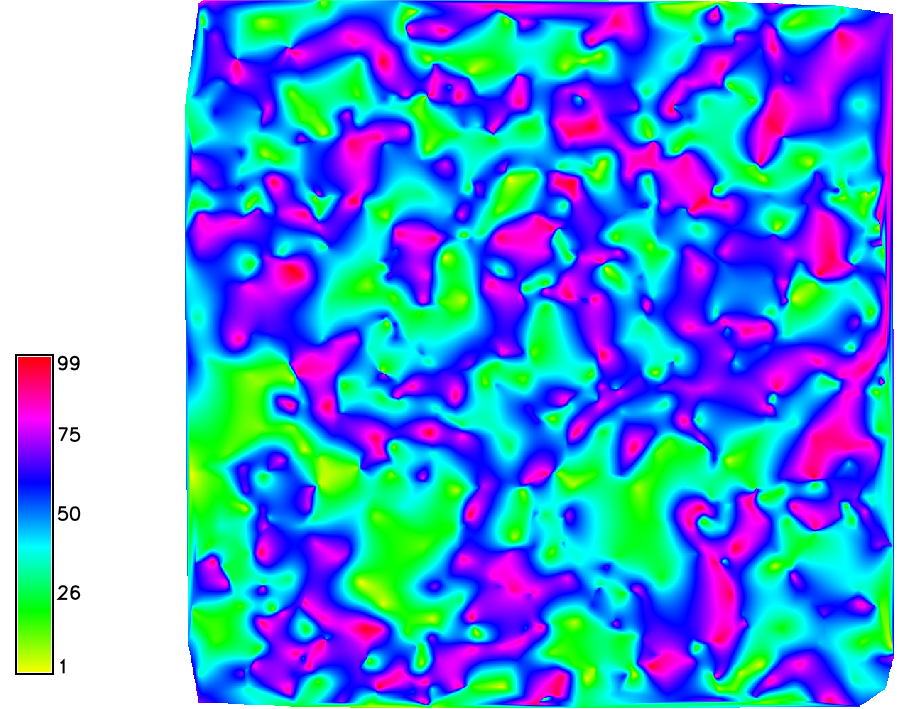
\includegraphics[width=0.48\textwidth]{img/body_1000.png}}{\caption{ArcGIS: Výstupní rastr pro 1000 bodů}}{\label{fig:b1000_Arc}}
\ffigbox{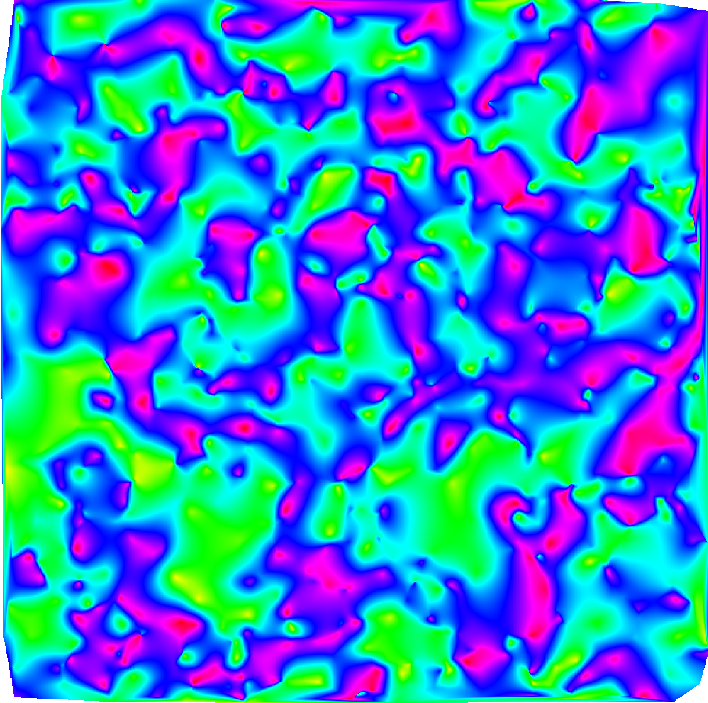
\includegraphics[width=0.48\textwidth]{img/body_1000_grass.png}}{\caption{GRASS GIS: Výstupní rastr pro 1000 bodů}}{\label{fig:b1000_grass}}
\end{floatrow}
\end{figure}

\begin{figure}[h!]
\centering
\begin{floatrow}
\ffigbox{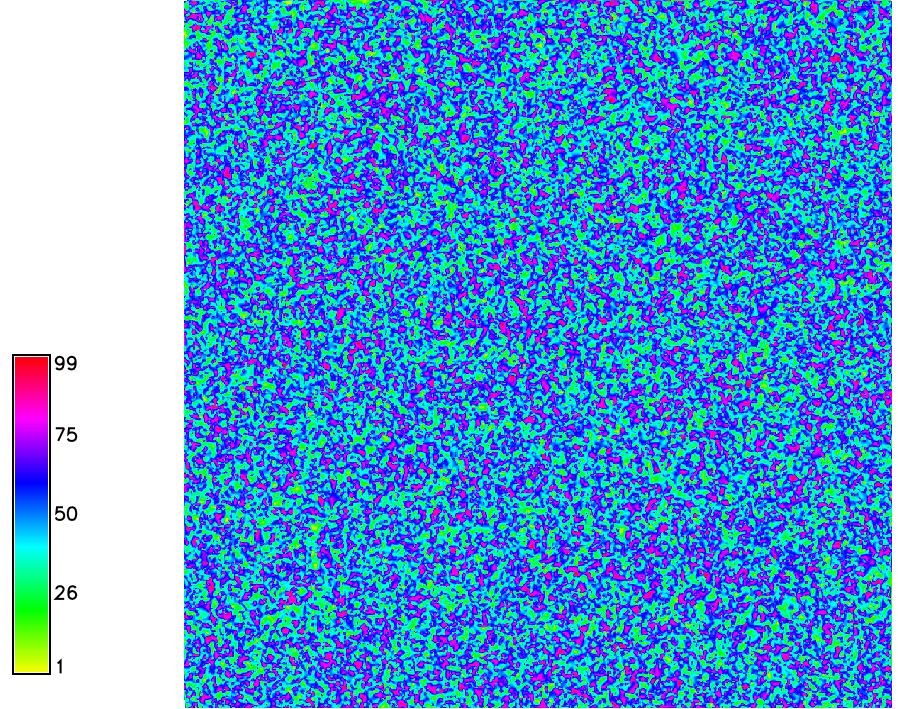
\includegraphics[width=0.48\textwidth]{img/body_100000.png}}{\caption{ArcGIS: Výstupní rastr pro 100000 bodů}}{\label{fig:b100000_Arc}}
\ffigbox{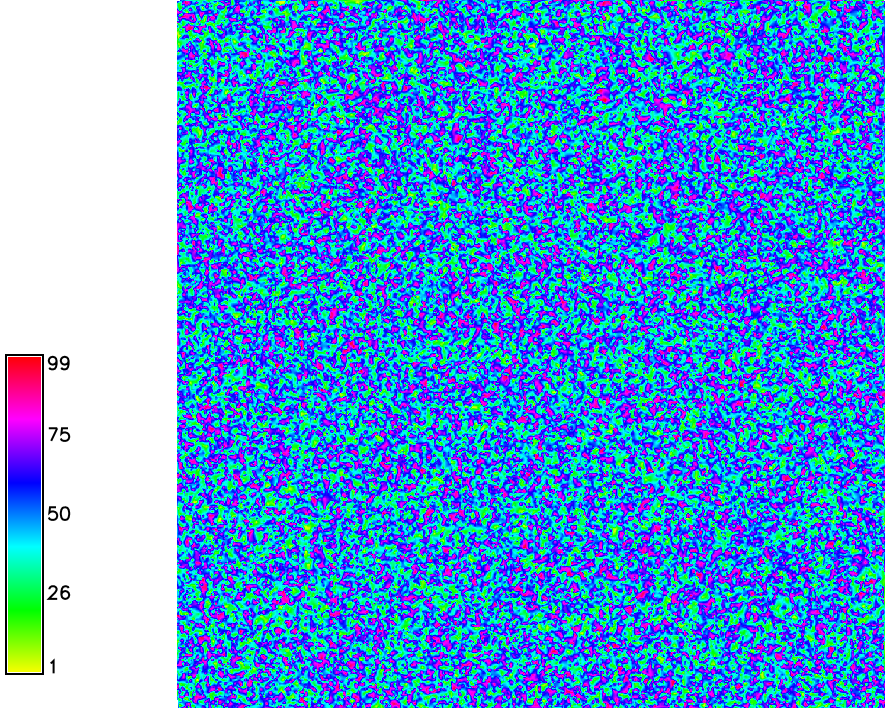
\includegraphics[width=0.48\textwidth]{img/body_100000_grass.png}}{\caption{GRASS GIS: Výstupní rastr pro 100000 bodů}}{\label{fig:b100000_grass}}
\end{floatrow}
\end{figure}

%%% ML: pozor, tady mas stale GRASS

\newpage
\begin{figure}[h!]
\centering
\begin{floatrow}
\ffigbox{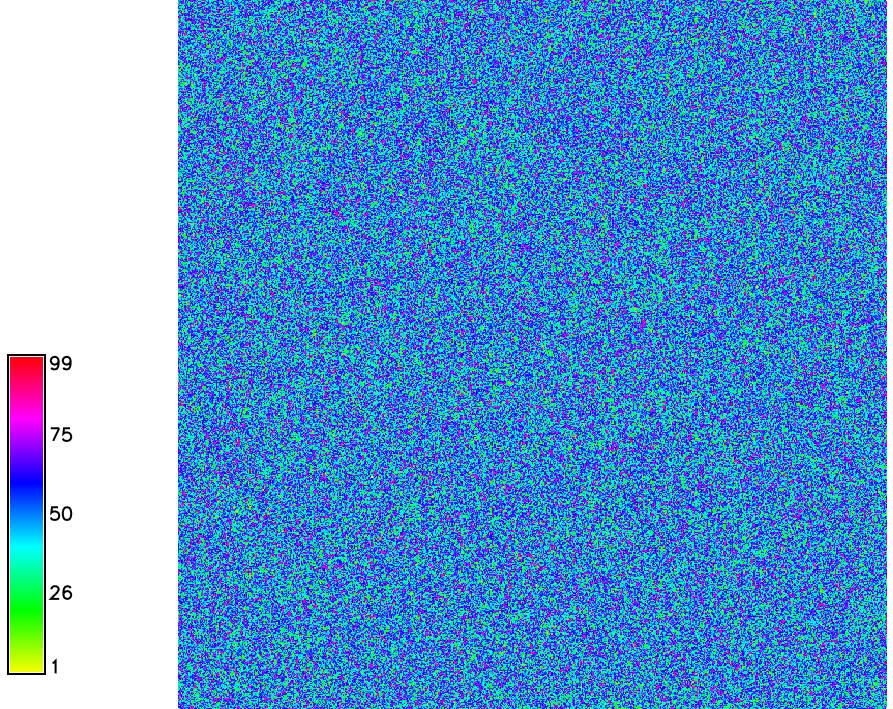
\includegraphics[width=0.48\textwidth]{img/body_mil_grass.png}}{\caption{ArcGIS: Výstupní rastr pro 1000000 bodů}}{\label{fig:b_mil_Arc}}
\ffigbox{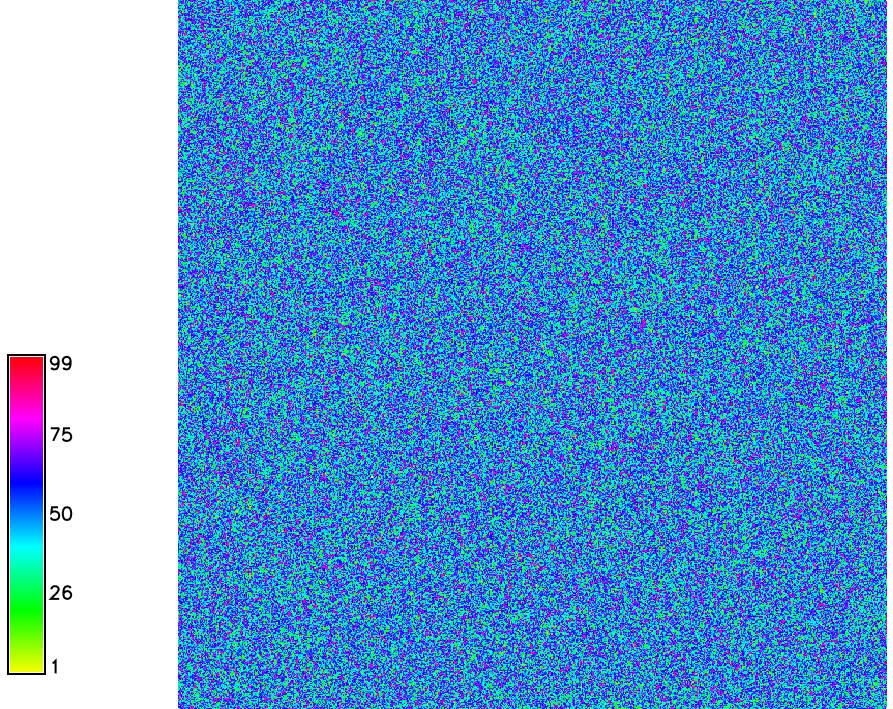
\includegraphics[width=0.48\textwidth]{img/body_mil_grass.png}}{\caption{GRASS GIS: Výstupní rastr pro 1000000 bodů}}{\label{fig:b_mil_grass}}
\end{floatrow}
\end{figure}

\newpage
\section{Delaunay struktura}
\label{app:delaunay_struct}
\lstinputlisting[language=C]{../src/nnbathy/delaunay_struct.h}

\newpage
\section{Winged-edge struktura}
\label{app:edge_struct}
\lstinputlisting[language=C]{../src/nnbathy/edge_struct.h}

%%% ML: je otazka zda kompletni zdrove kody uvadet do prilohy, pokud
%%% ano, tak pouze casti, na ktere se bude odkazovat v textu
\newpage
\section{Zdrojové kódy}
\subsection{nnbathy.py}
\label{app:nnbathy}
\lstinputlisting[language=Python]{../src/nnbathy/nn_red.py}

\bigskip
\subsection{v.surf.nnbathy.py}
\label{app:v.surf}
\lstinputlisting[language=Python]{../src/nnbathy/v_red.py}

\newpage
\subsection{r.surf.nnbathy.py}
\label{app:r.surf}
\lstinputlisting[language=Python]{../src/nnbathy/r_red.py}

%%% ML: chyby priloha Obsah CD/DVD
%%% AL: doplneno
\newpage
\section{Seznam tabulek}
\listoftables

\section{Seznam obrázků}
\listoffigures

\section{Obsah CD}

\setlength{\unitlength}{.5mm}
\begin{picture}(250, 220)
  \put(  0, 212){\textbf{.}}
  \put(  1, 200){\line(0, 1){5}}
  \put(  1, 200){\line(1, 0){10} {\textbf{ text}}}
  \put( 16, 190){\line(0, 1){8}}
  \put( 16, 190){\line(1, 0){10} {\textbf{ LaTeX}}}
  \put(150, 190){ zdrojové soubory textu}
  \put( 16, 180){\line(0, 1){10}}
  \put( 16, 180){\line(1, 0){10} { adam-laza-bp-2015.pdf}}
  \put(150, 180){ tento text}
  \put( 16, 170){\line(0, 1){10}}
  \put( 16, 170){\line(1, 0){10} { adam-laza-bp-2015.xls}}
  \put(150, 170){ anotace práce}
  \put( 16, 160){\line(0, 1){10}}
  \put( 16, 160){\line(1, 0){10} { zadani.pdf}}
  \put(150, 160){ naskenované oficiální zadání této práce}
  \put(  1, 150){\line(0, 1){60}}
  \put(  1, 150){\line(1, 0){10} {\textbf{ src}}}
  \put( 16, 140){\line(0, 1){8}}
  \put( 16, 140){\line(1, 0){10} {\textbf{ nnbathy}}}
  \put(150, 140){ zdrojové kódy nnbathy}
  \put( 16, 130){\line(0, 1){10}}
  \put( 16, 130){\line(1, 0){10} {\textbf{ cgal}}}
  \put(150, 130){ zdrojové kódy cgal}
  \put(  1, 120){\line(0, 1){50}}
  \put(  1, 120){\line(1, 0){10} {\textbf{ testing}}}
  \put( 16, 110){\line(0, 1){8}}
  \put( 16, 110){\line(1, 0){10} {\textbf{ src}}}
  \put(150, 110){ zdrojové soubory testovací aplikace}
  \put( 16, 100){\line(0, 1){10}}
  \put( 16, 100){\line(1, 0){10} {\textbf{ sample\_data}}}
  \put(150, 100){ testovací data}
\end{picture}
\end{document}
